%%%%%%%%%%%%%%%%%%%%%%%%%%%%%%%%%%%%%%%%%%%%%%%%%%%%%%%%%%%%%%%%%%%%%%%%
% Uni Duesseldorf
% Lehrstuhl fuer Datenbanken und Informationssysteme
% Vorlage fuer Bachelor-/Masterarbeiten
% Optimiert fuer den Original-Latex-Kompiler LATEX.EXE (LaTeX=>PS=>PDF)
%%%%%%%%%%%%%%%%%%%%%%%%%%%%%%%%%%%%%%%%%%%%%%%%%%%%%%%%%%%%%%%%%%%%%%%%
% Ueberarbeitung für pdflatex (LaTeX=>PDF)
%%%%%%%%%%%%%%%%%%%%%%%%%%%%%%%%%%%%%%%%%%%%%%%%%%%%%%%%%%%%%%%%%%%%%%%%
% Vorlage Changelog:
% 10.09.2015 (Matthias Liebeck): Nummerierung des Inhaltsverzeichnis nun römisch, Beispiel für einen Anhang eingebaut, \raggedbottom hinter sections eingefügt
% 11.07.2018 (Matthias Liebeck): Ersetzung des Bibliographiestils, Einsatz von Biber
% 04.09.2018 (Matthias Liebeck):
%   * Bibtex: unnötige Bibtexfelder beim Rendern ausblenden (thx @ Markus Brenneis)
%   * ngerman: "et al." im BibTeX für drei oder mehr Autoren
%   * Neuer Befehl \sectionforcestartright: Sections immer rechts beginnen (thx @ Philipp Grawe)
%   * ngerman: Deutsche Anführungszeichen im Literaturverzeichnis (thx @ Markus Brenneis)
%   * ngerman: Deutsche Anführungszeichen im Literaturverzeichnis (thx @ Markus Brenneis)
% 16.10.2018 (Matthias Liebeck): Zwei fixes an \sectionforcestartright (thx @ Markus Brenneis)
%%%%%%%%%%%%%%%%%%%%%%%%%%%%%%%%%%%%%%%%%%%%%%%%%%%%%%%%%%%%%%%%%%%%%%%%
%%%% BEGINN EINSTELLUNG FUER DIE ARBEIT. UNBEDINGT ERFORDERLICH! %%%%%%%
%%%%%%%%%%%%%%%%%%%%%%%%%%%%%%%%%%%%%%%%%%%%%%%%%%%%%%%%%%%%%%%%%%%%%%%%
% Geben Sie Ihren Namen hier an:

\newcommand{\bearbeiter}{Julian Winter}

% Geben Sie hier den Titel Ihrer Arbeit an:
\newcommand{\titel}{Classification of Electrocardiograms using Contrastive Predictive Coding}

% Geben Sie das Datum des Beginns und Ende der Bachelorarbeit ein:
\newcommand{\beginndatum}{18.~August~2021}
\newcommand{\abgabedatum}{18.~Februar~2022}

% Geben Sie die Namen des Erst- und Zweitgutachters an:
\newcommand{\erstgutachter}{Prof. Dr. Stefan Harmeling}
\newcommand{\zweitgutachter}{Prof. Dr. Michael Leuschel}

% Falls Sie die Arbeit zweiseitig ausdrucken wollen,
% benutzen Sie die folgende Zeile mit
% \AN fuer zweiseitigen Druck
% \AUS fuer einseitigen Druck
\newcommand{\zweiseitig}{\AN}
% true fuer biber, false fuer klassischen Zitierstil
%\newcommand{\biber}{false}
\newcommand{\biber}{true}

% Falls Sections immer rechts beginnen sollen. Gerade für Masterarbeiten
% interessant. Bei kurzen Bachelorarbeiten eher weniger zu verwenden.
%\newcommand{\sectionforcestartright}{false}
\newcommand{\sectionforcestartright}{true}

% Falls die Arbeit in englischer Sprache verfasst
% werden soll, dann benutzen Sie die folgende Zeile mit
% englisch fuer englische Sprache
% deutsch fuer deutsche Sprache
\newcommand{\sprache}{englisch}

% Hier wird eingestellt, ob es sich bei der Arbeit um eine Bachelor-
% oder Masterarbeit handelt (unpassendes auskommentieren!):
\newcommand{\arbeit}{Masterarbeit}
%~ \newcommand{\arbeit}{Masterarbeit}


%%%%%%%%%%%%%%%%%%%%%%%%%%%%%%%%%%%%%%%%%%%%%%%%%%%%%%%%%%%%%%%%%%%%%%%%
%%%% ENDE EINSTELLUNGEN %%%%%%%%%%%%%%%%%%%%%%%%%%%%%%%%%%%%%%%%%%%%%%%%
%%%%%%%%%%%%%%%%%%%%%%%%%%%%%%%%%%%%%%%%%%%%%%%%%%%%%%%%%%%%%%%%%%%%%%%%

% Die folgende Zeile NICHT EDITIEREN oder loeschen


%%%%%%%%%%%%%%%%%%%%%%%%%%%%%%%%%%%%%%%%%%%%%%%%%%%%%%%%%%%
% Obere Titelmakros. Editieren Sie diese Datei nur, wenn
% Sie sich ABSOLUT sicher sind, was Sie da tun!!!
% (Z.B. zum Abaendern der BA-Vorlage in eine MA-Vorlage)
% Uni Duesseldorf
% Lehrstuhl fuer Datenbanken und Informationssysteme
% Version 2.2 - 2.3.2010
%%%%%%%%%%%%%%%%%%%%%%%%%%%%%%%%%%%%%%%%%%%%%%%%%%%%%%%%%%%
\newcommand{\AN}{twoside}
\newcommand{\AUS}{}


%\newcommand{\englisch}{}
%\newcommand{\deutsch}{\usepackage[german]{babel}}

%% Die folgenden auskommentierten Optionen dienen der automatischen
%% Erkennung des Latex-Kompilers und dem Setzen der davon abhängigen
%% Einstellungen. Bei Problem z.B. mit dem Einbinden von verschiedenen
%% Grafiktypen bei Verwendung von PdfLatex oder Latex, einfach die
%% verschiedenen \usepackage(s) ausprobieren. (Mit diesen Einstellungen
%% funktionierte diese Vorlage bei der Verwenundg von latex.exe als
%% Kompiler bei den meisten Studierenden.)

%\newif\ifpdf \ifx\pdfoutput\undefined
%\pdffalse % we are not running pdflatex
%\else
%\pdfoutput=1 % we are running pdflatex
%\pdfcompresslevel=9 % compression level for text and image;
%\pdftrue \fi

\documentclass[11pt,a4paper, \zweiseitig]{article}
\usepackage{ifthen}


\usepackage{amsmath,amssymb}
%\usepackage[iso]{umlaute}
\usepackage[utf8]{inputenc}
\usepackage{palatino} % palatino Schriftart
%\usepackage{makeidx} % um ein Index zu erstellen
\usepackage[nottoc]{tocbibind}
\usepackage[T1]{fontenc} %fuer richtige Trennung bei Umlauten
\usepackage{fancybox} % fuer die Rahmen
\usepackage{shortvrb}
\usepackage{url}
\usepackage[table]{xcolor}
\usepackage[font=footnotesize, labelfont=bf]{subcaption}
\usepackage{graphicx}%[draft]
\usepackage{courier}
\usepackage{forest}
\usepackage{pdfpages}
%\usepackage{standalone}
%\usepackage{hyperref}
\usepackage[]{algorithm2e}
\newcommand\mycommfont[1]{\footnotesize\ttfamily\color{codegreen}{#1}}
%\SetCommentSty{mycommfont}
\usepackage{booktabs}
\usepackage{csquotes}
\usepackage{longtable}
\usepackage{tabularx}
\usepackage{adjustbox}
\usepackage{soul}
\sethlcolor{lightgray}
\usepackage{float}
\usepackage{enumitem}
\usepackage{multirow}
\usepackage[font=footnotesize, labelfont=bf]{caption}
\captionsetup{font=footnotesize}
\captionsetup[figure]{font=footnotesize}
\captionsetup[table]{font=footnotesize}

\usepackage{tcolorbox}
\usepackage{listings}
\usepackage{xcolor}
%TODO:printer
%\pdfimageresolution=300 
%\usepackage{titletoc}
%\usepackage[loadonly]{titlesec}
%TODO: printer
\usepackage[colorlinks,citecolor=black,linkcolor=black]{hyperref}
%\usepackage[colorlinks,citecolor=blue,linkcolor=red]{hyperref} %anklickbares Inhaltsverzeichnis
\DeclareMathSymbol{*}{\mathbin}{symbols}{"01}
\DeclareMathOperator*{\mean}{mean}
\DeclareMathOperator*{\std}{std}

\def\chapterautorefname{Chapter}%
\def\sectionautorefname{Section}%
\def\subsectionautorefname{Subsection}%
\def\subsubsectionautorefname{Subsubsection}%
\def\paragraphautorefname{Paragraph}%
\def\tableautorefname{Table}%
\def\equationautorefname{Equation}%

\newlength\mystoreparindent
\newenvironment{myparindent}[1]{%
	\setlength{\mystoreparindent}{\the\parindent}
	\setlength{\parindent}{#1}
}{%
	\setlength{\parindent}{\mystoreparindent}
}

\definecolor{codegreen}{rgb}{0,0.6,0}
\definecolor{codegray}{rgb}{0.5,0.5,0.5}
\definecolor{codepurple}{rgb}{0.58,0,0.82}
\definecolor{backcolour}{rgb}{0.95,0.95,0.92}

\lstdefinestyle{mystyle}{
	backgroundcolor=\color{backcolour},   
	commentstyle=\color{codegreen},
	keywordstyle=\color{magenta},
	numberstyle=\tiny\color{codegray},
	stringstyle=\color{codepurple},
	basicstyle=\ttfamily\footnotesize,
	breakatwhitespace=false,         
	breaklines=true,                 
	captionpos=b,                    
	keepspaces=true,                 
	numbers=left,                    
	numbersep=5pt,                  
	showspaces=false,                
	showstringspaces=false,
	showtabs=false,                  
	tabsize=3
}

\lstset{
	style=mystyle,
	literate=
	{á}{{\'a}}1 {é}{{\'e}}1 {í}{{\'i}}1 {ó}{{\'o}}1 {ú}{{\'u}}1
	{Á}{{\'A}}1 {É}{{\'E}}1 {Í}{{\'I}}1 {Ó}{{\'O}}1 {Ú}{{\'U}}1
	{à}{{\`a}}1 {è}{{\`e}}1 {ì}{{\`i}}1 {ò}{{\`o}}1 {ù}{{\`u}}1
	{À}{{\`A}}1 {È}{{\'E}}1 {Ì}{{\`I}}1 {Ò}{{\`O}}1 {Ù}{{\`U}}1
	{ä}{{\"a}}1 {ë}{{\"e}}1 {ï}{{\"i}}1 {ö}{{\"o}}1 {ü}{{\"u}}1
	{Ä}{{\"A}}1 {Ë}{{\"E}}1 {Ï}{{\"I}}1 {Ö}{{\"O}}1 {Ü}{{\"U}}1
	{â}{{\^a}}1 {ê}{{\^e}}1 {î}{{\^i}}1 {ô}{{\^o}}1 {û}{{\^u}}1
	{Â}{{\^A}}1 {Ê}{{\^E}}1 {Î}{{\^I}}1 {Ô}{{\^O}}1 {Û}{{\^U}}1
	{ã}{{\~a}}1 {ẽ}{{\~e}}1 {ĩ}{{\~i}}1 {õ}{{\~o}}1 {ũ}{{\~u}}1
	{Ã}{{\~A}}1 {Ẽ}{{\~E}}1 {Ĩ}{{\~I}}1 {Õ}{{\~O}}1 {Ũ}{{\~U}}1
	{œ}{{\oe}}1 {Œ}{{\OE}}1 {æ}{{\ae}}1 {Æ}{{\AE}}1 {ß}{{\ss}}1
	{ű}{{\H{u}}}1 {Ű}{{\H{U}}}1 {ő}{{\H{o}}}1 {Ő}{{\H{O}}}1
	{ç}{{\c c}}1 {Ç}{{\c C}}1 {ø}{{\o}}1 {å}{{\r a}}1 {Å}{{\r A}}1
}

\ifthenelse{\boolean{\biber}}{
  % only needed for biber
  \usepackage[style=numeric,natbib=true,backend=biber,mincitenames=1,maxcitenames=2,maxbibnames=99,uniquelist=true, sorting=none]{biblatex}%style=authoryear,dashed=false

  % https://tex.stackexchange.com/a/334703/8850
  \AtEveryBibitem{%
    \clearfield{issn}
    \clearfield{isbn}
    \clearfield{doi}
    \clearfield{location}
    \clearlist{location}
    \clearlist{address}

    \ifentrytype{online}{}{% Remove url except for @online
      \clearfield{url}
    }
  }
}
{}%no else

% Falls es bei \citet ein Komma zwischen Name und Jahr gibt:
% https://tex.stackexchange.com/questions/312539/unwanted-comma-between-author-and-year-using-citet-command
% (thx @ Markus Brenneis)
%\DeclareDelimFormat[cbx@textcite]{nameyeardelim}{\addspace}



\ifthenelse{\equal{\sprache}{deutsch}}{
  \usepackage[ngerman]{babel}
  % Bibtex u.a -> et al.
  \ifthenelse{\boolean{\biber}}{
    \DefineBibliographyStrings{ngerman}{
      andothers = {{et\,al\adddot}},
    }
    \newcommand{\references}{Literatur}
  }
  {} % do nothing when not using biber
  \usepackage[autostyle, german=quotes]{csquotes} % Deutsche Anführungszeichen im Literaturverzeichnis (thx @ Markus Brenneis)

}{ \newcommand{\references}{References}
\usepackage[english]{babel}
}

\usepackage{a4wide} % ganze A4 Weite verwenden



%\ifpdf
%\usepackage[pdftex,xdvi]{graphicx}
%\usepackage{thumbpdf} %thumbs fuer Pdf
%\usepackage[pdfstartview=FitV]{hyperref} %anklickbares Inhaltsverzeichnis
%\else
%\usepackage[dvips,xdvi]{graphicx}
\usepackage{amsmath}

\newcommand{\code}[1]{\texttt{#1}}

%\fi

\newcommand{\redt}[1] {
  \textcolor{red}{#1}}

\DeclareRobustCommand{\bbone}{\text{\usefont{U}{bbold}{m}{n}1}}
\DeclareMathOperator{\EX}{\mathbb{E}} %expected value

\newcommand{\oranget}[1] {
  \textcolor{orange}{#1}}

\newcommand{\purplet}[1] {
  \textcolor{purple}{#1}}

%%%%%%%%%%%%%%%%%%%%%%% Massangaben fuer die Arbeit %%%%%%%%%%%%%%%
\setlength{\textwidth}{15cm}

\setlength{\oddsidemargin}{35mm}
\setlength{\evensidemargin}{25mm}

\addtolength{\oddsidemargin}{-1in}
\addtolength{\evensidemargin}{-1in}

\ifthenelse{\boolean{\biber}}{\addbibresource{references.bib}}{}

%\makeindex
\begin{document}
%\startcontents
\setcounter{secnumdepth}{5} %Nummerieren bis in die 4. Ebene
\setcounter{tocdepth}{5} %Inhaltsverzeichnis bis zur 4. Ebene

\pagestyle{headings}

\sloppy % LaTeX ist dann nicht so streng mit der Silbentrennung
%~ \MakeShortVerb{\§}

\parindent0mm
\parskip0.5em


{
\textwidth170mm
\oddsidemargin30mm
\evensidemargin30mm
\addtolength{\oddsidemargin}{-1in}
\addtolength{\evensidemargin}{-1in}

\parskip0pt plus2pt

% Die Raender muessen eventuell fuer jeden Drucker individuell eingestellt
% werden. Dazu sind die Werte fuer die Abstaende `\oben' und `\links' zu
% aendern, die von mir auf jeweils 0mm eingestellt wurden.

%\newlength{\links} \setlength{\links}{10mm}  % hier abzuaendern
%\addtolength{\oddsidemargin}{\links}
%\addtolength{\evensidemargin}{\links}

\begin{titlepage}
\vspace*{-1.5cm}
\raisebox{17mm}{
    \begin{minipage}[t]{70mm}
        \begin{center}
            %\selectlanguage{german}
            {\Large INSTITUT FÜR INFORMATIK\\}
            {\normalsize
                Machine Learning\\
            }
            \vspace{3mm}
            {\small Universitätsstr. 1 \hspace{5ex} D--40225 Düsseldorf\\}
        \end{center}
    \end{minipage}
}
\hfill
\raisebox{7mm}{
    
\includegraphics[width=130pt]{bilder/HHU_Logo}}
\vspace{14em}

% Titel
\begin{center}
    \baselineskip=55pt
    \textbf{\huge \titel}
    \baselineskip=0 pt
\end{center}

%\vspace{7em}

\vfill

% Autor
\begin{center}
    \textbf{\Large
        \bearbeiter
    }
\end{center}

\vspace{35mm}

% Prüfungsordnungs-Angaben
\begin{center}
%\selectlanguage{german}

%%%%%%%%%%%%%%%%%%%%%%%%%%%%%%%%%%%%%%%%%%%%%%%%%%%%%%%%%%%%%%%%%%%%%%%%%
% Ja, richtig, hier kann die BA-Vorlage zur MA-Vorlage gemacht werden...
% (nicht mehr nötig!)
%%%%%%%%%%%%%%%%%%%%%%%%%%%%%%%%%%%%%%%%%%%%%%%%%%%%%%%%%%%%%%%%%%%%%%%%%
{\Large \arbeit}

\vspace{2em}
\ifthenelse{\equal{\sprache}{deutsch}}{
    \begin{tabular}[t]{ll}
    Beginn der Arbeit:& \beginndatum \\
    Abgabe der Arbeit:& \abgabedatum \\
    Gutachter:         & \erstgutachter \\
    & \zweitgutachter \\
}{
    \begin{tabular}[t]{ll}
    Date of issue:& \beginndatum \\
    Date of submission:& \abgabedatum \\
    Reviewers:         & \erstgutachter \\
    & \zweitgutachter \\
}
\end{tabular}
\end{center}

\end{titlepage}

}

%%%%%%%%%%%%%%%%%%%%%%%%%%%%%%%%%%%%%%%%%%%%%%%%%%%%%%%%%%%%%%%%%%%%%
\clearpage
\begin{titlepage}
    ~                % eine leere Seite hinter dem Deckblatt
\end{titlepage}
%%%%%%%%%%%%%%%%%%%%%%%%%%%%%%%%%%%%%%%%%%%%%%%%%%%%%%%%%%%%%%%%%%%%%
\clearpage
\begin{titlepage}
    \vspace*{\fill}

    \section*{Erklärung}

    %%%%%%%%%%%%%%%%%%%%%%%%%%%%%%%%%%%%%%%%%%%%%%%%%%%%%%%%%%%
    % Und hier ebenfalls ggf. BA durch MA ersetzen...
    % (Auch nicht mehr nötig!)
    %%%%%%%%%%%%%%%%%%%%%%%%%%%%%%%%%%%%%%%%%%%%%%%%%%%%%%%%%%%

    Hiermit versichere ich, dass ich diese \arbeit{}
    selbstständig verfasst habe. Ich habe dazu keine anderen als die
    angegebenen Quellen und Hilfsmittel verwendet.

    \vspace{25 mm}

    \begin{tabular}{lc}
        Düsseldorf, den \abgabedatum \hspace*{2cm} & \underline{\hspace{6cm}} \\
                                                   & \bearbeiter
    \end{tabular}

    \vspace*{\fill}
\end{titlepage}

%%%%%%%%%%%%%%%%%%%%%%%%%%%%%%%%%%%%%%%%%%%%%%%%%%%%%%%%%%%%%%%%%%%%%
% Leerseite bei zweiseitigem Druck
%%%%%%%%%%%%%%%%%%%%%%%%%%%%%%%%%%%%%%%%%%%%%%%%%%%%%%%%%%%%%%%%%%%%%

\ifthenelse{\equal{\zweiseitig}{twoside}}{\clearpage\begin{titlepage}
        ~\end{titlepage}}{}

%%%%%%%%%%%%%%%%%%%%%%%%%%%%%%%%%%%%%%%%%%%%%%%%%%%%%%%%%%%%%%%%%%%%%
\clearpage
\begin{titlepage}

    %%% Die folgende Zeile nicht ändern!
%\section{Abstract}
%%% Zusammenfassung:

\begin{abstract}
The following work deals with classifying multilabel electro-cardiographic data using a \enquote{self-supervised} learning method called Contrastive Predictive Coding (short CPC) \autocite{DBLP:journals/corr/abs-1807-03748}, that learns lower dimensional data representations without requiring class labels. These data representations can then be used in classification tasks. Learning from data without labels is potentially very beneficial in fields where correctly labeled data is scarce and only obtainable slowly by human experts.

The goal of this work is to re-implement CPC, apply and test several changes to the architecture and evaluate its capability of classifying ECG-data. We try to answer the following central questions to shine a light on CPC's strengths and weaknesses:

How does the CPC architecture compare against our baseline models in a fully supervised setting? How capable is CPC's pretraining? How good are the learned representations on their own? Under what circumstances is CPC especially efficient to use? Can the original architecture be improved? Does CPC learn visually verifiable useful latent representations?
%What does CPC excel in? Is CPC always applicable as a pretraining step? Is the general CPC architecture suited for fully supervised training? Are the features extracted by CPC pretraining data descriptive? Does CPC work on heavily augmented data?

We will answer these questions by conducting various experiments that aim to emulate real-life circumstances such as low label availability and limited training times. CPC is compared to fully supervised models, where we make use of architectures like the TCN \autocite{bai2018empirical} and a special time-series classification focused residual net \autocite{yu2016multiscale}, but also introduce a wide variety of own baseline models. 

For evaluation we look at predictions both quantitatively, through different metrics, and qualitatively, by either inspecting embeddings in lower dimensions of the learned representations or by visualizing the prediction probabilities in a wide variety of plots. Additionally we utilize the gradient of selected trained networks to show spots in the input data which possibly contain ECG-classes. 

Our contributions to the field are a more precise explanation of the original publication \autocite{DBLP:journals/corr/abs-1807-03748}, alterations to the one dimensional architecture suited for timeseries classification, namely non overlapping data windows, normalized latent representations, different encoder-, autoregressive context- and downstream-task networks. We also introduce a "no-context" architecture which predict latents without making use of the standard context recurrent network. In total we trained and tested over 1700\footnote{We count individually trained/tested networks, not necessarily different architectures} networks and will also release their model properties and average scores as table for all those interested. 

Last but not least our generated prediction plots and "point of interest"-visualization mainly based on grad-cam \autocite{DBLP:journals/corr/SelvarajuDVCPB16}, show the different models' strengths beyond classification scores and could also assist cardiologists in the future. 


%First we start by giving insights about electro-cardiographic data, \enquote{self-supervised} learning methods in general and Contrastive Predictive Coding from the original paper \autocite{DBLP:journals/corr/abs-1807-03748} in closer detail. There we try to supply the reader with further information and possible explanations.
%
%Secondly the ECG-data is being looked at in detail, by visualizing the different class label amounts for both the complete data and our training dataset. Moreover the correlation between classes in pairs is shown as well, to get a better understanding of the data and classification problem.
%
%Next we re-implement CPC and additionally introduce and apply our modifications to the architecture. Multiple baselines have been implemented for comparison, including but not limited to different multilayered convolutional networks, as well as simple recurrent neural networks or the more recent Temporal Convolutional Network \autocite{bai2018empirical}, which aims to provide an alternative to recurrent architectures in time-series prediction.
%
%The work continues by explaining the training settings for the models and how the ECG-data is pre-processed.
%
%We conduct experiments to test for various circumstances such as low label availability, amount of parameters, training difficulty/duration and more, to show possible strengths or weaknesses of the architectures.
%
%Afterwards we present our detailed results where performance metrics are calculated and compared for all tested models. 
%
%Furthermore we visualize the class prediction probabilities per sample as scatter plot or on average in errorbars, in order to provide a more meaningful model output representation apart from scores.
%
%As a bonus we try to highlight regions in the input data that are interesting to the model architecture by calculating the gradient w.r.t. to input. There we also compare different models in their capability of producing clear results (TODO: and ask a cardiologist about their opinion. ?)

\end{abstract}


    %%%%%%%%%%%%%%%%%%%%%%%%%%%%%%%%%%%%%%%%%%%%%%%%
    % Untere Titelmakros. Editieren Sie diese Datei nur, wenn Sie sich
    % ABSOLUT sicher sind, was Sie da tun!!!
    %%%%%%%%%%%%%%%%%%%%%%%%%%%%%%%%%%%%%%%%%%%%%%%
    \vspace*{\fill}
\end{titlepage}

%%%%%%%%%%%%%%%%%%%%%%%%%%%%%%%%%%%%%%%%%%%%%%%%%%%%%%%%%%%%%%%%%%%%%
% Leerseite bei zweiseitigem Druck
%%%%%%%%%%%%%%%%%%%%%%%%%%%%%%%%%%%%%%%%%%%%%%%%%%%%%%%%%%%%%%%%%%%%%
\ifthenelse{\equal{\zweiseitig}{twoside}}
{\clearpage\begin{titlepage}~\end{titlepage}}{}
%%%%%%%%%%%%%%%%%%%%%%%%%%%%%%%%%%%%%%%%%%%%%%%%%%%%%%%%%%%%%%%%%%%%%
\clearpage \setcounter{page}{1}
\pagenumbering{roman}
%\setcounter{tocdepth}{5}
\begingroup\hypersetup{linkcolor=black}\tableofcontents\endgroup
%\begingroup\hypersetup{linkcolor=black}\printcontents{ }{0}{}\endgroup
%\tableofcontents

%\enlargethispage{\baselineskip}
\clearpage
%%%%%%%%%%%%%%%%%%%%%%%%%%%%%%%%%%%%%%%%%%%%%%%%%%%%%%%%%%%%%%%%%%%%%
% Leere Seite, falls Inhaltsverzeichnis mit ungerader Seitenzahl und
% doppelseitiger Druck
%%%%%%%%%%%%%%%%%%%%%%%%%%%%%%%%%%%%%%%%%%%%%%%%%%%%%%%%%%%%%%%%%%%%%
\ifthenelse{ \( \equal{\zweiseitig}{twoside} \and \not \isodd{\value{page}} \)}
{\pagebreak \thispagestyle{empty} \cleardoublepage}{\clearpage}


% Kapitel soll bei doppelseitigem Druck immer auf der rechten (ungeraden) Seite anfangen (thx @ Philipp Grawe)
% https://tex.stackexchange.com/a/223387
\ifthenelse{\boolean{\sectionforcestartright}}
{\let\oldsection\section % Store \section in \oldsection
    \renewcommand{\section}{\cleardoublepage\oldsection}}
{}
\pagenumbering{arabic}
\setcounter{page}{3} %1

%%%%%%%%%%%%%%%%%%%%%%%%%%%%%%%%%%%%%%%%%%%%%%%%%%%%%%%%%%%%%%%%%%%%%%%%
%%%% BEGINN TEXTTEIL %%%%%%%%%%%%%%%%%%%%%%%%%%%%%%%%%%%%%%%%%%%%%%%%%%%
%%%%%%%%%%%%%%%%%%%%%%%%%%%%%%%%%%%%%%%%%%%%%%%%%%%%%%%%%%%%%%%%%%%%%%%%

%%%%%%%%%%%%%%%%%%%%%%%%%%%%%%%%%%%%%%%%%%%%%%%%%%%%%%%%%%%%%%%%%%%%%%%%
% Text entweder direkt hier hinein schreiben oder, im Sinne der
% besseren Uebersichtlich- und Bearbeitbarkeit mittels \input die
% einzelnen Textteile hier einbinden.
%%%%%%%%%%%%%%%%%%%%%%%%%%%%%%%%%%%%%%%%%%%%%%%%%%%%%%%%%%%%%%%%%%%%%%%%
%%%% Die folgende Zeile nicht ändern!
%\section{Abstract}
%%% Zusammenfassung:

\begin{abstract}
The following work deals with classifying multilabel electro-cardiographic data using a \enquote{self-supervised} learning method called Contrastive Predictive Coding (short CPC) \autocite{DBLP:journals/corr/abs-1807-03748}, that learns lower dimensional data representations without requiring class labels. These data representations can then be used in classification tasks. Learning from data without labels is potentially very beneficial in fields where correctly labeled data is scarce and only obtainable slowly by human experts.

The goal of this work is to re-implement CPC, apply and test several changes to the architecture and evaluate its capability of classifying ECG-data. We try to answer the following central questions to shine a light on CPC's strengths and weaknesses:

How does the CPC architecture compare against our baseline models in a fully supervised setting? How capable is CPC's pretraining? How good are the learned representations on their own? Under what circumstances is CPC especially efficient to use? Can the original architecture be improved? Does CPC learn visually verifiable useful latent representations?
%What does CPC excel in? Is CPC always applicable as a pretraining step? Is the general CPC architecture suited for fully supervised training? Are the features extracted by CPC pretraining data descriptive? Does CPC work on heavily augmented data?

We will answer these questions by conducting various experiments that aim to emulate real-life circumstances such as low label availability and limited training times. CPC is compared to fully supervised models, where we make use of architectures like the TCN \autocite{bai2018empirical} and a special time-series classification focused residual net \autocite{yu2016multiscale}, but also introduce a wide variety of own baseline models. 

For evaluation we look at predictions both quantitatively, through different metrics, and qualitatively, by either inspecting embeddings in lower dimensions of the learned representations or by visualizing the prediction probabilities in a wide variety of plots. Additionally we utilize the gradient of selected trained networks to show spots in the input data which possibly contain ECG-classes. 

Our contributions to the field are a more precise explanation of the original publication \autocite{DBLP:journals/corr/abs-1807-03748}, alterations to the one dimensional architecture suited for timeseries classification, namely non overlapping data windows, normalized latent representations, different encoder-, autoregressive context- and downstream-task networks. We also introduce a "no-context" architecture which predict latents without making use of the standard context recurrent network. In total we trained and tested over 1700\footnote{We count individually trained/tested networks, not necessarily different architectures} networks and will also release their model properties and average scores as table for all those interested. 

Last but not least our generated prediction plots and "point of interest"-visualization mainly based on grad-cam \autocite{DBLP:journals/corr/SelvarajuDVCPB16}, show the different models' strengths beyond classification scores and could also assist cardiologists in the future. 


%First we start by giving insights about electro-cardiographic data, \enquote{self-supervised} learning methods in general and Contrastive Predictive Coding from the original paper \autocite{DBLP:journals/corr/abs-1807-03748} in closer detail. There we try to supply the reader with further information and possible explanations.
%
%Secondly the ECG-data is being looked at in detail, by visualizing the different class label amounts for both the complete data and our training dataset. Moreover the correlation between classes in pairs is shown as well, to get a better understanding of the data and classification problem.
%
%Next we re-implement CPC and additionally introduce and apply our modifications to the architecture. Multiple baselines have been implemented for comparison, including but not limited to different multilayered convolutional networks, as well as simple recurrent neural networks or the more recent Temporal Convolutional Network \autocite{bai2018empirical}, which aims to provide an alternative to recurrent architectures in time-series prediction.
%
%The work continues by explaining the training settings for the models and how the ECG-data is pre-processed.
%
%We conduct experiments to test for various circumstances such as low label availability, amount of parameters, training difficulty/duration and more, to show possible strengths or weaknesses of the architectures.
%
%Afterwards we present our detailed results where performance metrics are calculated and compared for all tested models. 
%
%Furthermore we visualize the class prediction probabilities per sample as scatter plot or on average in errorbars, in order to provide a more meaningful model output representation apart from scores.
%
%As a bonus we try to highlight regions in the input data that are interesting to the model architecture by calculating the gradient w.r.t. to input. There we also compare different models in their capability of producing clear results (TODO: and ask a cardiologist about their opinion. ?)

\end{abstract}

\section{Introduction}\raggedbottom

\subsection{Electrocardiographic Data}
Electrocardiographic data is obtained by placing electrodes on different parts of the body, mainly around the heart, which measure the electrical changes in voltage over time, produced by the heart muscle \autocite{ElectrocardiographyWikipedia-2021-01-14}. Multiple electrodes are placed to get a better overview over the heart state, since other muscles will add noise under non ideal conditions. A high recording frequency of 257-10000hz and a recording length of 10 seconds up to 30 minutes\footnote{attributes of ECG data reported from \ref{itm:itemize-datas}} or even days (long time ECG used in hospitals) are desirable to not miss important information that could reveal an infarction and other muscular heart diseases.
 
We obtain sequential data that can be classified like other time-series, however since each individual electrode produces its own signal there is more than one data channel to analyze concurrently, which increases the difficulty to find a generalizing computer system. For example the conventional "12-lead ECG" uses 10 differently placed electrodes resulting in 12 different channels together with the two additional ones added by averaging \autocite{12LeadECGPlacementGuidewithIllustrations-2021-09-28}. Accounting for the high frequency and length this would sum up to $\mathbf{data points}=\mathbf{seconds}*\mathbf{frequency}*\mathbf{channels}=10\mathbf{s}*1000\mathbf{hz}*12=120000$ data points for short recordings or $120\mathbf{s}*1000\mathbf{hz}*12=1440000$ data points for longer recordings, per patient (assuming a frequency of 1000hz). The varying lengths and much information make correct prediction challenging. For comparison, the widely used ImageNet \autocite{ImageNet-2021-01-14} counts on average $469\times387$ pixels\autocite{stack-imagenet}, which is equal to $469*387*3=544509$ data points. Additionally the recordings can contain more than one \enquote{true} label which makes correct classification even more difficult. Like in many medical fields, one big hurdle in training a fully automated system is the inaccessible correctly labeled data. The biggest reason for the data scarcity is that only trained professionals/doctors are able to successfully diagnose patients, while also requiring long periods of time to do so.  

Nevertheless we found a few dataset sources that are openly available online:
\begin{itemize}
	\item[PTB] A dataset provided by the Physikalisch-Technische Bundesanstalt (PTB) containing 549 records with 9 diagnostic class labels. \autocite{ptb}
	\item[PTB-XL] A dataset provided by the Physikalisch-Technische Bundesanstalt (PTB) containining 21837 records with 52 diagnostic class labels (5 superclasses, split into 52 unique scp codes).\autocite{ptbxl}
	\item[Georgia] \enquote{Georgia} dataset which is hosted on \url{Kaggle.com} \autocite{Georgia12LeadECGChallengeDatabaseKaggle-2021-03-15}
	\item[China] A dataset provided during a chinese classification challenge and made openly available.
	\item[Nature] A 12-lead electrocardiogram database for arrhythmia research covering more than 10,000 patients. \autocite{Zheng2020}
	\label{itm:itemize-datas}
\end{itemize}
Most of the above datasets and more are also used in a recent ECG classification challenge from 2020 \autocite{PerezAlday2021} hosted by physionet.org \autocite{physionet}. Since the original datasets have incompatible labels (e.g. the same classes are mapped to different terms) we use the available challenge data because the labels across all datasets were already mapped to unique SNOMED CT codes \autocite{SNOMEDCTClasses}. The \enquote{Nature} data labels, which are not part of the challenge data, had to be dropped since they were incompatible to the other datasets, thus this data will be only used in pretraining for models that require it.

The data has 12 channels and one or more \enquote{true} labels per sample. However there is no hint on to where the label is found in the sequential data. See \autoref{fig:ECGBasic} for an example ECG recording.
\begin{figure}[H]
	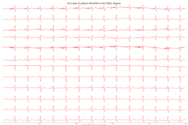
\includegraphics[width=\textwidth]{bilder/ecg-example0.png}
	\caption{A single patients ECG with 500hz recording frequency. The classes \textit{EKG: T wave abnormal} and \textit{sinus rhythm} can both be found somewhere in the data.}
	\label{fig:ECGBasic}
\end{figure}
To better understand the data we count class occurrences over all datasets, with their respective SNOMED Code and the index number used in our implementation \autoref{table:ClassCounts}. Readily identifiable is that not every class is present in all datasets and that some classes are very rare in comparison to others. Additionally some classes are closely related or even superclasses of others but are not consistently stated as true even though the subclass is true (see Bundle Branch Block vs. left/right Bundle Branch Block or Ventricular Hypertrophy vs. left/right Ventricular Hypertrophy). Since some class distinctions might be intentional, we did not apply any changes to the labels, but want to point out the possible classification difficulty increase due to the label inconsistencies. 

\begin{figure}[H]
	\caption{All SNOMED Codes with their respective name and count in the datasets.}
	\resizebox{!}{0.8\textwidth}{
		\begin{tabular}{lllrrrr}
{} & {} & {} & {ptbxl} & {georgia} & {cpsc} & {cpsc2} \\
{Index} & {Class Snomed Code} & {Class Term} & {} & {} & {} & {} \\
0 & 10370003 & Rhythm from artificial pacing (298) & {\cellcolor[HTML]{2E8B57}} \color[HTML]{F1F1F1} 295 & {\cellcolor[HTML]{EBF3ED}} \color[HTML]{000000} 0 & {\cellcolor[HTML]{EBF3ED}} \color[HTML]{000000} 0 & {\cellcolor[HTML]{E9F2EC}} \color[HTML]{000000} 3 \\
1 & 11157007 & Ventricular bigeminy (89) & {\cellcolor[HTML]{2E8B57}} \color[HTML]{F1F1F1} 82 & {\cellcolor[HTML]{E7F0EA}} \color[HTML]{000000} 2 & {\cellcolor[HTML]{EBF3ED}} \color[HTML]{000000} 0 & {\cellcolor[HTML]{E0ECE4}} \color[HTML]{000000} 5 \\
2 & 111975006 & Prolonged QT interval (1493) & {\cellcolor[HTML]{DBEAE0}} \color[HTML]{000000} 118 & {\cellcolor[HTML]{2E8B57}} \color[HTML]{F1F1F1} 1372 & {\cellcolor[HTML]{EBF3ED}} \color[HTML]{000000} 0 & {\cellcolor[HTML]{EBF3ED}} \color[HTML]{000000} 3 \\
3 & 164861001 & EKG myocardial ischemia (2556) & {\cellcolor[HTML]{2E8B57}} \color[HTML]{F1F1F1} 2175 & {\cellcolor[HTML]{EBF3ED}} \color[HTML]{000000} 0 & {\cellcolor[HTML]{EBF3ED}} \color[HTML]{000000} 0 & {\cellcolor[HTML]{CAE1D3}} \color[HTML]{000000} 381 \\
4 & 164865005 & EKG: myocardial infarction (5640) & {\cellcolor[HTML]{2E8B57}} \color[HTML]{F1F1F1} 5261 & {\cellcolor[HTML]{EBF3ED}} \color[HTML]{000000} 7 & {\cellcolor[HTML]{EBF3ED}} \color[HTML]{000000} 0 & {\cellcolor[HTML]{DEEBE3}} \color[HTML]{000000} 372 \\
5 & 164867002 & EKG: old myocardial infarction (1160) & {\cellcolor[HTML]{EBF3ED}} \color[HTML]{000000} 0 & {\cellcolor[HTML]{EBF3ED}} \color[HTML]{000000} 0 & {\cellcolor[HTML]{EBF3ED}} \color[HTML]{000000} 0 & {\cellcolor[HTML]{2E8B57}} \color[HTML]{F1F1F1} 1160 \\
6 & 164873001 & EKG:left ventricle hypertrophy (3735) & {\cellcolor[HTML]{2E8B57}} \color[HTML]{F1F1F1} 2359 & {\cellcolor[HTML]{88BD9F}} \color[HTML]{000000} 1226 & {\cellcolor[HTML]{EBF3ED}} \color[HTML]{000000} 0 & {\cellcolor[HTML]{DFECE4}} \color[HTML]{000000} 150 \\
7 & 164884008 & ECG: ventricular ectopics (1894) & {\cellcolor[HTML]{2E8B57}} \color[HTML]{F1F1F1} 1154 & {\cellcolor[HTML]{E4EFE8}} \color[HTML]{000000} 41 & {\cellcolor[HTML]{78B492}} \color[HTML]{F1F1F1} 699 & {\cellcolor[HTML]{EBF3ED}} \color[HTML]{000000} 0 \\
8 & 164889003 & ECG: atrial fibrillation (3441) & {\cellcolor[HTML]{2E8B57}} \color[HTML]{F1F1F1} 1514 & {\cellcolor[HTML]{B2D3C0}} \color[HTML]{000000} 561 & {\cellcolor[HTML]{57A177}} \color[HTML]{F1F1F1} 1219 & {\cellcolor[HTML]{EBF3ED}} \color[HTML]{000000} 147 \\
9 & 164890007 & EKG: atrial flutter (303) & {\cellcolor[HTML]{A0CAB2}} \color[HTML]{000000} 73 & {\cellcolor[HTML]{2E8B57}} \color[HTML]{F1F1F1} 185 & {\cellcolor[HTML]{EBF3ED}} \color[HTML]{000000} 0 & {\cellcolor[HTML]{BDD9C9}} \color[HTML]{000000} 45 \\
10 & 164909002 & EKG: left bundle branch block (1038) & {\cellcolor[HTML]{2E8B57}} \color[HTML]{F1F1F1} 536 & {\cellcolor[HTML]{A2CBB3}} \color[HTML]{000000} 229 & {\cellcolor[HTML]{A0CAB2}} \color[HTML]{000000} 235 & {\cellcolor[HTML]{EBF3ED}} \color[HTML]{000000} 38 \\
11 & 164917005 & EKG: Q wave abnormal (1010) & {\cellcolor[HTML]{2E8B57}} \color[HTML]{F1F1F1} 548 & {\cellcolor[HTML]{4C9B6F}} \color[HTML]{F1F1F1} 461 & {\cellcolor[HTML]{EBF3ED}} \color[HTML]{000000} 0 & {\cellcolor[HTML]{EBF3ED}} \color[HTML]{000000} 1 \\
12 & 164930006 & ECG: ST interval abnormal (1453) & {\cellcolor[HTML]{EBF3ED}} \color[HTML]{000000} 0 & {\cellcolor[HTML]{2E8B57}} \color[HTML]{F1F1F1} 979 & {\cellcolor[HTML]{EBF3ED}} \color[HTML]{000000} 0 & {\cellcolor[HTML]{90C1A5}} \color[HTML]{000000} 474 \\
13 & 164931005 & ST elevation (444) & {\cellcolor[HTML]{EBF3ED}} \color[HTML]{000000} 28 & {\cellcolor[HTML]{83BA9B}} \color[HTML]{000000} 133 & {\cellcolor[HTML]{2E8B57}} \color[HTML]{F1F1F1} 220 & {\cellcolor[HTML]{C9E0D2}} \color[HTML]{000000} 63 \\
14 & 164934002 & EKG: T wave abnormal (4651) & {\cellcolor[HTML]{2E8B57}} \color[HTML]{F1F1F1} 2345 & {\cellcolor[HTML]{328D5B}} \color[HTML]{F1F1F1} 2284 & {\cellcolor[HTML]{EBF3ED}} \color[HTML]{000000} 0 & {\cellcolor[HTML]{E9F2EC}} \color[HTML]{000000} 22 \\
15 & 164947007 & Prolonged PR interval (340) & {\cellcolor[HTML]{2E8B57}} \color[HTML]{F1F1F1} 340 & {\cellcolor[HTML]{EBF3ED}} \color[HTML]{000000} 0 & {\cellcolor[HTML]{EBF3ED}} \color[HTML]{000000} 0 & {\cellcolor[HTML]{EBF3ED}} \color[HTML]{000000} 0 \\
16 & 164951009 & EKG: QRS complex abnormal (3389) & {\cellcolor[HTML]{2E8B57}} \color[HTML]{F1F1F1} 3389 & {\cellcolor[HTML]{EBF3ED}} \color[HTML]{000000} 0 & {\cellcolor[HTML]{EBF3ED}} \color[HTML]{000000} 0 & {\cellcolor[HTML]{EBF3ED}} \color[HTML]{000000} 0 \\
17 & 17338001 & Ventricular premature beats (359) & {\cellcolor[HTML]{EBF3ED}} \color[HTML]{000000} 0 & {\cellcolor[HTML]{2E8B57}} \color[HTML]{F1F1F1} 351 & {\cellcolor[HTML]{EBF3ED}} \color[HTML]{000000} 0 & {\cellcolor[HTML]{E7F1EA}} \color[HTML]{000000} 8 \\
18 & 195042002 & Second degree atrioventricular block (58) & {\cellcolor[HTML]{78B492}} \color[HTML]{F1F1F1} 14 & {\cellcolor[HTML]{2E8B57}} \color[HTML]{F1F1F1} 23 & {\cellcolor[HTML]{EBF3ED}} \color[HTML]{000000} 0 & {\cellcolor[HTML]{3E9464}} \color[HTML]{F1F1F1} 21 \\
19 & 195080001 & Atrial fibrillation and flutter (39) & {\cellcolor[HTML]{EBF3ED}} \color[HTML]{000000} 0 & {\cellcolor[HTML]{E1EDE6}} \color[HTML]{000000} 2 & {\cellcolor[HTML]{EBF3ED}} \color[HTML]{000000} 0 & {\cellcolor[HTML]{2E8B57}} \color[HTML]{F1F1F1} 37 \\
20 & 195126007 & Atrial hypertrophy (61) & {\cellcolor[HTML]{EBF3ED}} \color[HTML]{000000} 0 & {\cellcolor[HTML]{2E8B57}} \color[HTML]{F1F1F1} 59 & {\cellcolor[HTML]{EBF3ED}} \color[HTML]{000000} 0 & {\cellcolor[HTML]{E5EFE9}} \color[HTML]{000000} 2 \\
21 & 233917008 & Atrioventricular block (77) & {\cellcolor[HTML]{EBF3ED}} \color[HTML]{000000} 0 & {\cellcolor[HTML]{2E8B57}} \color[HTML]{F1F1F1} 74 & {\cellcolor[HTML]{EBF3ED}} \color[HTML]{000000} 0 & {\cellcolor[HTML]{E4EEE7}} \color[HTML]{000000} 3 \\
22 & 251120003 & Incomplete left bundle branch block (201) & {\cellcolor[HTML]{3B9262}} \color[HTML]{F1F1F1} 77 & {\cellcolor[HTML]{2E8B57}} \color[HTML]{F1F1F1} 83 & {\cellcolor[HTML]{EBF3ED}} \color[HTML]{000000} 0 & {\cellcolor[HTML]{8EBFA3}} \color[HTML]{000000} 41 \\
23 & 251146004 & Low QRS voltages (552) & {\cellcolor[HTML]{8EC0A4}} \color[HTML]{000000} 182 & {\cellcolor[HTML]{2E8B57}} \color[HTML]{F1F1F1} 370 & {\cellcolor[HTML]{EBF3ED}} \color[HTML]{000000} 0 & {\cellcolor[HTML]{EBF3ED}} \color[HTML]{000000} 0 \\
24 & 251180001 & Ventricular trigeminy (24) & {\cellcolor[HTML]{2E8B57}} \color[HTML]{F1F1F1} 20 & {\cellcolor[HTML]{E2EEE6}} \color[HTML]{000000} 1 & {\cellcolor[HTML]{EBF3ED}} \color[HTML]{000000} 0 & {\cellcolor[HTML]{CFE3D7}} \color[HTML]{000000} 3 \\
25 & 251200008 & Indeterminate cardiac axis (156) & {\cellcolor[HTML]{2E8B57}} \color[HTML]{F1F1F1} 156 & {\cellcolor[HTML]{EBF3ED}} \color[HTML]{000000} 0 & {\cellcolor[HTML]{EBF3ED}} \color[HTML]{000000} 0 & {\cellcolor[HTML]{EBF3ED}} \color[HTML]{000000} 0 \\
26 & 251266004 & Ventricular pacing pattern (43) & {\cellcolor[HTML]{EBF3ED}} \color[HTML]{000000} 0 & {\cellcolor[HTML]{2E8B57}} \color[HTML]{F1F1F1} 43 & {\cellcolor[HTML]{EBF3ED}} \color[HTML]{000000} 0 & {\cellcolor[HTML]{EBF3ED}} \color[HTML]{000000} 0 \\
27 & 251268003 & Atrial pacing pattern (50) & {\cellcolor[HTML]{EBF3ED}} \color[HTML]{000000} 0 & {\cellcolor[HTML]{2E8B57}} \color[HTML]{F1F1F1} 50 & {\cellcolor[HTML]{EBF3ED}} \color[HTML]{000000} 0 & {\cellcolor[HTML]{EBF3ED}} \color[HTML]{000000} 0 \\
28 & 253352002 & Left atrial abnormality (70) & {\cellcolor[HTML]{EBF3ED}} \color[HTML]{000000} 0 & {\cellcolor[HTML]{2E8B57}} \color[HTML]{F1F1F1} 70 & {\cellcolor[HTML]{EBF3ED}} \color[HTML]{000000} 0 & {\cellcolor[HTML]{EBF3ED}} \color[HTML]{000000} 0 \\
29 & 266249003 & Ventricular hypertrophy (105) & {\cellcolor[HTML]{9AC6AD}} \color[HTML]{000000} 30 & {\cellcolor[HTML]{2E8B57}} \color[HTML]{F1F1F1} 70 & {\cellcolor[HTML]{EBF3ED}} \color[HTML]{000000} 0 & {\cellcolor[HTML]{DEEBE3}} \color[HTML]{000000} 5 \\
30 & 270492004 & First degree atrioventricular block (2385) & {\cellcolor[HTML]{2E8B57}} \color[HTML]{F1F1F1} 797 & {\cellcolor[HTML]{37905E}} \color[HTML]{F1F1F1} 764 & {\cellcolor[HTML]{439667}} \color[HTML]{F1F1F1} 721 & {\cellcolor[HTML]{EBF3ED}} \color[HTML]{000000} 103 \\
31 & 27885002 & Complete atrioventricular block (46) & {\cellcolor[HTML]{61A780}} \color[HTML]{F1F1F1} 16 & {\cellcolor[HTML]{A6CDB6}} \color[HTML]{000000} 8 & {\cellcolor[HTML]{EBF3ED}} \color[HTML]{000000} 0 & {\cellcolor[HTML]{2E8B57}} \color[HTML]{F1F1F1} 22 \\
32 & 284470004 & Premature atrial contraction (1722) & {\cellcolor[HTML]{7DB696}} \color[HTML]{F1F1F1} 398 & {\cellcolor[HTML]{2E8B57}} \color[HTML]{F1F1F1} 635 & {\cellcolor[HTML]{348E5C}} \color[HTML]{F1F1F1} 616 & {\cellcolor[HTML]{EBF3ED}} \color[HTML]{000000} 73 \\
33 & 39732003 & Left axis deviation (6080) & {\cellcolor[HTML]{2E8B57}} \color[HTML]{F1F1F1} 5146 & {\cellcolor[HTML]{C9E0D2}} \color[HTML]{000000} 934 & {\cellcolor[HTML]{EBF3ED}} \color[HTML]{000000} 0 & {\cellcolor[HTML]{EBF3ED}} \color[HTML]{000000} 0 \\
34 & 413844008 & Chronic myocardial ischemia (160) & {\cellcolor[HTML]{EBF3ED}} \color[HTML]{000000} 0 & {\cellcolor[HTML]{EBF3ED}} \color[HTML]{000000} 0 & {\cellcolor[HTML]{EBF3ED}} \color[HTML]{000000} 0 & {\cellcolor[HTML]{2E8B57}} \color[HTML]{F1F1F1} 160 \\
35 & 425419005 & EKG: inferior ischemia (660) & {\cellcolor[HTML]{8DBFA2}} \color[HTML]{000000} 219 & {\cellcolor[HTML]{2E8B57}} \color[HTML]{F1F1F1} 441 & {\cellcolor[HTML]{EBF3ED}} \color[HTML]{000000} 0 & {\cellcolor[HTML]{EBF3ED}} \color[HTML]{000000} 0 \\
36 & 425623009 & EKG: lateral ischemia (1039) & {\cellcolor[HTML]{CDE2D6}} \color[HTML]{000000} 142 & {\cellcolor[HTML]{2E8B57}} \color[HTML]{F1F1F1} 897 & {\cellcolor[HTML]{EBF3ED}} \color[HTML]{000000} 0 & {\cellcolor[HTML]{EBF3ED}} \color[HTML]{000000} 0 \\
37 & 426177001 & ECG: sinus bradycardia (2351) & {\cellcolor[HTML]{A3CBB4}} \color[HTML]{000000} 637 & {\cellcolor[HTML]{2E8B57}} \color[HTML]{F1F1F1} 1670 & {\cellcolor[HTML]{EBF3ED}} \color[HTML]{000000} 0 & {\cellcolor[HTML]{E7F0EA}} \color[HTML]{000000} 44 \\
38 & 426434006 & EKG: anterior ischemia (323) & {\cellcolor[HTML]{CDE2D6}} \color[HTML]{000000} 44 & {\cellcolor[HTML]{2E8B57}} \color[HTML]{F1F1F1} 279 & {\cellcolor[HTML]{EBF3ED}} \color[HTML]{000000} 0 & {\cellcolor[HTML]{EBF3ED}} \color[HTML]{000000} 0 \\
39 & 426627000 & ECG: bradycardia (273) & {\cellcolor[HTML]{EBF3ED}} \color[HTML]{000000} 0 & {\cellcolor[HTML]{E7F1EA}} \color[HTML]{000000} 6 & {\cellcolor[HTML]{EBF3ED}} \color[HTML]{000000} 0 & {\cellcolor[HTML]{2E8B57}} \color[HTML]{F1F1F1} 267 \\
40 & 426761007 & EKG: supraventricular tachycardia (62) & {\cellcolor[HTML]{4B9B6E}} \color[HTML]{F1F1F1} 27 & {\cellcolor[HTML]{2E8B57}} \color[HTML]{F1F1F1} 32 & {\cellcolor[HTML]{EBF3ED}} \color[HTML]{000000} 0 & {\cellcolor[HTML]{D9E9DF}} \color[HTML]{000000} 3 \\
41 & 426783006 & ECG: sinus rhythm (20760) & {\cellcolor[HTML]{2E8B57}} \color[HTML]{F1F1F1} 18090 & {\cellcolor[HTML]{D9E9DF}} \color[HTML]{000000} 1751 & {\cellcolor[HTML]{E2EEE6}} \color[HTML]{000000} 916 & {\cellcolor[HTML]{EBF3ED}} \color[HTML]{000000} 3 \\
42 & 427084000 & ECG: sinus tachycardia (2374) & {\cellcolor[HTML]{6EAE8A}} \color[HTML]{F1F1F1} 826 & {\cellcolor[HTML]{2E8B57}} \color[HTML]{F1F1F1} 1247 & {\cellcolor[HTML]{EBF3ED}} \color[HTML]{000000} 0 & {\cellcolor[HTML]{BEDAC9}} \color[HTML]{000000} 301 \\
43 & 427172004 & ECG: premature ventricular contractions (178) & {\cellcolor[HTML]{EBF3ED}} \color[HTML]{000000} 0 & {\cellcolor[HTML]{EBF3ED}} \color[HTML]{000000} 0 & {\cellcolor[HTML]{EBF3ED}} \color[HTML]{000000} 0 & {\cellcolor[HTML]{2E8B57}} \color[HTML]{F1F1F1} 178 \\
44 & 427393009 & ECG: sinus arrhythmia (1234) & {\cellcolor[HTML]{2E8B57}} \color[HTML]{F1F1F1} 772 & {\cellcolor[HTML]{7DB695}} \color[HTML]{F1F1F1} 452 & {\cellcolor[HTML]{EBF3ED}} \color[HTML]{000000} 0 & {\cellcolor[HTML]{E9F1EB}} \color[HTML]{000000} 10 \\
45 & 428417006 & Early repolarization (138) & {\cellcolor[HTML]{EBF3ED}} \color[HTML]{000000} 0 & {\cellcolor[HTML]{2E8B57}} \color[HTML]{F1F1F1} 138 & {\cellcolor[HTML]{EBF3ED}} \color[HTML]{000000} 0 & {\cellcolor[HTML]{EBF3ED}} \color[HTML]{000000} 0 \\
46 & 428750005 & Nonspecific ST-T abnormality on electrocardiogram (3513) & {\cellcolor[HTML]{C4DDCF}} \color[HTML]{000000} 381 & {\cellcolor[HTML]{2E8B57}} \color[HTML]{F1F1F1} 1864 & {\cellcolor[HTML]{EBF3ED}} \color[HTML]{000000} 0 & {\cellcolor[HTML]{6AAC87}} \color[HTML]{F1F1F1} 1268 \\
47 & 429622005 & ST Depression (1967) & {\cellcolor[HTML]{2E8B57}} \color[HTML]{F1F1F1} 1009 & {\cellcolor[HTML]{EBF3ED}} \color[HTML]{000000} 36 & {\cellcolor[HTML]{499A6D}} \color[HTML]{F1F1F1} 867 & {\cellcolor[HTML]{E8F1EB}} \color[HTML]{000000} 55 \\
48 & 445118002 & Left anterior fascicular block on electrocardiogram (1805) & {\cellcolor[HTML]{2E8B57}} \color[HTML]{F1F1F1} 1626 & {\cellcolor[HTML]{D6E7DD}} \color[HTML]{000000} 179 & {\cellcolor[HTML]{EBF3ED}} \color[HTML]{000000} 0 & {\cellcolor[HTML]{EBF3ED}} \color[HTML]{000000} 0 \\
49 & 445211001 & Left posterior fascicular block on electrocardiogram (199) & {\cellcolor[HTML]{2E8B57}} \color[HTML]{F1F1F1} 177 & {\cellcolor[HTML]{D4E6DB}} \color[HTML]{000000} 22 & {\cellcolor[HTML]{EBF3ED}} \color[HTML]{000000} 0 & {\cellcolor[HTML]{EBF3ED}} \color[HTML]{000000} 0 \\
50 & 446358003 & Right atrial hypertrophy (117) & {\cellcolor[HTML]{2E8B57}} \color[HTML]{F1F1F1} 99 & {\cellcolor[HTML]{EBF3ED}} \color[HTML]{000000} 0 & {\cellcolor[HTML]{EBF3ED}} \color[HTML]{000000} 0 & {\cellcolor[HTML]{C9E0D2}} \color[HTML]{000000} 18 \\
51 & 446813000 & Left atrial hypertrophy (40) & {\cellcolor[HTML]{EBF3ED}} \color[HTML]{000000} 0 & {\cellcolor[HTML]{EBF3ED}} \color[HTML]{000000} 0 & {\cellcolor[HTML]{EBF3ED}} \color[HTML]{000000} 0 & {\cellcolor[HTML]{2E8B57}} \color[HTML]{F1F1F1} 40 \\
52 & 47665007 & Right axis deviation (421) & {\cellcolor[HTML]{2E8B57}} \color[HTML]{F1F1F1} 343 & {\cellcolor[HTML]{C1DBCC}} \color[HTML]{000000} 77 & {\cellcolor[HTML]{EBF3ED}} \color[HTML]{000000} 0 & {\cellcolor[HTML]{EBF3ED}} \color[HTML]{000000} 1 \\
53 & 54329005 & Acute myocardial infarction of anterior wall (414) & {\cellcolor[HTML]{2E8B57}} \color[HTML]{F1F1F1} 354 & {\cellcolor[HTML]{EBF3ED}} \color[HTML]{000000} 0 & {\cellcolor[HTML]{EBF3ED}} \color[HTML]{000000} 0 & {\cellcolor[HTML]{CBE1D4}} \color[HTML]{000000} 60 \\
54 & 55930002 & EKG ST segment changes (776) & {\cellcolor[HTML]{2E8B57}} \color[HTML]{F1F1F1} 770 & {\cellcolor[HTML]{EAF2ED}} \color[HTML]{000000} 6 & {\cellcolor[HTML]{EBF3ED}} \color[HTML]{000000} 0 & {\cellcolor[HTML]{EBF3ED}} \color[HTML]{000000} 0 \\
55 & 59118001 & Right bundle branch block (2390) & {\cellcolor[HTML]{EBF3ED}} \color[HTML]{000000} 0 & {\cellcolor[HTML]{B5D5C2}} \color[HTML]{000000} 534 & {\cellcolor[HTML]{2E8B57}} \color[HTML]{F1F1F1} 1855 & {\cellcolor[HTML]{EBF3ED}} \color[HTML]{000000} 1 \\
56 & 59931005 & Inverted T wave (1105) & {\cellcolor[HTML]{A6CDB6}} \color[HTML]{000000} 294 & {\cellcolor[HTML]{2E8B57}} \color[HTML]{F1F1F1} 806 & {\cellcolor[HTML]{EBF3ED}} \color[HTML]{000000} 0 & {\cellcolor[HTML]{EAF2ED}} \color[HTML]{000000} 5 \\
57 & 63593006 & Supraventricular premature beats (208) & {\cellcolor[HTML]{2E8B57}} \color[HTML]{F1F1F1} 157 & {\cellcolor[HTML]{EAF2ED}} \color[HTML]{000000} 1 & {\cellcolor[HTML]{EBF3ED}} \color[HTML]{000000} 0 & {\cellcolor[HTML]{AFD2BD}} \color[HTML]{000000} 50 \\
58 & 6374002 & Bundle branch block (115) & {\cellcolor[HTML]{EBF3ED}} \color[HTML]{000000} 0 & {\cellcolor[HTML]{2E8B57}} \color[HTML]{F1F1F1} 115 & {\cellcolor[HTML]{EBF3ED}} \color[HTML]{000000} 0 & {\cellcolor[HTML]{EBF3ED}} \color[HTML]{000000} 0 \\
59 & 67198005 & Paroxysmal supraventricular tachycardia (24) & {\cellcolor[HTML]{2E8B57}} \color[HTML]{F1F1F1} 24 & {\cellcolor[HTML]{EBF3ED}} \color[HTML]{000000} 0 & {\cellcolor[HTML]{EBF3ED}} \color[HTML]{000000} 0 & {\cellcolor[HTML]{EBF3ED}} \color[HTML]{000000} 0 \\
60 & 67741000119109 & Left atrial enlargement (1295) & {\cellcolor[HTML]{8EC0A4}} \color[HTML]{000000} 427 & {\cellcolor[HTML]{2E8B57}} \color[HTML]{F1F1F1} 868 & {\cellcolor[HTML]{EBF3ED}} \color[HTML]{000000} 0 & {\cellcolor[HTML]{EBF3ED}} \color[HTML]{000000} 0 \\
61 & 698252002 & Non-specific intraventricular conduction delay (994) & {\cellcolor[HTML]{2E8B57}} \color[HTML]{F1F1F1} 789 & {\cellcolor[HTML]{BBD8C7}} \color[HTML]{000000} 201 & {\cellcolor[HTML]{EBF3ED}} \color[HTML]{000000} 0 & {\cellcolor[HTML]{EAF2ED}} \color[HTML]{000000} 4 \\
62 & 713422000 & EKG: atrial tachycardia (40) & {\cellcolor[HTML]{EBF3ED}} \color[HTML]{000000} 0 & {\cellcolor[HTML]{2E8B57}} \color[HTML]{F1F1F1} 27 & {\cellcolor[HTML]{EBF3ED}} \color[HTML]{000000} 0 & {\cellcolor[HTML]{90C1A5}} \color[HTML]{000000} 13 \\
63 & 713426002 & EKG: Incomplete right bundle branch block (1606) & {\cellcolor[HTML]{2E8B57}} \color[HTML]{F1F1F1} 1118 & {\cellcolor[HTML]{A7CDB7}} \color[HTML]{000000} 404 & {\cellcolor[HTML]{EBF3ED}} \color[HTML]{000000} 0 & {\cellcolor[HTML]{DDEBE2}} \color[HTML]{000000} 84 \\
64 & 713427006 & EKG: complete right bundle branch block (681) & {\cellcolor[HTML]{2E8B57}} \color[HTML]{F1F1F1} 542 & {\cellcolor[HTML]{E2EEE6}} \color[HTML]{000000} 27 & {\cellcolor[HTML]{EBF3ED}} \color[HTML]{000000} 0 & {\cellcolor[HTML]{C4DDCF}} \color[HTML]{000000} 112 \\
65 & 74390002 & Wolff-Parkinson-White pattern (82) & {\cellcolor[HTML]{2E8B57}} \color[HTML]{F1F1F1} 80 & {\cellcolor[HTML]{E7F0EA}} \color[HTML]{000000} 2 & {\cellcolor[HTML]{EBF3ED}} \color[HTML]{000000} 0 & {\cellcolor[HTML]{EBF3ED}} \color[HTML]{000000} 0 \\
66 & 89792004 & Right ventricular hypertrophy (229) & {\cellcolor[HTML]{2E8B57}} \color[HTML]{F1F1F1} 126 & {\cellcolor[HTML]{6DAE89}} \color[HTML]{F1F1F1} 84 & {\cellcolor[HTML]{EBF3ED}} \color[HTML]{000000} 0 & {\cellcolor[HTML]{CFE3D7}} \color[HTML]{000000} 19 \\
\end{tabular}

	}
	\label{table:ClassCounts}
\end{figure}
\autoref{fig:ClassCountsBar} shows the class imbalance for the whole dataset and our train split.  
\begin{figure}[H]\centering
	\caption[Dataset Class Distribution]{Class counts for labels in the datasets as bar diagram. Percentages mean "Class is included in $x\%$ of files"}
	\begin{subfigure}[t]{0.90\hsize}\centering
		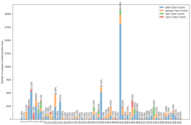
\includegraphics[width=\textwidth]{bilder/ClassCountsPerDatasetAll.png}\centering
		\caption{Class counts for labels in all datasets.}
	\end{subfigure}

	\begin{subfigure}[t]{0.90\hsize}\centering
		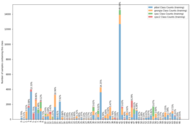
\includegraphics[width=\textwidth]{bilder/ClassCountsPerDatasetTrain.png}\centering
		\caption{Class counts for labels in the training datasets.}
	\end{subfigure}
	\label{fig:ClassCountsBar}
\end{figure}

Since we have multiple possible class labels per patient it might be interesting to see if any of the classes have a correlation to each other. For that we created \autoref{fig:ClassCountsHeatCorrelation} which shows the Pearson correlation coefficient.
%\begin{figure}[H]
%	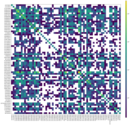
\includegraphics[width=\textwidth]{bilder/ClassOccurences.png}
%	\caption{Logarithmic Class occurrences heatmap: Given class $x$, what other classes $y$ also appear at the same patient?}
%	\label{fig:ClassCountsHeat}
%\end{figure}
\begin{figure}[H]
	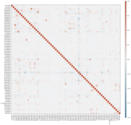
\includegraphics[width=\textwidth]{bilder/ClassOccurencesCorrelation.png}
	\caption{Pearson Class Correlation Coefficient $\rho_{X,Y}$ heatmap: Given class $x$, what other classes $y$ are likely to appear at the same patient?. $\rho_{X,Y}>0=$ positive correlation, $\rho_{X,Y}<0=$ negative correlation, $\rho_{X,Y}\approx 0$ no correlation}
	\label{fig:ClassCountsHeatCorrelation}
\end{figure}


Understanding and classifying ECG data (in real time) using an automated computer system could greatly help the likelihood of surviving an (incoming) infarction, since analysis by eye is time consuming and demands a trained medical professional. Monitoring patients at all times in the hospital could also be a great benefit. While doctors will probably still be mandatory to make the final diagnosis and prescribe medication, an automated classification system that also shows potential highly diagnostic locations in the signal could reduce analysis time by a big factor.



To address the problem of few data being publicly available, solutions different to fully supervised trained models could have a big impact on their success.

One of those more unsupervised learning domains is representation learning.

\subsection{Representation Learning/Background} \label{representation-learning}

In representation/feature learning the algorithm (neural net), tries to learn representations, often in a lower dimension, by not using the real labels directly and instead uses secondary labels extracted from the data itself. After training on these artificial labels, most layers will be used again with their weights to train on the downstream task - the task to predict the desired primary labels. As such representation learning can be split into a pretraining and training phase, which are both needed to produce a working prediction model. The strength of representation learning comes from the fact that unlabeled data is often easier to come by, but which cannot be used by fully supervised methods.

Following Yann LeCun, this is also referred to as self-supervised learning\autocite{YANNLECUNFacebookUnsupervised}, which is partly unsupervised learning since the models do not need the original labels, but there is also an supervisional aspect, where one needs to define secondary labels, related to the downstream task. 

There are many different approaches to representation learning, some train the biggest fraction of the layers using labels that can be extracted with high certainty from the data directly (Jigsaw from image \autocite{noroozi2017unsupervised}, Image Rotation \autocite{gidaris2018unsupervised}, \autocite{doersch2016unsupervised}). Others augment the data and the neural net has to calculate the same lower dimensional representation for both augmented images \autocite{chen2020simple}. 

Another way to learn representation is to predict missing or contextual information, eg. by blacking out known parts of the data and training an algorithm to fill these spots out again. The algorithm will have to find meaningful representations and thus "understand" the data in order predict the missing spots correctly. 

It is hypothesized that solving secondary tasks or predicting contextual information "are fruitful partly because the context from which we predict related values are often conditionally dependent on the same shared high-level latent information" \autocite{DBLP:journals/corr/abs-1807-03748}. That is to say by solving a secondary task and learning representations useful for that specific task, the model will be easier to train on the real problem because the necessary representations are similar to the ones already learned.

Unfortunately the methods mentioned above focus on image recognition and use knowledge not applicable to general sequential data. Also predicting high dimensional data is a very difficult task and simpler loss functions like Mean Squared Error do not work very well. Furthermore architectures like Recurrent Neural Nets that predict only one "step" into the future will likely resort to exploiting "local smoothness" - learning features that only describe the data locally but fail to infer a more global data description.

That's where methods like CPC, short for Contrastive Predictive Coding from the paper "Representation Learning using Contrastive Predictive Coding"\autocite{DBLP:journals/corr/abs-1807-03748} come into play. 

\subsection{Contrastive Predictive Coding}
\subsubsection{Overview}
\label{section:cpcindetail}
The goal of CPC is to learn data representations in a compact (latent) embedding space, which are universally useful in downstream tasks. CPC learns these representations by predicting the future not in the sequential input data, but rather its latent lower dimensional space. Due to the lower dimension, correct predictions of future latents are easier to model. Since there is no ground truth in the unknown embedding space, the architecture is trained with the help of a loss based on Noise-Contrastive Estimation, where the model has to differentiate between latents that stem from the current sample or other samples in the batch.

\begin{figure}[h]
	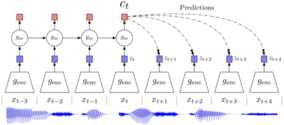
\includegraphics[width=\textwidth]{bilder/Audio-Architecture.png}
	\caption{CPC audio architecture how it is visualized in \autocite{DBLP:journals/corr/abs-1807-03748}}
	\label{cpc-architecture}
	\centering
\end{figure}

\begin{figure}[h]
	\centering
	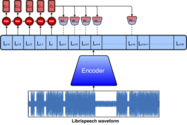
\includegraphics[width=0.8\textwidth]{bilder/CPC-correct-architecture.png}
	\caption{CPC audio architecture how it is visualized in \autocite{lai2019contrastive}}
	\label{fig:cpc-architecture-intersect}
\end{figure}

Both \autoref{cpc-architecture} and \autoref{fig:cpc-architecture-intersect} are CPC architectures, only differing in how the encoder encodes the data into latent representations. They can be used as a close reference for the following description:

First, CPC transforms the sequential data signal $x$ into multiple latent variable vectors $(z_{t-m}\ldots z_t, z_{t+1},\ldots, z_{t+k}, \ldots, z_{t+n})=g_{enc}(x)$ in an embedding space (with potentially lower dimension), using any encoder network. In \autoref{cpc-architecture} $g_{enc}$ encodes parts of the data separately, in \autoref{fig:cpc-architecture-intersect} the Encoder calculates all latents "in one go". $t$ denotes the "current" timestep, $m$ and $n$ are steps into the past and future respectively and may vary depending on chosen architecture/hyperparameters and input data.  The "past" latents $z_{t-m}\ldots z_{t}$ are fed into any recurrent network/autoregressive model (e.g. $g_{ar}$ in \autoref{cpc-architecture}), which produces a context matrix $g_{ar}(z_{t-m}, \ldots, z_{t})=(c_{t-m}, \ldots, c_{t})$, where $c_t$ is the context vector for all seen latents $z_{t-m},\ldots, z_{t}$. Since an autoregressive model is used, any number of latent vectors can be summarized into a context, which can also be sized differently from the latent vectors. The last context $c_t$ is then multiplied individually with $n$ weight matrices $W_1,\ldots, W_n$ to predict $n$ future latent vectors $\hat{z}_{t+1},\ldots, \hat{z}_{t+n}$. Multiple latents are predicted at the same time to counteract the exploitation of local smoothness and force the network to encode globally useful information into the context. In the best case scenario the context represents a meaningful description of all past latents and will be a good feature matrix for following downstream tasks. The disparity between the predicted latents $\hat{z}$ and the latents $z$, produced by the encoder network earlier, can then be used to form the loss and thus train both the encoder and autoregressive model jointly. 

To avoid a trivial encoding of e.g. an all-zero-vector for all latents, a loss based on noise contrastive estimation \autocite{pmlr-v9-gutmann10a} is used, where the network has to differentiate between positive and negative samples. Positive samples are latents that stem from $p(x_{t+k}|c_t)$ --- the same datasource that the context was calculated from. Negative samples are latents that were calculated from $p(x_{t+k})$ --- the unconditioned data distribution, independent from the current context. Negative samples can e.g. be taken from the data batch or in concrete terms another patient.



\subsubsection{Motivation} \label{sec:motivation}
As in \autoref{representation-learning} already said it is assumed that unsupervised representation learning approaches "are fruitful partly because the context from which we predict related values are often conditionally dependent on the same shared high-level latent information" \autocite{DBLP:journals/corr/abs-1807-03748}. With this motivation we want to learn features (latent representations) that maximize the mutual information between the original input and the encoded representations. Mutual information describes how much two probability density functions have in common and how much knowing one leads to knowledge about the other. "More specifically, it quantifies the "amount of information" [...] obtained about one random variable through observing the other random variable". \autocite{MutualinformationWikipedia-2021-03-25}
The equation for mutual information for two probability mass functions is given by \autoref{mutual-information}, where we arrive exactly at the papers definition in the second to last line. Here $x \in X$ are samples from the original signal and $C$ the contexts derived by $x\in X$:
\begin{equation}
	\label{mutual-information}
	\begin{aligned}
		I(X;C)&=\sum_{c\in C}\sum_{x\in X}p_{X,C}(x,c)\log\left(\frac{p_{X,C}(x,c)}{p_X(x)p_C(c)}\right)\\
		&=\sum_{c\in C}\sum_{x\in X}p_{X,C}(x,c)\log\left(\frac{p_{X,C}(x|c)p_C(c)}{p_X(x)p_C(c)}\right)\\
		&=\sum_{c, x}p(x,c)\log\left(\frac{p(x|c)}{p(x)}\right)\\
		&=\EX\log\left(\frac{p(x|c)}{p(x)}\right)
	\end{aligned}
\end{equation}
Mutual Information $I(X; C)$ could thus be described as the mean logarithmic difference between the conditional and the unconditional joint probability distributions of $X$ and $C$. If the conditional probability mass function (PMF) is similar to the unconditional PMF ($\implies X \perp C$), the difference will be close to 0. If the logarithmic difference is bigger, we know that that $X$ and $C$ are conditionally dependent, which means they have a higher Mutual Information.

As our goal, we want to find weights for our model, that \textbf{maximize the mutual information between the input signal $X$ and the calculated context $C$}.

\subsubsection{Math in detail}
To reach our goal, we define the probability that given a context $c_t$ and a set of samples $X$, a specific sample $x_i \in X$ was drawn from the conditional distribution $p(x_{t+k}|c_t)$, rather than from the unconditional distribution $p(x_{t+k})$.
This probability is given by \autoref{eq:pdi} with $[d = i]$ being the indicator that sample $x_i$ is the "positive" sample \autocite[4]{DBLP:journals/corr/abs-1807-03748}:
\begin{equation}
	\begin{aligned}
		p(d=i|X, c_t) &= \frac{p(x_i|c_t)\prod_{l\neq i}p(x_l)}{\sum_{j=1}^{N}p(x_j|c_t)\prod_{l\neq j}p(x_l)} \label{eq:pdi}\\
		&=\frac{p(x_i|c_t)\left(\frac{1}{p(x_i)}\prod_{l=1}^{N}p(x_l)\right)}{\sum_{j=1}^{N}p(x_j|c_t)\left(\frac{1}{p(x_j)}\prod_{l=1}^{N}p(x_l)\right)}\\
		&=\frac{\frac{p(x_i|c_t)}{p(x_i)}}{\sum_{j=1}^{N}\frac{p(x_j|c_t)}{p(x_j)}}\\ 
	\end{aligned}%%&=\frac{p(x_i|c_t)\frac{1}{p(x_i)}}{\sum_{j=1}^{N}p(x_j|c_t)\frac{1}{p(x_j)}}\\
\end{equation}


In \autoref{eq:pdi} the numerator $p(x_i|c_t)\prod_{l\neq i}p(x_l)$ is the probability that $x_i$ was drawn from $p(x_{t+k}|c_t)$, while all other $x_{j}\in X, j\neq i$ were drawn from $p(x_{t+k})$. This gets normalized by $\sum_{j=1}^{N}p(x_j|c_t)\prod_{l\neq j}p(x_l)$, the sum of all probabilities where $x_j$ was drawn from $p(x_{t+k}|c_t)$ instead of $x_i$. Note that $p(x_i|c_t)\prod_{l\neq i}p(x_l)$ is also included in the sum, thus $p(d=i|X, c_t) \in [0,1]$.

The goal of the loss function will be to maximize this probability over all possible combinations between each sample and the corresponding context. Which means the model will need to distinguish between positive and negative samples, given a context. Knowing that the mutual information means: given $C$, how much do we know about $X$, it becomes clear that a model that maximized the mutual information between the original signal and its context, will have an easier "job" to distinguish between real and wrong sample.

The categorical cross entropy loss is a commonly used loss function for training on class probability scores for $N$ classes:
$\sum_{i=1}^{N}y_ilog(\hat{y}_i)$ --- where $y_i$ is the ground truth - and $\hat{y}_i$ is the model prediction.

Combining both the cross entropy loss with \autoref{eq:pdi}, we arrive at the following loss function:
\begin{equation}
	\begin{aligned}
		\mathcal{L_N} &=-\underset{x_i\in X}{\EX}\log\left[\frac{\frac{p(x_i|c_t)}{p(x_i)}}{\underset{x_j\in X}{\sum}\frac{p(x_j|c_t)}{p(x_j)}}\right]
	\end{aligned}
\end{equation}
However, since we cannot evaluate $\frac{p(x_{t+k}|c_t)}{p(x_{t+k})}$ directly, we need a function $f$ s.t. $f_k(x_{t+k}, c_t) \propto \frac{p(x_{t+k}|c_t)}{p(x_{t+k})}$,  ($f$ needs to only be proportional to the optimal value and is not restricted to lay in the interval $[0,1]$). In the paper $f_k(x_{t+k}, c_t) := \exp \left( z_{t+k}^T W_kc_t\right)$ is used to form a simple log-bilinear model. $W_kc_t$ is the models prediction for latent $z_{t+k}$, the dot product between the prediction and the ground truth expresses their similarity, because the dot product between two vectors implies whether they point in the same/opposing/orthogonal direction. This log-bilinear model is also used in the well-known word2vec model in natural language processing \autocite{mikolov2013efficient}.

We thus finally arrive at the InfoNCE loss function from the paper (which can also be described as the logarithmic Softmax over vector similarities): 
\begin{equation}
	\begin{aligned}
		\mathcal{L_N}&=-\underset{X}{\EX}\log\left[\frac{f_k(x_{t+k}, c_t)}{\underset{x_j\in X}{\sum}f_k(x_{j}, c_t)}\right]\\
		&:=-\underset{X}{\EX}\log\left[\frac{\exp \left( z_{t+k}^T W_kc_t\right)}{\underset{x_j\in X}{\sum}\exp \left( z_{j}^T W_kc_t\right)}\right]
	\end{aligned}
\end{equation}

The prove from the original paper, that this loss is indeed maximizing the mutual information between $c_t$ and $x_{t+k}$, is given here with additional steps for easier following (\autoref{eqn:cpc-prove}). For $f_k(x_{j}, c_t)$ it uses the optimal value $\frac{p(x_{t+k}|c_t)}{p( x_{t+k})}$ instead of $\exp \left( z_{t+k}^T W_kc_t\right)$:
\begin{align} \label{eqn:cpc-prove}
	\intertext{Given a set $X$ split into one positive sample $x_{t+k}$ and $N-1$ negative samples $X_{neg}$.}
	\mathcal{L}^{opt}_N &=-\underset{X}{\EX}\log\left[\frac{\frac{p( x_{t+k}|c_t)}{p( x_{t+k})}}{\underset{x_j\in X}{\sum}\frac{p(x_j|c_t)}{p(x_j)}}\right]\\	
	&=-\underset{X}{\EX}\log\left[\frac{\frac{p( x_{t+k}|c_t)}{p( x_{t+k})}}{\frac{p( x_{t+k}|c_t)}{p( x_{t+k})} + \underset{x_j\in X_{neg}}{\sum}\frac{p(x_j|c_t)}{p(x_j)}}\right]\\
	&=\underset{X}{\EX}\log\left[\frac{\frac{p( x_{t+k}|c_t)}{p( x_{t+k})} + \underset{x_j\in X_{neg}}{\sum}\frac{p(x_j|c_t)}{p(x_j)}}{\frac{p( x_{t+k}|c_t)}{p( x_{t+k})}}\right]\\
	&=\underset{X}{\EX}\log\left[\frac{p( x_{t+k})}{p( x_{t+k}|c_t)} \cdot \left(\frac{p( x_{t+k}|c_t)}{p( x_{t+k})} + \underset{x_j\in X_{neg}}{\sum}\frac{p(x_j|c_t)}{p(x_j)}\right)\right]\\
	&=\underset{X}{\EX}\log\left[1 + \frac{p( x_{t+k})}{p( x_{t+k}|c_t)}\underset{x_j\in X_{neg}}{\sum}\frac{p(x_j|c_t)}{p(x_j)}\right]\\
	&=\underset{X}{\EX}\log\left[1 + \frac{p( x_{t+k})}{p( x_{t+k}|c_t)}(N-1)\underset{x_j\in X_{neg}}{\sum}\frac{1}{N-1}\frac{p(x_j|c_t)}{p(x_j)}\right]\\
	\intertext{Assuming all $N-1$ negative samples have approximately the same probability:}
	&=\underset{X}{\EX}\log\left[1 + \frac{p( x_{t+k})}{p( x_{t+k}|c_t)}(N-1)\underset{x_j\in X_{neg}}{\EX}\frac{p(x_j|c_t)}{p(x_j)}\right]\\
	&\approx\underset{X}{\EX}\log\left[1 + \frac{p( x_{t+k})}{p( x_{t+k}|c_t)}(N-1)\right], \text{Assuming $c_t$, $x_j$ are (nearly) independent} \\
	&=\underset{X}{\EX}\log\left[\frac{p( x_{t+k})}{p( x_{t+k}|c_t)}N + 1 - \frac{p( x_{t+k})}{p( x_{t+k}|c_t)}\right]\\
	&\geq\underset{X}{\EX}\log\left[\frac{p( x_{t+k})}{p( x_{t+k}|c_t)}N\right], \text{Assuming $p( x_{t+k}) \leq p( x_{t+k}|c_t)$}\\
	&=-\underset{X}{\EX}\log\left[\frac{p( x_{t+k}|c_t)}{p( x_{t+k})}\right]+\log(N)\\
	&=-I(x_{t+k}, c_t) + \log(N)
\end{align}
Therefore $-I(x_{t+k}, c_t) \geq \log(N) - \mathcal{L}^{opt}_N$, which is also true for loss functions greater than $\mathcal{L}^{opt}_N$ (with non optimal $f \propto \frac{p(x_i|c_t)}{p(x_i)})$. \enquote{Equation (15) quickly becomes more accurate as $N$ increases. At the same time $\log(N)-\mathcal{L}_N$ also increases, so it's useful to use large values of $N$} \autocite{DBLP:journals/corr/abs-1807-03748}.

\subsubsection{Algorithm}
The original CPC Loss formulation can be seen in \autoref{fig:cpcorigloss}.
\begin{tcolorbox}
	\begin{figure}[H]
		\centering
		\caption{"Given a set $X = {x_1, \ldots, x_N }$ of $N$ random samples containing one positive sample from $p(x_{t+k}|c_t)$ and $N - 1$ negative samples from [...] $p(x_{t+k})$, we optimize":}
		\begin{equation}
			\begin{aligned}
				L_N &=-\underset{X}{\EX}\log\left[\frac{f_k(x_{t+k}, c_t)}{\underset{x_j\in X}{\sum}f_k(x_{j}, c_t)}\right]\\
				&:=-\underset{X}{\EX}\log\left[\frac{\exp \left( z_{t+k}^T W_kc_t\right)}{\underset{x_j\in X}{\sum}\exp \left(z_{j}^TW_kc_t\right)}\right] \nonumber
			\end{aligned}
		\end{equation}	
		\subcaption{InfoNCE Loss from \autocite{DBLP:journals/corr/abs-1807-03748}}
		\label{fig:cpcorigloss}
	\end{figure}
\end{tcolorbox}

However we think that this formulation can be misunderstood once it has to be implemented and hence give a mathematical formulation more along the lines of the second paper \autocite{cpcdataefficient}. Note that this version uses every sample $x_i \in X$ once as a positive sample: \autoref{algorithm:cpc-algo}
\RestyleAlgo{boxruled}
\begin{algorithm}[H]
	\caption{InfoNCE Loss calculation}
	\KwData{A set of $N$ \emph{full} data-samples $X=(x_1, \ldots, x_N)$. }
	\tcc{\mycommfont{$X$ can e.g. be a set/batch of patients' ECG records with size $ N \times \mathit{channels} \times \mathit{datalength}$}}
	\KwIn{An index $t\in \mathbb{N}$.}
	\tcc{\mycommfont{$t$ marks the "present" timestep and splits data into "past" and "future". }}
	\KwIn{The encoder network $g_{enc}(x_i|\theta)\mapsto z_i=(z_{i, 1}, \ldots, z_{i, t}, z_{i, t+1}, \ldots, z_{i, t+k})$}
	\tcc{\mycommfont{$z_i$ is a set of $t+k$ latent vectors, representing consecutive timesteps of the input data in a lower dimension. How many get produced is dependent on the encoder network and data samples $x \in X$}}
	\KwIn{The context network $g_{ar}((z_{i, 1}, z_{i, 2}, \ldots, z_{i, t})|\psi) \mapsto c_{i,t}$}
	\tcc{\mycommfont{$c_{i,t}$ is the context vector for a set of $t$ latent vectors, for data-sample $x_i$}}
	\KwIn{A set of $n$ weight matrices $\{W_1 \ldots W_n$\}}
	\tcc{\mycommfont{The weight matrices are used to calculate a set of $n$ latent vectors} $\hat{z}_{i}=(\hat{z}_{i, t+1}, \ldots, \hat{z}_{i, t+n}) := (W_1c_{i, t}, W_2c_{i, t}, \ldots, W_nc_{i, t})$}
	\KwResult{
	\begin{flushleft}		
		\[\mathit{Loss}_i := -\frac{1}{k}\sum_{k=1}^{n}\log\left[\frac{\exp(\hat{z}_{i, t+k}^Tz_{i, t+k})}{\exp(\hat{z}_{i, t+k}^Tz_{i, t+k})+\underset{{(j,l)\in \{(j,l)|j\neq i \land l \leq |z_i|\}}}{\sum \exp(\hat{z}_{i, t+k}^Tz_{j, l})}}\right]\]
		\tcc{\mycommfont{$\mathit{Loss}_i$ is the scalar loss value for a single positive data-sample $x_i$. This is close to the papers definition.}}
		
		\[\mathit{Loss} := \frac{1}{N}\sum_{i=1}^{N}\mathit{Loss}_i=\]
		\[=-\frac{1}{kN}\sum_{i=1}^{N}\sum_{k=1}^{k}\log\left[\frac{\exp(\hat{z}_{i, t+k}^Tz_{i, t+k})}{\exp(\hat{z}_{i, t+k}^Tz_{i, t+k})+\sum_{(j,l)\in \{(j,l)|j\neq i \land l \leq |z_i|\}}\exp(\hat{z}_{i, t+k}^Tz_{j, l})}\right]\]
		\tcc{\mycommfont{$\mathit{Loss}$ is the scalar loss value where each data-samples $x_i\in X$ is the positive sample once.}}
	\end{flushleft}}
	\label{algorithm:cpc-algo}
\end{algorithm}
Note that the set of negative latent samples $A:=\{(j,l)|j\neq i \land l \leq |z_i|\}$ can be replaced by e.g. $A_1\subset\{(j,l)|j\neq i \land l \leq |z_i|\} \leftrightarrow A_1 \textit{ is a random subset of }A$, if there are too many negative samples for the hardware to handle, or by e.g.
$A_2:=\{(j,l)|j\neq i \land l = t+k\}\leftrightarrow A_2 \textit{ is only using negative examples that share the same timestep as }z_{i, t+k}$, to provide samples that might be more similar to the positive one.

Furthermore we provide an algorithm in Python pseudo code from our understanding, to further explain the loss function and clear up potential confusion. \autoref{algo:cpcslow} shows this pseudo code for a naive implementation of the formula we provided in \autoref{algorithm:cpc-algo} (with negative samples that stem from other batches but the same timestep).
\begin{minipage}{\linewidth}
\begin{lstlisting}[language=Python, caption=Naive CPC Loss Pseudo Code, label=algo:cpcslow]
def cpc_loss_naive(X:Tensor, W:List[Tensor], enc:nn.Module, rnn:nn.Module):
	batch, channels, data_length = X.shape #eg. (64 x 12 x 4500)
	#Encode data into latents:
	latent_matrix = enc(X)
	batch, timesteps, latent_size = latent_matrix.shape #eg. (64 x 27 x 128)
	#Calculate context from latents:
	context_matrix = rnn(latent_matrix)
	batch, timesteps, context_size = context_matrix.shape #eg. (64 x 27 x 256)
	#Select current timestep (here last possible):
	n=len(W)
	current_timestep = timesteps-n-1
	last_context_vector = context_matrix[:, current_timestep, :]
	#output shape: (64 x 256)
	loss = 0.        
	for i in range(batch):
		loss_i = 0.    
		for k in range(n):
			#Predict latent for specific timestep k from current context:
			latent_vector_pred_i = last_context_vector[i] @ W[k]
			#Select latent vector for batch i at correct timestep:
			latent_vector_i = latent_matrix[i, current_timestep+k+1, :] 
			#calculate similiarity with dot product:
			sim = latent_vector_pred_i @ latent_vector_i #scalar
			#calculate exp(sim) for softmax
			p_xi_ct = exp(sim) 
			nominator = p_xi_ct
			denominator = 0.
			for j in range(batch): #replace j with j, l for different sampling
				latent_vector_j = latent_matrix[j, current_timestep+k+1, :] 
				#Calculate dot product to measure similarity:
				sim = latent_vector_pred_i @ latent_vector_j #scalar
				#Calculate exp(sim) for softmax
				p_xj_ct = exp(sim) 
				denominator += p_xj_ct
			#take log for log softmax
			loss_i += log(nominator/denominator)
		loss += -loss_i/n
	return loss / batch
\end{lstlisting}

\end{minipage}

\begin{minipage}{\linewidth}
	\begin{lstlisting}[language=Python, caption=Optimized CPC Loss Pseudo Code. Uses CrossEntropyLoss from Pytorch, label=algo:cpcfast]
def cpc_loss_fast(X:Tensor, W:List[nn.Module], enc:nn.Module, rnn:nn.Module):
	
	batch, channels, data_length = X.shape #eg. (64 x 12 x 4500)
	
	latent_matrix = enc(X)
	batch, timesteps, latent_size = latent_matrix.shape #eg. (64 x 27 x 128)
	
	context_matrix = rnn(latent_matrix)
	batch, timesteps, context_size = context_matrix.shape #eg. (64 x 27 x 256)
	
	timesteps_out = len(W) #eg. 12
	current_timestep = timesteps-timesteps_out
	last_context_vector = context_matrix[:, current_timestep-1, :] #shape: (64 x 256)
	loss = 0.
	accuracy = 0.
	for k in range(timesteps_out):
		#predict latents for timestep k and all items in batch:
		pred_latent = W[k](last_context_vector) #shape: (64 x 128)
		#calculate similarity between all encoded latents against pred_latent:
		sim = latent_matrix @ pred_latent.T #shape eg.: (64 x 27 x 64)
		#reshape result for easier/efficient indexing:
		sim_r = sim.reshape(timesteps*batch, batch).T #shape eg.: (64, 1728)
		#Select the indices where pred_{i,k}==latent_{i,k}
		labels = torch.arange(batch) + batch*(current_timestep + k)
		#pytorch: crossentropyloss = LogSoftmax + NLL_Loss
		loss += crossentropyloss(sim_r, labels)
		#Count how often the max softmax value is at the correct idx
		accuracy += (sim_r.max(dim=-1).indices == labels).sum()
	
	loss = loss / (timesteps_out*batch)
	accuracy = accuracy / (timesteps_out*batch)  # * pred_latent.shape[0]
	return accuracy, loss, hidden
	\end{lstlisting}

\end{minipage}

%\input{hauptteil}
\section{Implementation}
In this section we describe our different models and their implementational details. All code is available at our github repository\footnote{\url{https://github.com/Lullatsch/ecg-cpc}}.

\subsection{CPC}
Since CPC is a \enquote{self-supervised} architecture, there are different parts of the network that are used according to the current task. The pretraining architecture without labels is described in \autoref{sec:cpc-unsupervised}. The downstream training architecture is described in \autoref{sec:cpc-supervised}.

\subsubsection{Unsupervised}\label{sec:cpc-unsupervised}
CPC was implemented following the original paper \autocite{DBLP:journals/corr/abs-1807-03748} with focus on the section "3.1 Audio", which uses CPC as a speaker and phone classification method on the librispeech dataset. Since audio data is also sequential and thus comparable to ECG data, the architectural details were a good starting point. We adopted the encoder network with only small changes, which means we use 5 convolutional layers with kernel-sizes $[10, 8, 4, 4, 4]$, strides $[5, 4, 2, 2, 2]$ and ReLU activations in between, directly on the input data. The amount of channels is set to $128$ after the initial $12$. This is different from the original paper \autocite{DBLP:journals/corr/abs-1807-03748} where $512$ "hidden units" are used instead. This means that each latent vector has the length $l_{size}=128$. The latents are calculated \enquote{in one go}, which means for this architecture and a data input with dimensions $\mathit{batch} \times 12 \times 4500$, a latent matrix sized $\mathit{batch} \times l_{size} \times t_{total} = \mathit{batch} \times 128 \times 26$ is calculated. The total number of latent timesteps $t_{total}=26$ is directly given by the architecture and input data length. The transposed encoder output/latent matrix is fed into a GRU model with a hidden state dimension of $256$ to form the models context for each of the columns in the latent-matrix, resulting in the context-matrix of shape $\mathit{batch} \times 26 \times 256$. In theory, since a recurrent network is used for its calculation, each context vector in the context-matrix can represent a summary or state of the prior latent vectors. From a selected column $t$ in the context-matrix, $t_{out}=12$ individual linear/fully-connected layers are used to predict $t_{out}=12$ latent vectors into the future. The value of $t$ should not be selected to low, as a meaningful context, from which can be predicted correctly, requires multiple latents. In our case, we select the latest possible context vector $t=t_{total}-t_{out}=26-12=14$th timestep, which is also the most interesting context entry, since it encodes all seen latents. Note that you can also make the $t_{out}=12$ predictions from every possible column $\{t | t_{in}\leq t \leq t_{total}-t_{out}\}$ in the context matrix in one forward pass, to make more use of the input data, however this comes at the cost of training time. $t_{in}$ eg.$=12$ is newly introduced additional hyperparameter which defines how many latent vector are at least used to encode the context. A randomly selected timestep from the set $\{t | t_{in}\leq t \leq t_{total}-t_{out}\}$ is another possibility which we used. 

Now with the encoded and predicted latent values only, the CPC-loss can be drawn.

Like in the introduction already mentioned the CPC loss uses a modified noise contrastive estimation loss called \textit{InfoNCE}. Here the negative samples are other ECG files drawn from the batch. We differentiate between the latent sets $A=\{z_{j,l}|j\neq i \land l\in[1, |z_j|]\}$ (all latents including past and future from other patients) and $A_2=\{z_{j,l}|j\neq i \land l = t+k\}$ (only latents from other patients at the same timesteps) as negative examples. The details on the loss are explained in algorithm \autoref{algorithm:cpc-algo}, \autoref{algo:cpcslow}, \autoref{algo:cpcfast} or in \autoref{section:cpcindetail}.

\subsubsection{Supervised}\label{sec:cpc-supervised}
For the downstream task, the InfoNCE-loss function is not used anymore. Nevertheless the whole network that calculates latent-, context- or future latent-vectors will still be used. In the original paper \autocite{DBLP:journals/corr/abs-1807-03748}, a single linear layer is used on the last context vector in conjunction with a multi-class linear logistic regression classifier to predict the data labels. We applied multiple different architectures to the models output; for a full list see section \autoref{sec:cpc-downnetwork}

\subsection{CPC with modifications}
Apart from the model described above, additional architectures similar to the CPC audio architecture were examined with changes to different parts of the network.

\subsubsection{Loss calculation changes}
\paragraph{Latent sampling}
As already mentioned (see right sum in denominator of \autoref{algorithm:cpc-algo}) there are multiple possibilities as to what negative samples (other latent vectors) are compared to the "current" latent prediction:
$N = \mathit{batch\ size}, t=\mathit{total\ timesteps}, t_{out}=\mathit{number\ of\ predicted\ timesteps}$
\begin{itemize}
	\item[\underline{same}] uses all latent vectors from the same timestep as the predicted latent vector in the batch. The model has thus to recognize one value under $N$ values for each predicted timestep, for all items in the batch $=N^2*t_{out}$ total guesses.
	\item[\underline{future}] uses all latent vectors from future timesteps in the loss calculation. The model has to recognize the correct latent value under $N*t_{out}$ values for each predicted timestep, for all items in the batch $=N^2*t_{out}^2$ total guesses.
	\item[\underline{all}] uses all latent vectors from all available timesteps in the loss calculation. The model has to recognize the correct latent value under $N*t$ values for each predicted timestep, for all items in the batch $=N^2*t*t_{out}$ total guesses. In the results this method is the same as \underline{crossentropy} which just uses a slightly different implementation and is always used in conjunction with "Fewer Latent Vectors" (\autoref{sec:fewerlatentvectors}).
\end{itemize}

\paragraph{Fewer latent vectors}\label{sec:fewerlatentvectors}
One handicap we came across during training is that with many latent vectors, which might get generated for long input sequences or an encoder architecture with a lower downscaling factor, the loss calculation takes a long time because the model has to calculate big dot product matrices and the softmax afterwards, which is a costly operation. Furthermore recurrent architectures tend to consume large amounts of memory for long input sequences which even made training impossible altogether in some cases.

As a solution we limited the latents which are to be used in the loss calculation to a fixed number, instead of trying to use all latent vectors. During Downstream training, all data is used again, which allows for a more representative context matrix and is important for correct classification. The network is called \code{cpc\_intersect\_manylatents} (because it "deals with" many latents), as opposed to the standard architecture \code{cpc\_intersect}.

\paragraph{Normalized latent vectors}\label{sec:normalizedlatents}
We test normalizing the latent vectors $z$ and $\hat{z}$ to unit vectors (length is $1$), before their multiplication in the loss to receive scalar values in range [-1, 1], instead of an open interval. As a result we can observe the following properties:
\begin{enumerate}
	\item If $z*\hat{z} = 1 \implies z$ and $\hat{z}$ are parallel and point in the same direction.
	\item If $z*\hat{z} = 0 \implies z$ and $\hat{z}$ are orthogonal.
	\item If $z*\hat{z} = -1 \implies z$ and $\hat{z}$ are parallel and point in the opposite direction.
\end{enumerate}
We justify this change because higher valued latent vectors that are not calculated from the current context, but still point in the generally same direction, might be falsely classified as the positive sample. Note that during downstream tasks, we tested both to return the un-normalized calculated latents and the unit vectors, where returning the normalized vectors worked better by a margin. The loss function thus becomes:
\begin{equation}
	\mathit{Loss}_i := -\frac{1}{k}\sum_{k=1}^{n}\log\left[\frac{\exp(\frac{\hat{z}_{i, t+k}}{\|\hat{z}_{i, t+k}\|}^T\frac{z_{i, t+k}}{\|z_{i, t+k}\|})}{\exp(\frac{\hat{z}_{i, t+k}}{\|\hat{z}_{i, t+k}\|}^T\frac{z_{i, t+k}}{\|z_{i, t+k}\|})+\underset{{(j,l)\in \{(j,l)|j\neq i \land l \leq |z_i|\}}}{\sum \exp(\frac{\hat{z}_{i, t+k}}{\|\hat{z}_{i, t+k}\|}^T\frac{z_{j, l}}{\|z_{j, l}\|)}})}\right]
\end{equation}
To circumvent an erroneous division by $0$ and the loss becoming undefined, we clip all vector lengths to be in the interval $[\epsilon, \infty]$, where $\epsilon$ is a constant scalar (we chose $1e-6$):

$\|z\|^*=
\begin{cases}
	\|z\|,& \text{if } \|z\| > \epsilon\\
	\epsilon,& \text{else}\\
\end{cases}$

%We additionally tried instead of clipping:
%\begin{equation}
%	\mathit{Loss}_i := -\frac{1}{k}\sum_{k=1}^{n}\log\left[\frac{\exp(c\cdot\frac{\hat{z}_{i, t+k}}{\|\hat{z}_{i, t+k}\|}^T c\cdot\frac{z_{i, t+k}}{\|z_{i, t+k}\|})}{\exp(c\cdot\frac{\hat{z}_{i, t+k}}{\|\hat{z}_{i, t+k}\|}^T c\cdot\frac{z_{i, t+k}}{\|z_{i, t+k}\|})+\underset{{(j,l)\in \{(j,l)|j\neq i \land l \leq |z_i|\}}}{\sum \exp(c\cdot\frac{\hat{z}_{i, t+k}}{\|\hat{z}_{i, t+k}\|}^T c\cdot\frac{z_{j, l}}{\|z_{j, l}\|)}})}\right]
%\end{equation}

However in practice our model scores in the result section got slightly downgraded by normalizing the latent vectors. We suspect that although having access to the properties of comparing unit vectors, this change also restricted the model, hurting classification accuracy.

\subsubsection{Encoder networks}
The encoder architecture from the paper produces $26$ latent vectors for data with length $4500$. There one cannot control how many latent vectors get produced, besides changing the encoder architecture or varying data length. Since each latent vector is calculated from at least $465$ datapoints, which can be calculated by transposing the convolutions in the architecture, and each vector represents a window shifted by $5*4*2*2*2=160$ (product of strides, or the downsampling factor given in the original paper), this is equal to an overlap of $\frac{465-160}{465}=\frac{305}{465}\approx\frac{2}{3}$ in the data for neighboring vectors, making the exploitation of local smoothness in the next step prediction likely. Furthermore we would like to point out that the statement from the paper: \enquote{The total downsampling factor of the network is 160 so that there is a feature vector for every 10ms of speech}, is ambiguous, since it conveys the impression that one latent vector is being created from 10ms of audio. In reality one latent vector is being calculated from 465 data points $\frac{465}{16000\mathit{hz}}*1000\approx29\mathit{ms}$ rather than from $\frac{160}{16000\mathit{hz}}*1000=10\mathit{ms}$. It would be more correct to say that one latent vector is calculated from $\frac{465}{16000\mathit{hz}}*1000\approx29\mathit{ms}$ of audio, with an overlap of $\frac{305}{16000\mathit{hz}}*1000\approx19\mathit{ms}$, creating an additional non disjoint latent vector after every $\frac{160}{16000\mathit{hz}}*1000=10\mathit{ms}$.
\paragraph{Data sliding window} \label{sec:cpc-strided}
We compare the original "intersecting" model to a different encoder network that encodes the data by breaking it into multiple non-overlapping windows and then encodes each separately. This ensures that the autoregressive model has to predict future latent vectors which are not calculated from partly identical data and thus have to learn non-local features that do not exploit "local smoothness". Additionally the differentiation between positive and negative samples should be a lot harder too, improving the latent representations. In detail that means an input array of size $\mathit{batch} \times \mathit{channels} \times \mathit{length}$ is split into a fixed number e.g. $M \times \mathit{batch} \times \mathit{channels} \times \frac{\mathit{length}}{M}$ of non-overlapping windows, which are then encoded into $M \times \mathit{batch}$ latent vector. The model is called \enquote{strided} in the results and \code{cpc\_encoder\_as\_strided} in the code, where it acts as a module wrapper applicable to every encoder network.

%This might be possible to counteract by \emph{not} predicting the next $1, ..., n$ steps, but rather the next $a, ..., n$ for $a\geq2$ or, like in the paper mentioned but not applied, using masked convolutional layers, which could "black-out" values already seen by previous iterations. 

One downside is that the window-size $\frac{length}{M}$ needs to be fixed or more specifically for an input with dimensions $batch \times channels \times \frac{length}{M}$ the architecture needs to produce exactly $batch \times latentsize \times 1$ values. This can be easily solved with mean pooling or similar methods but not relying on those techniques may yield more accurate results. 
Furthermore, using the same encoder as in the original architecture, due to no data overlap, we produce less latent vectors which becomes a problem for small data lengths. Using different encoders that can deal with smaller input sizes than $465$ would solve this data restriction.
\paragraph{Baseline-like Network}
To evaluate whether potential downstream task performance differences were stemming from architecture distinctions rather than the special CPC pretraining, we used the good working baseline architecture \code{baseline\_v8} (explained later) as an encoder network, called \code{cpc\_encoder\_likev8}. It comes with the property of reducing less values from the input data, making the output larger which can be useful if the data contains many information or if a larger output is needed for following tasks. One difficulty that arises due to the smaller downsampling factor in comparison to the standard cpc encoder, is that more latent vectors are created, which in turn leads to heavily inflated training durations, mostly because of the latent sampling method. Additionally recurrent architectures sometimes fail to cope with very long input sequences. The issue was solved by combining this encoder network with a different architecture that uses a fixed-size subset of latent vectors, already explained in \autoref{sec:fewerlatentvectors}, returning in fewer latents during the loss calculation.

\subsubsection{Context prediction networks}
In the original paper a GRU model is used to summarize all latent vectors prior to the current timestep into a context vector. We assume that, in the paper, the output for each latent vector is meant with "model output" and took the last output as the context. In contrast to that we implemented a network which uses the hidden state as context and predicts the future latent values from there. Since the hidden state is internally used to calculate the autoregressive model output, it should contain a lot of information about past latents, which makes it a good candidate for next-step latent prediction as well. It is called \code{cpc\_autoregressive\_hidden} in the code.

\subsubsection{Latent prediction networks}
Originally CPC uses a fixed number of simple weight matrices/ single linear layers to predict future latents from the current context. Next to this predictor which internally uses $12$ linear layers to predict $12$ latent vectors, called \code{cpc\_predictor\_v0}, we additionally implemented a predictor that completely eliminates the use of an autoregressive context network by directly predicting future latent vectors from past latents. For this we used a Temporal Convolutional Network \autocite{bai2018empirical}, which is a convolutional many-to-many sequence architecture we also used as one of our baselines (see Baseline \autoref{sec:literature-arch}). As a result, no pretrained context matrix is available in downstream-training, but we relief the model from first summarizing latent values and then secondly applying a number of linear layers synchronously.

\subsubsection{Downstream task networks}\label{sec:cpc-downnetwork}
For each ECG sample, CPC calculates latent vectors with the encoder model, and a context vector with the autoregressive model. Although both can be used for classification later on, it is easier to use the context vector because only one is getting calculated no matter the ECG signal length. Nevertheless if we use the latent vectors during downstream training, to account for varying dimensions, latents have either been flattened, summarized with a new autoregressive architecture, or pooled to obtain a single dimension for prediction with linear layers. The output of the networks is then activated with a sigmoid function. We differentiate between multiple network-types:
\begin{itemize}
	\item \underline{Single Linear Layer + Pooling} In the original paper, to test the capabilities of CPC, a single linear layer was used on the latent vectors. However since our input size might change we used a pooling operation to condense multiple latents into one feature vector. Afterwards we apply a linear layer to the output. Because the context vector was used to predict future latents, it should contain enough information about the data for classification. As a result we can use the context vector as a feature vector too, which we do by feeding it to a linear layer. If both latents and context are desired, we add both together to form the output, before a sigmoid activation is used. This model is called \code{cpc\_downstream\_only} in the results.
	\item \underline{Single Conv. Layer + RNN} Following works that omit linear layers completely, we also test a single convolutional layer that predicts the output classes in the channel dimension. If latents are used in the prediction we summarize latents with an additional GRU with hidden size $256$. If both latents and context are used in downstream training the values are concatenated, instead of added. (\code{cpc\_downstream\_cnn} in the results.)
	\item \underline{Linear Layer + Pooling} In this network we make class prediction for all latents with a single linear layer. To obtain the final result we simply take the maximum value across the data dimension for each of the separate classes. If the context is used a single linear layer is used on the context vector. If both latents and context are used we simply add both outputs together before calculating the sigmoid activation. The model \code{cpc\_downstream\_latent\_maximum} uses the maximum pooling operation. The idea behind this network is that each latent might include some class that is supposed to be propagated into the final result with the maximum pooling, no matter how often the class appears. The model \code{cpc\_downstream\_latent\_average} applies an average pooling operation instead, which makes classes that appear in the data at multiple locations more likely to be considered true in the final probability output.
	\item \underline{2 Linear Layers + RNN} If the predicted classes are not linearly separable from context and latents, additional layers have to be used. We examined two stacked linear layers with ReLU activation in between. Again, when latents are used, they are summarized with a GRU network with hidden size $256$. If both context and latents are used they are stacked together and then forwarded through the two linear layers. (\code{cpc\_downstream\_twolinear} in the code)
	\item \underline{2 Linear Layers + Max Pool} In addition to the 2 linear layers above, we also used an identical network with the difference that latents are maximum pooled instead, and latents and context are added instead of stacked, after they have been feed through the linear layers. (\code{cpc\_downstream\_twolinear\_v2} in the code)
\end{itemize}
We decided against using deeper, more powerful models, as we want to focus on the latent representations learnt during pretraining, rather than finding the theoretically best performing model in general.
\subsection{Baselines}
We implemented different fully supervised models to compare the CPC-models' performance on the ECG data.

\subsubsection{Custom baseline architectures}
Multiple hand crafted fully supervised convolutional architectures were examined, each with slight modifications to test for the best performance.  

The different baseline architectures were build to have different sets of the following parameters:
\begin{description}
	\item \underline{Number of Convolutions}: Two up to six stacked layers of one dimensional convolutional layers have been tested
	\item \underline{Use of BatchNorm}: We tried if including a BatchNorm\autocite{ioffe2015batch} layer after each Convolution helps training and found that it slightly sped up convergence but since we trained for a fixed set of epochs this benefit was negligible
	\item \underline{Strides}: We found that using strides $>1$ in early network layers improved accuracy and lead to better performance in most networks.
	\item \underline{Pooling}: Different Pooling operations have been tried either between all layers, or at the end of the network. Namely Global Average Pooling (AdaptivePooling with output size 1), Maximum and Average Pooling with different kernelsizes. 
	\item \underline{Dilation}: We used dilation in different layers. As argued in the TCN paper \autocite{yu2016multiscale} dilated convolutions can build big receptive fields in a short number of layers (receptive field is exponential to number of layers) making it ideal for our ECG data.
	\item \underline{Kernel size}: Different kernel sizes were experimented with ranging from 3 to 12 (or 1 in special cases). We observe that using bigger kernelsizes in early layers helped accuracy.
	\item \underline{Final output Layer}: We applied a linear layer to the convolutional network output (filter output map), in order to calculate scores for all the diagnostic classes. However multiple approaches have been taken to reshape the network output of shape $(N, C, L) := (\mathit{batch} \times \mathit{convchannels} \times \mathit{datalength})$
	\begin{enumerate} \label{desc:enum}
		\item \label{desc:en1} Flatten the tensor to receive a shape of $(N, C*L)$
		\item \label{desc:en2} Take only the last value in the data dimension to receive a shape of $(N, C, 1)$
		\item \label{desc:en3} Use a global pooling (mean or max) operation to receive a shape of $(N, C, 1)$
		\item \label{desc:en4} Use an additional convolutional layer  with $L$ input channels, an output channel of $1$ and a kernel size of $1$, on the last dimension of the transposed data to receive a shape of $(N, C, 1)$
		\item \label{desc:en5} Use a recurrent architecture to summarize the values in the last dimension by outputting a vector at each step and taking the last as context, to receive a shape of $(N, C, 1)$		
	\end{enumerate}
\end{description}
Although \ref{desc:en1} seems like a good idea because no information is lost, the accuracy was low when $L$ was large and the weight matrix for the linear layer gets substantially bigger, resulting in longer training times, higher memory requirements and a harder training process.
Option \ref{desc:en2}  is the least taxing operation, however a lot of information is lost in the process which also reflected in a lowered accuracy.
Option \ref{desc:en3}  does not introduce new parameters and worked approximately as good as option \ref{desc:en2}.  However the bigger the filter output map, the worse the network performed in general.
Option \ref{desc:en4}  performed the best by a margin, but also introduced new parameters since a new weight matrix for the filter has to be learned. However we opt to still use this option because it is more expressive and can even learn both option \ref{desc:en2} or \ref{desc:en3}, if desired. Furthermore convolutions with a 1x1 kernel (1 in our case because of data dimension) are widely used as a downsampling measure and are established in many models.
Option \ref{desc:en5}  can be compared to the CPC architecture, however when trained supervised end-to-end this method did perform poorly. We suspect that the partly large values for $L$ make it difficult to train recurrent architectures.

While we think that there are many possible approaches to summarizing the last layers output, the best solution might be to choose architectures that obtain small values for $L$.

Most models follow a general structure: 

Multiple one-dimensional Convolution Layers with decreasing kernel sizes and either stride or dilation, get stacked with ReLU after each Layer. Batchnorm is added to some models. The first few layers of the network are supposed to downsample the data using big kernel sizes and strides, reducing memory footprint for the model drastically. After the downsampling layers, additional one-dimensional convolutional layers have been used, this time with a mostly fixed kernel size of 3, low or no strides and no or increasing dilation, which increase the networks receptive field, potentially extracting wide spanning features. The number of filters is increased from 12 to 128 to allow enough features to be learned by the model. The filter number has been kept constant at 128, which is unusual but since we had differing layer numbers we opted for a simple solution. Finally the non-channel dimension has been summarized by a one of the techniques described in \hyperref[desc:en1]{\underline{Final output Layer}}. The resulting data of shape (Batch-size, 128, $1$) is fed into a fully connected or convolutional layer with sigmoid as activation function, to predict class labels with probability scores $\in [0, 1]$ each. Note that Softmax is not used as the probabilities do not add up to $1$ in multi-label classification. 

Table \ref{table:modelattributes} summarizes most of the differing model attributes described above. The model names are the same as in the results.


Because the summary table can not fully capture all details of the different models, we will briefly describe our baseline models here, that either do not fit the above general description or get used often:
\begin{itemize}
	\item[\code{BL\_v0}] 2 one-dimensional convolutinal layers, with kernel-sizes $[7,3]$, dilations $[1, 3]$ and ReLU activations. The output is summarized by a convolutional with kernel size 1 (option \ref{desc:en4}).
	%\item[\code{BL\_v0\_1}] Similar to \code{BL\_v0} but additionally uses strides $[2, 1]$.
	\item[\code{BL\_v0\_2}] consists of 5 Conv1D Layers with kernel sizes of $[7,5,5,3,3,3]$, dilations of $[1,1,1,1,2,4]$, strides $[4,3,3,1,1,1]$ and ReLU inbetween. The channel number is dropped down to $32$ in the first layer with stride $1$, and then increased back up to $64$. The idea behind this network is to downsample the input in the first few layers and then extract spanning features with dilations without striding.
	\item[\code{BL\_v2}] \code{BL\_v2}, consists of 5 Conv1D Layers with kernel sizes of $3$ and dilations of $[1,2,4,8,16]$, the channel size is $128$ after the initial $12$. BatchNorm and ReLU is applied after each layer. At the end of each besides the last layer a maximum pooling layer with filter size $3$ is used. The output is summarized with a global average pool like option \ref{desc:en3} describes.
	%\item[\code{BL\_v7}] 5 convolutional layers with ReLU activations in between and a (TODO)
	\item[\code{BL\_v8}] Similar to \code{BL\_v2} but smaller, \code{Baseline\_v8} consists of 4 Conv1D Layers with kernel sizes of $3$ and dilations of $[1,2,4,8]$, the channel size is $128$ after the initial $12$. BatchNorm and ReLU is applied after each layer. At the end of each besides the last layer a maximum pooling layer with filter size $3$ is used. The output is downsampled in the data dimension like option \ref{desc:en4} describes. 
%	\item[\code{BL\_v15}] Similar to \code{BL\_v8}, but uses dilations of $[1,7,21,63]$ instead, resulting in a much smaller output size.
	%TODO add some? or all?
\end{itemize}


\subsubsection{Literature architectures} \label{sec:literature-arch}
In addition to the custom-designed architectures above, we tested already existing or slightly modified architectures that were reported to work on timeseries classification:
\begin{description}
	\item [MLP] The Multi-Layer-Perceptron is a three linear layer network with dropout and ReLU activations from \autocite{strongbaseline} (\code{BL\_MLP} in results)
	\item [FCN] The Fully Convolutional Network consists of three convolutional layers with BatchNorm, ReLU and a global pooling operation from \autocite{strongbaseline}. (\code{BL\_FCN} in results)	
	\item [Multi Scale 1D ResNet] A Residual Network which uses one instead of two dimensional convolutions, tuned for timeseries classification \autocite{githubmultiscale}. Multiple subarchitectures are used in parallel to allow for modeling close and long distance coherence in sequential data. Each subarchitecture uses different filter sizes and striding to produce local or global features at the same time. (\code{BL\_v14} in results.)
	\item [TCN] Temporal Convolutional Networks \autocite{bai2018empirical} aim to provide an almost fully convolutional sequence-to-sequence alternative to RNNs, which brings perks like low memory requirements, more stable gradients and parallelism (predicting many timesteps at once). Exponentially increasing dilation sizes help in building a big receptive field, theoretically ideal for modeling long distance coherence in sequential data. (\code{BL\_TCN} in results)
	Since this model's output has the same length as the models input, we had yet again to find a solution to reduce the output length and tested multiple variants:
	\code{TCN\_down} uses a convolutional layer with filter-size 1 to reduce output. \code{TCN\_last} uses the last value in the output of the data dimension, following one of the examples in the authors github repository \footnote{https://github.com/locuslab/TCN/tree/master/TCN/mnist\_pixel}
	\item[Alexnet] The Alexnet is an architecture known for image classification. Here we implemented it with 1D convolutions and two different kernel sizes otherwise following the implementation from pytorch \autocite{visionalexnetpyatmasterpytorchvision-2021-06-26}.	(\code{BL\_alex\_v2} in the code)
\end{description}

Again, Table \ref{table:modelattributes} summarizes most model attributes described above.

\begin{table}
	\rotatebox{90}{
		\resizebox{1.0\textheight}{!}{
			\begin{tabular}{lrrrrrllllll}
{} & {Convolutional Layer Number} & {Sum of Strides} & {Sum of Dilation} & {Sum of Paddings} & {Sum of Filters} & {uses BatchNorm} & {uses Max Pool} & {uses Adaptive Average Pooling} & {uses Linear} & {uses LSTM} & {Final Layer} \\
{Model Name} & {} & {} & {} & {} & {} & {} & {} & {} & {} & {} & {} \\
BL\_alex\_v2 & {\cellcolor[HTML]{C2DFC2}} \color[HTML]{000000} 5 & {\cellcolor[HTML]{98CA98}} \color[HTML]{000000} 25 & {\cellcolor[HTML]{D7E9D7}} \color[HTML]{000000} 8 & {\cellcolor[HTML]{CDE5CD}} \color[HTML]{000000} 7 & {\cellcolor[HTML]{008000}} \color[HTML]{F1F1F1} 174 & no & yes & yes & yes & no & 1 \\
BL\_FCN & {\cellcolor[HTML]{D3E7D3}} \color[HTML]{000000} 3 & {\cellcolor[HTML]{E1EEE1}} \color[HTML]{000000} 3 & {\cellcolor[HTML]{E3EFE3}} \color[HTML]{000000} 3 & {\cellcolor[HTML]{EBF3EB}} \color[HTML]{000000} 0 & {\cellcolor[HTML]{D5E9D5}} \color[HTML]{000000} 16 & yes & no & no & no & no & 3 \\
BL\_MLP & {\cellcolor[HTML]{EBF3EB}} \color[HTML]{000000} 0 & {\cellcolor[HTML]{EBF3EB}} \color[HTML]{000000} 0 & {\cellcolor[HTML]{EBF3EB}} \color[HTML]{000000} 0 & {\cellcolor[HTML]{EBF3EB}} \color[HTML]{000000} 0 & {\cellcolor[HTML]{EBF3EB}} \color[HTML]{000000} 0 & no & no & no & yes & no & 2 \\
BL\_rnn\_simplest\_lstm & {\cellcolor[HTML]{EBF3EB}} \color[HTML]{000000} 0 & {\cellcolor[HTML]{EBF3EB}} \color[HTML]{000000} 0 & {\cellcolor[HTML]{EBF3EB}} \color[HTML]{000000} 0 & {\cellcolor[HTML]{EBF3EB}} \color[HTML]{000000} 0 & {\cellcolor[HTML]{EBF3EB}} \color[HTML]{000000} 0 & no & no & no & yes & yes & 5 \\
BL\_TCN\_block & {\cellcolor[HTML]{D3E7D3}} \color[HTML]{000000} 3 & {\cellcolor[HTML]{DEEDDE}} \color[HTML]{000000} 4 & {\cellcolor[HTML]{E1EEE1}} \color[HTML]{000000} 4 & {\cellcolor[HTML]{EBF3EB}} \color[HTML]{000000} 0 & {\cellcolor[HTML]{E1EEE1}} \color[HTML]{000000} 7 & no & no & no & yes & no & 1 \\
BL\_TCN\_down & {\cellcolor[HTML]{71B771}} \color[HTML]{F1F1F1} 15 & {\cellcolor[HTML]{B9DBB9}} \color[HTML]{000000} 15 & {\cellcolor[HTML]{9FCE9F}} \color[HTML]{000000} 31 & {\cellcolor[HTML]{008000}} \color[HTML]{F1F1F1} 56 & {\cellcolor[HTML]{B6D9B6}} \color[HTML]{000000} 39 & no & no & no & yes & no & 4 \\
BL\_TCN\_flatten & {\cellcolor[HTML]{71B771}} \color[HTML]{F1F1F1} 15 & {\cellcolor[HTML]{B9DBB9}} \color[HTML]{000000} 15 & {\cellcolor[HTML]{9FCE9F}} \color[HTML]{000000} 31 & {\cellcolor[HTML]{008000}} \color[HTML]{F1F1F1} 56 & {\cellcolor[HTML]{B6D9B6}} \color[HTML]{000000} 39 & no & no & no & yes & no & 1 \\
BL\_TCN\_last & {\cellcolor[HTML]{79BC79}} \color[HTML]{000000} 14 & {\cellcolor[HTML]{BDDCBD}} \color[HTML]{000000} 14 & {\cellcolor[HTML]{A1CFA1}} \color[HTML]{000000} 30 & {\cellcolor[HTML]{008000}} \color[HTML]{F1F1F1} 56 & {\cellcolor[HTML]{B8DAB8}} \color[HTML]{000000} 38 & no & no & no & yes & no & 2 \\
BL\_v0 & {\cellcolor[HTML]{D3E7D3}} \color[HTML]{000000} 3 & {\cellcolor[HTML]{E1EEE1}} \color[HTML]{000000} 3 & {\cellcolor[HTML]{DFEDDF}} \color[HTML]{000000} 5 & {\cellcolor[HTML]{EBF3EB}} \color[HTML]{000000} 0 & {\cellcolor[HTML]{DCECDC}} \color[HTML]{000000} 11 & no & no & no & yes & no & 4 \\
BL\_v0\_1 & {\cellcolor[HTML]{D3E7D3}} \color[HTML]{000000} 3 & {\cellcolor[HTML]{DEEDDE}} \color[HTML]{000000} 4 & {\cellcolor[HTML]{DFEDDF}} \color[HTML]{000000} 5 & {\cellcolor[HTML]{EBF3EB}} \color[HTML]{000000} 0 & {\cellcolor[HTML]{DCECDC}} \color[HTML]{000000} 11 & no & no & no & yes & no & 4 \\
BL\_v0\_2 & {\cellcolor[HTML]{B2D7B2}} \color[HTML]{000000} 7 & {\cellcolor[HTML]{BDDCBD}} \color[HTML]{000000} 14 & {\cellcolor[HTML]{D0E6D0}} \color[HTML]{000000} 11 & {\cellcolor[HTML]{EBF3EB}} \color[HTML]{000000} 0 & {\cellcolor[HTML]{C7E1C7}} \color[HTML]{000000} 27 & no & no & no & yes & no & 4 \\
BL\_v0\_3 & {\cellcolor[HTML]{B2D7B2}} \color[HTML]{000000} 7 & {\cellcolor[HTML]{BDDCBD}} \color[HTML]{000000} 14 & {\cellcolor[HTML]{D0E6D0}} \color[HTML]{000000} 11 & {\cellcolor[HTML]{EBF3EB}} \color[HTML]{000000} 0 & {\cellcolor[HTML]{C7E1C7}} \color[HTML]{000000} 27 & no & no & no & yes & no & 4 \\
BL\_v1 & {\cellcolor[HTML]{BBDCBB}} \color[HTML]{000000} 6 & {\cellcolor[HTML]{B2D7B2}} \color[HTML]{000000} 17 & {\cellcolor[HTML]{DCECDC}} \color[HTML]{000000} 6 & {\cellcolor[HTML]{EBF3EB}} \color[HTML]{000000} 0 & {\cellcolor[HTML]{BBDCBB}} \color[HTML]{000000} 36 & yes & no & yes & yes & no & 3 \\
BL\_v2 & {\cellcolor[HTML]{C2DFC2}} \color[HTML]{000000} 5 & {\cellcolor[HTML]{A8D2A8}} \color[HTML]{000000} 20 & {\cellcolor[HTML]{92C892}} \color[HTML]{000000} 36 & {\cellcolor[HTML]{EBF3EB}} \color[HTML]{000000} 0 & {\cellcolor[HTML]{C2DFC2}} \color[HTML]{000000} 30 & yes & yes & yes & yes & no & 3 \\
BL\_v3 & {\cellcolor[HTML]{C2DFC2}} \color[HTML]{000000} 5 & {\cellcolor[HTML]{DAEBDA}} \color[HTML]{000000} 5 & {\cellcolor[HTML]{C4E0C4}} \color[HTML]{000000} 16 & {\cellcolor[HTML]{EBF3EB}} \color[HTML]{000000} 0 & {\cellcolor[HTML]{D9EAD9}} \color[HTML]{000000} 13 & yes & no & no & yes & no & 4 \\
BL\_v4 & {\cellcolor[HTML]{C2DFC2}} \color[HTML]{000000} 5 & {\cellcolor[HTML]{DAEBDA}} \color[HTML]{000000} 5 & {\cellcolor[HTML]{C4E0C4}} \color[HTML]{000000} 16 & {\cellcolor[HTML]{EBF3EB}} \color[HTML]{000000} 0 & {\cellcolor[HTML]{D9EAD9}} \color[HTML]{000000} 13 & no & no & no & yes & no & 4 \\
BL\_v5 & {\cellcolor[HTML]{C2DFC2}} \color[HTML]{000000} 5 & {\cellcolor[HTML]{DAEBDA}} \color[HTML]{000000} 5 & {\cellcolor[HTML]{C4E0C4}} \color[HTML]{000000} 16 & {\cellcolor[HTML]{EBF3EB}} \color[HTML]{000000} 0 & {\cellcolor[HTML]{D9EAD9}} \color[HTML]{000000} 13 & no & no & no & yes & no & 4 \\
BL\_v6 & {\cellcolor[HTML]{B2D7B2}} \color[HTML]{000000} 7 & {\cellcolor[HTML]{D4E8D4}} \color[HTML]{000000} 7 & {\cellcolor[HTML]{4EA64E}} \color[HTML]{F1F1F1} 64 & {\cellcolor[HTML]{EBF3EB}} \color[HTML]{000000} 0 & {\cellcolor[HTML]{D2E7D2}} \color[HTML]{000000} 19 & no & no & no & yes & no & 4 \\
BL\_v7 & {\cellcolor[HTML]{BBDCBB}} \color[HTML]{000000} 6 & {\cellcolor[HTML]{D4E8D4}} \color[HTML]{000000} 7 & {\cellcolor[HTML]{9CCD9C}} \color[HTML]{000000} 32 & {\cellcolor[HTML]{EBF3EB}} \color[HTML]{000000} 0 & {\cellcolor[HTML]{D0E6D0}} \color[HTML]{000000} 20 & no & no & no & yes & no & 4 \\
BL\_v8 & {\cellcolor[HTML]{C2DFC2}} \color[HTML]{000000} 5 & {\cellcolor[HTML]{BDDCBD}} \color[HTML]{000000} 14 & {\cellcolor[HTML]{BDDCBD}} \color[HTML]{000000} 19 & {\cellcolor[HTML]{EBF3EB}} \color[HTML]{000000} 0 & {\cellcolor[HTML]{CDE5CD}} \color[HTML]{000000} 22 & yes & yes & no & yes & no & 4 \\
BL\_v9 & {\cellcolor[HTML]{C2DFC2}} \color[HTML]{000000} 5 & {\cellcolor[HTML]{BDDCBD}} \color[HTML]{000000} 14 & {\cellcolor[HTML]{D7E9D7}} \color[HTML]{000000} 8 & {\cellcolor[HTML]{EBF3EB}} \color[HTML]{000000} 0 & {\cellcolor[HTML]{CDE5CD}} \color[HTML]{000000} 22 & yes & yes & no & yes & no & 4 \\
BL\_v14 & {\cellcolor[HTML]{008000}} \color[HTML]{F1F1F1} 29 & {\cellcolor[HTML]{008000}} \color[HTML]{F1F1F1} 71 & {\cellcolor[HTML]{A1CFA1}} \color[HTML]{000000} 30 & {\cellcolor[HTML]{8FC68F}} \color[HTML]{000000} 22 & {\cellcolor[HTML]{299429}} \color[HTML]{F1F1F1} 143 & yes & yes & no & yes & no & 4 \\
BL\_v15 & {\cellcolor[HTML]{C2DFC2}} \color[HTML]{000000} 5 & {\cellcolor[HTML]{BDDCBD}} \color[HTML]{000000} 14 & {\cellcolor[HTML]{008000}} \color[HTML]{F1F1F1} 96 & {\cellcolor[HTML]{EBF3EB}} \color[HTML]{000000} 0 & {\cellcolor[HTML]{C8E2C8}} \color[HTML]{000000} 26 & yes & yes & no & yes & no & 4 \\
\end{tabular}
	
	}}
	\caption{Model attributes summarized. Final Layer number refers to the enumeration \underline{Final Output Layer} \ref{desc:enum}.}
	\label{table:modelattributes}	
\end{table}

\section{Training}

\subsection{Data preprocessing} \label{section:prep}

All data has been resampled to 500hz, if it were not already. The networks are trained on cropped data with length fixed to 4500 (mostly down from 5000), all 12 channels have been used. In rare cases, where the available data was shorter than $4500$, we repeatedly padded the rightmost value for each channel. The data was split into training-, validation- and test-set randomly with a fraction of $\frac{7}{10}, \frac{2}{10},$ and $\frac{1}{10}$ respectively, while still ensuring that every class follows those fractions approximately. The data distribution is displayed in the introduction in \autoref{fig:ClassCountsBar}.

We count label occurrences and exclude all labels that occur less than 20 times over all datasets, which results in 67 different ECG classes (down from 94).
The class/label counts obtained will also be used later as loss function weights in training, where we will differentiate between calculating the loss with and without these weights.

Three different data normalization methods have been tested independently: 
\begin{itemize}
	\item[\underline{min-max}] The minimum and maximum for each channel was drawn over all datapoints in each channel to rescale the data into the interval $[0, 1]$. This means for data $X$ of shape $12 \times 4500$, $12$ different minima and maxima are drawn. The calculation for each datapoint independently is given here, where $x_{i,j} \in X$, the first index $i$ is the channel and the second index $j$ is the entry in the data dimension: $$\forall i,j: x_{i, j}'=\frac{x_{i, j}-\min\limits_{d}(x_{i, d})}{\max\limits_{d}(x_{i, d})-\min\limits_{d}(x_{i, d})}$$ This method is equal to the "Min-Max Normalization" found elsewhere. 
	\item[\underline{min-max (augmented)}] The minimum and maximum at each datapoint is drawn over all channels to rescale each datapoint into the interval $[0, 1]$. For example this means for data $X$of shape $12 \times 4500$, $4500$ different minima and maxima are drawn over all channels: $$\forall i,j: x_{i, j}'=\frac{x_{i, j}-\min\limits_{c}(x_{c, j})}{\max\limits_{c}(x_{c, j})-\min\limits_{c}(x_{c, j})}$$ This has the effect that each datapoint $x_{i,j}$ captures the relationship between all channels. We are aware that this changes the input data in a drastical manner and originally we applied this normalization method by mistake. Nevertheless the models were mostly able to train successfully and since all models had to train with the handicap, the results are still interesting to look at.
	\item[\underline{z-Score}] Z-Score Normalization shifts the data by substracting the mean from each point and rescales it afterwards by dividing by the standard deviation. $$\forall i,j: x_{i, j}'=\frac{x_{i, j}-\mean(x_{i})}{\std(x_i)}$$ As a result the normalized data has a mean of $0$ and a standard deviation of $1$ , which is said to improve model training stability. This method resulted in the overall best model performances, especially for the baseline architectures. We used it almost exclusively for all models, besides in our experiment \autoref{sec:augmented}.
\end{itemize}
Principle Component Analysis has been tested but did not yield good results, feature (heart beat) extraction as in \autocite{beat_classification} has been applied but random samples suggested big variations in the extracted beat's quality. This is to say that multiple beats got extracted as one, longer beats got cut short etc. Furthermore beat extraction works best on beats that follow the normal pattern, however the most interesting ones for classification might differentiate enough to not be detected anymore and thus introduces a potentially harming bias, where interesting beats get discarded with a higher probability. Also keep in mind that data labels only exist for the whole file where multiple heart beats are present, meaning each beat on its own cannot be correctly labeled with high confidence.

In addition to the beat extraction method from \autocite{beat_classification} we briefly tested outlier detection based on \autocite{Harmeling_Dornhege_Tax_Meinecke_Müller_2006} to find possibly interesting candidates for classification of single beats, but the results were varying widely between different channels and datasets. Furthermore we raise the same concern as above about missing out on beats that are not getting classified as outliers.

\subsection{Train settings}
Adam was used as optimizer with the parameters set to $lr=3e-4, \beta_1= 0.9, \beta_2=0.999, \epsilon=1e-8, weight\_decay=0$, all values were not changed for the most part. For models trained with z-score normalization, we used a learning rate scheduler with an initial learning rate of $3e-3$ for pretraining and $3e-4$ for downstream training, which multiplies the learning rate by a factor of $0.1$ after $5$ epochs with no validation loss decrease.

We used a batch-size of 128, the loss function is Binary Cross Entropy with or without the class weights multiplied to the loss (obtained in \autoref{section:prep}).

To allow a fair comparison between CPC and the baselines, we give access to the data for 120 epochs in total. Our baselines that utilize no pretraining can thus train for unrestricted 120 data iterations --- while CPC needs sufficient time to pretrain in order for the loss to be minimized, we chose 100 epochs for the pretraining without labels and 20 epochs with labels for training on the downstream (classification) task. Since trivially 120 epochs with labels should be better or equal than 100 epochs without labels plus 20 epochs with labels, we know that a possible performance edge for CPC is achieved due to its properties and not because it has access to the data for longer. The split 100+20 was obtained by looking at CPC loss curves, where we focused on decreasing the pretraining loss sufficiently. However we want to mention that this specific allocation is not a given and performance might increase with more downstream- and less pretrain epochs. With more GPU time, a training until convergence for all models could possibly be a better alternative. In some experiments we had to downstream train our CPC models for up to 40 epochs which we will denote where applied.

\subsubsection{CPC} 
As already mentioned The CPC architecture from the paper was trained for 100 epochs on the data without labels to find the optimal weights for the encoder network. 
After the 100 epochs, we trained the network with the added downstream layers for the downstream task, for 20 epochs with labels available.

We differentiate between two downstream training settings:
\begin{enumerate}
	\item All weights are updated (Gradients for both encoder architecture and classification layers are calculated and updated).
	\item Only weight gradients for the classification layer(s) are updated. (All weight gradients in the CPC network remain untouched aka. weights are \enquote{frozen}).
\end{enumerate}
We make this differentiation because we want to better evaluate the CPC pretraining step, which is very important when weights are "frozen".


\section{Evaluation}

\subsection{CPC Evaluation during Pretraining}
As an addition to the CPC loss value, we evaluate how well CPC is able to differentiate between positive and negative latent vectors during training. For that we take the maximum value indices in the logsoftmax matrix and compare those to the index with the correct latent vectors. If the indices match we add one to the count of correctly classified latents (see line \code{28} in \autoref{algo:cpcfast}). In the end we divide the sum by the number of total predicted latent vectors to receive values $\in [0,1]$ (see line \code{31} in \autoref{algo:cpcfast}).


\subsection{Model Evaluation during Downstream Training}
As an addition to the loss value we calculate metrics during downstream training.

To better evaluate performance on a sparse probability label vector, which means only one to five values of 67 classes (in case of all datasets combined) are set to something other than 0.0, the following accuracy functions have been used during training to evaluate progress. They are based on the widely used Mean Squared Error/Brier score \autocite{BrierScoreDefinitionExamplesStatisticsHowTo-2022-02-09}, but are split into parts which measure different things:

Given the class label probabilities $Y=(y_1, \ldots, y_i, \ldots, y_n)$ the prediction probabilities $\hat{Y}=(\hat{y}_1,\ldots, \hat{y}_i, \ldots, \hat{y}_n)$ with $y_i$ $\in [0,1]$ and $\hat{y}_i$ $\in [0,1]$
\begin{equation}
	\label{eqn:zerofit}
	\mathbf{zero fit}(Y, \hat{Y}) = 1 - \frac{\sum_{i, \mathbf{where\;} y_i = 0}{(y_i-\hat{y}_i)^2}}{|\{\forall i, \mathrm{where\;} y_i = 0\}|}
\end{equation}
\begin{equation}
	\label{eqn:classfit}
	\mathbf{class fit}(Y, \hat{Y}) = 1 - \frac{\sum_{i, \mathbf{where\;} y_i \neq 0}{(y_i-\hat{y}_i)^2}}{|\{\forall i, \mathrm{where\;} y_i \neq 0\}|}
\end{equation}
\begin{equation}	
	\label{eqn:meanfit}
	\mathbf{mean fit}(Y, \hat{Y}) = \frac{\mathbf{zero fit}(Y, \hat{Y}) + \mathbf{class fit}(Y, \hat{Y})}{2}
\end{equation}

Equation \autoref{eqn:zerofit} is supposed to capture how well the model reproduces the probability scores for classes labels with probability $=0$. $\mathbf{zero fit}(Y, \hat{Y}) \in [0, 1]$, where $\mathbf{zero fit}(Y, \hat{Y}) = 0$ is the worst and $\mathbf{zero fit}(Y, \hat{Y}) = 1$ the best score.

Equation \autoref{eqn:classfit} is supposed to capture how well the model reproduces the probability scores for classes labels with probability $\neq0$. $\mathbf{class fit}(Y, \hat{Y}) \in [0, 1]$, where $\mathbf{class fit}(Y, \hat{Y}) = 0$ is the worst and $\mathbf{class fit}(Y, \hat{Y}) = 1$ the best score.

Equation \autoref{eqn:meanfit} is the mean between \autoref{eqn:zerofit} and \autoref{eqn:classfit} and captures if both goals have been met. Again it holds that $\mathbf{mean fit}(Y, \hat{Y}) \in [0, 1]$.

Since the loss function is independent of the above metrics, the custom accuracy functions are solely a tool to better monitor network performance during training and do not change the weights in any way. They were used in conjunction with the loss values to determine a suitable fixed number of training epochs across all models --- the aforementioned 120 epochs for baselines and 20 epochs for cpc networks.

\subsection{Evaluation after training}\label{sec:evaluation}

\subsubsection{Quantitative}
To evaluate our models we calculate \code{precision}, \code{recall}, \code{accuracy}, \code{ROC-AUC} and \code{F1}-scores \autocite{metrics} with the prediction probabilities on the test-dataset. Since the models output probability scores for each class and no binary values, which are however needed for most metrics, we need to set thresholds that define whether a class gets classified as True or False for a given datasample:
\begin{equation}
	class_i:=
	\begin{cases}
		False,& \text{if } p(class_i) < threshold_i\\
		True,& \text{if } p(class_i) \geq threshold_i\\
	\end{cases}
	\label{eqn:thresh}
\end{equation}

With the decision boundary for each class set, we can count the "True Positives" = TP, "False Positives" = FP, "True Negatives" = TN and "False Negatives" = FN, which means that the data has been either classified correctly/falsely as positive/negative sample respectively (see table \ref{table:TPFP}). 
\begin{center}
	\begin{tabular}{ l l | c  c }
		& & \multicolumn{2}{c}{Class is:} \\
		& & TRUE & FALSE\\
		\hline
		\multirow{2}{4em}{Classified as:} & TRUE & True Positive (TP) & False Positive (FP) \\
		& FALSE & False Negative (FN) & True Negative (TN) \\
	\end{tabular}
	\label{table:TPFP}
\end{center}
We select the "best" thresholds based on the Receiver Operating Characteristic-curve for each individual prediction class. The ROC-curve (see \autoref{plot:ROC-single}) is the False Positive Rate (FPR) plotted against the True Positive Rate (TPR) for every possible threshold in \autoref{eqn:thresh} for class $i$. The best threshold is then selected by evaluating $\underset{i}{argmax}(TPR_i-FPR_i)$. This takes place on the validation dataset and each model has their own optimal decision boundaries for each class.
\begin{figure}[H]
	\caption{ROC example}
	\begin{subfigure}[t]{0.49\hsize}\centering
		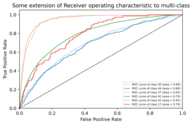
\includegraphics[width=1\linewidth]{bilder/ROC-Curve-Example.png}
		\caption{Multiple ROC-curves with different amount of thresholds each.}
		\label{plot:roc-multi}	
	\end{subfigure}%
	\hfill
	\begin{subfigure}[t]{0.49\hsize}\centering	
		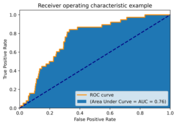
\includegraphics[width=1\linewidth]{bilder/ROC-Area-Example.png}
		\caption{\textbf{A}rea \textbf{U}nder \textbf{C}urve for The Receiver operating characteristic of a single class.}
		\label{plot:ROC-single}	
	\end{subfigure}
\end{figure}


The TP, FP, TN, FN counts then form the base for the following metrics (see equations \ref{metrics}):
\begin{figure}[H]
	\begin{equation} 
		\begin{aligned}
			\mathit{precision}_i &:= \frac{\mathit{TP_i}}{\mathit{TP_i}+\mathit{FP_i}} \\
			\mathit{recall}_i &:= \frac{\mathit{TP_i}}{\mathit{TP_i}+\mathit{FN_i}} \\
			\mathit{accuracy}_i &:= \frac{\mathit{TP_i}+\mathit{TN_i}}{\mathit{TP_i}+\mathit{TN_i}+\mathit{FP_i}+\mathit{FN_i}} \\
			\mathit{TPR}_i &:= \frac{\mathit{TP_i}}{\mathit{TP_i}+\mathit{FN_i}}\\
			\mathit{FPR}_i  &:= \frac{\mathit{FP_i}}{\mathit{FP_i}+\mathit{TN_i}}\\
			\mathit{F_{1,i}} &:= 2*\frac{\mathit{precision}_i*\mathit{recall}_i}{\mathit{precision}_i+\mathit{recall}_i}\\
			\mathit{ROC} \mathit{AUC}_i &:= \text{AUC of ROC-curve}\\%\\textbf{A}rea \textbf{U}nder the \textbf{C}urve of TPR plotted against FPR
		\end{aligned}
	\end{equation}
	\caption{Different score metrics to measure performance. All score functions calculate the score for a given class $i$.}
	\label{metrics}
\end{figure}

\begin{figure}[H]
	\begin{equation}
		\begin{aligned}
			\mathbf{macroavg}(\mathbf{score}) &:=\frac{1}{N}\sum_{i}^{N}\mathbf{score}(TP_i, FP_i, TN_i, FN_i)\\
			\mathbf{microavg}(\mathbf{score}) &:=\mathbf{score}(\mathit{TP}, \mathit{FP}, \mathit{TN}, \mathit{FN})\\
			&=\mathbf{score}(\sum \mathit{TP_i}, \sum \mathit{FP_i}, \sum \mathit{TN_i}, \sum \mathit{FN_i})\\
			\text{For example:}\\
			\mathbf{macroavg}(\mathit{TPR}) &:=\frac{1}{N}\sum_{i}^{N}\frac{\mathit{TP_i}}{\mathit{TP_i}+\mathit{FN_i}}\\
			\mathbf{microavg}(\mathit{TPR}) &:=\frac{\sum_{i}^{N}\mathit{TP_i}}{\sum_{i}^{N}\mathit{TP_i}+\sum_{i}^{N}\mathit{FN_i}}
		\end{aligned}
	\end{equation}
	%		\begin{equation}
	%			\begin{aligned}
	%				\mathit{precision} &:= \frac{\mathit{TP}}{\mathit{TP}+\mathit{FP}} \\
	%				\mathit{recall} &:= \frac{\mathit{TP}}{\mathit{TP}+\mathit{FN}} \\
	%				\mathit{accuracy} &:= \frac{\mathit{TP}+\mathit{TN}}{\mathit{TP}+\mathit{TN}+\mathit{FP}+\mathit{FN}} \\
	%				\mathit{TPR} &:= \frac{\mathit{TP}}{\mathit{TP}+\mathit{FN}}\\
	%				\mathit{FPR}  &:= \frac{\mathit{FP}}{\mathit{FP}+\mathit{TN}}\\
	%				\mathit{F_1} &:= 2*\frac{\mathit{precision}*\mathit{recall}}{\mathit{precision}+\mathit{recall}}\\
	%				\mathit{AUC} &:= \text{AUC of ROC-curve}\\%\\textbf{A}rea \textbf{U}nder the \textbf{C}urve \newline of TPR plotted against FPR
	%			\end{aligned}
	%		\end{equation}
	\caption{Micro- and Macro-average calculations for a given score function. Example for TPR at bottom}
	\label{metrics-avg}
\end{figure}

To obtain comparable results we also calculate \emph{micro}- and \emph{macro}-average scores (see equation \ref{metrics-avg}). The \emph{macro}-average sums the metrics in \autoref{metrics} for every individual class and averages by dividing through the number of classes. That way every class weighs the same in the resulting average, no matter how many samples that class has. The \emph{micro}-average can be calculated by summing the TPs, FPs, TNs and FNs for all classes respectively and then calculate the metrics in \autoref{metrics}, or by weighting the calculated class scores by their fraction of the total number of samples. The micro average thus weights the score metrics with the underlying class distribution. It is important to look at both micro and macro average scores to judge a models performance --- high micro average scores but low macro average scores suggest that small classes are being overlooked by the model, which is especially disastrous considering fatal illnesses are very rare in most cases. The opposite; a high macro average- but low micro average score suggests that the models accuracy in larger parts of the data is small, which, in our case, would most likely mean that healthy patients get diagnosed with illnesses on accident.

\subsubsection{Qualitative}
Apart from giving scores that allow a basic and quick evaluation of all of our models, we show various graphics for selected models to allow a more thorough overview of the models performance. They are explained in their respective section.

\section{Results}\label{sec:results}
\subsection{Quantitative}
\subsubsection{Baselines compared to CPC}

How does the CPC architecture compare against our baseline models in a fully supervised setting?

\begin{table}\centering
	\captionof{table}{Baseline Results}
	\resizebox{!}{0.2\textheight}{		
		\begin{adjustbox}{width=\textwidth}
\begin{tabular}{lrr}
{model} & {micro} & {macro} \\
BL\_alex\_v2 & 0.903 & 0.774 \\
BL\_FCN & 0.458 & 0.503 \\
BL\_MLP & 0.500 & 0.500 \\
BL\_TCN\_block & 0.876 & 0.638 \\
BL\_TCN\_down & 0.924 & 0.806 \\
BL\_TCN\_last & 0.869 & 0.649 \\
BL\_v0 & 0.916 & 0.787 \\
BL\_v0\_1 & 0.930 & 0.824 \\
BL\_v0\_2 & 0.867 & 0.664 \\
BL\_v0\_3 & 0.895 & 0.757 \\
BL\_v1 & 0.920 & 0.814 \\
BL\_v2 & 0.940 & 0.855 \\
BL\_v4 & 0.930 & 0.830 \\
BL\_v5 & 0.865 & 0.668 \\
BL\_v7 & 0.924 & 0.817 \\
BL\_v8 & 0.937 & 0.847 \\
BL\_v9 & 0.933 & 0.844 \\
BL\_v14 & \bfseries \underline{0.951} & \bfseries \underline{0.885} \\
BL\_v15 & 0.931 & 0.840 \\
\end{tabular}
\end{adjustbox}
	}
	\label{tbl:BL-all-class-new}
	\caption*{\small Micro and Macro AUC-ROC scores for all baseline models. Baseline Models are trained on the downstream task for 120 epochs.}
\end{table}
\autoref{tbl:BL-all-class-new} shows the results for our baseline/literature models. 
The literature architecture \code{BL\_v14}, which is tuned for timeseries classification by making use of parallel architectures with differently sized receptive fields, performs the best for both micro and macro ROC-AUC scores. This model performed the best compared to all models in general.

The fully connected network \code{BL\_FCN} and the multilayer perceptron \code{BL\_MLP} both failed to learn the data beyond random guessing classes. 

The best Temporal Convolutional Network is \code{BL\_TCN\_down} which uses a convolutional layer with filtersize $1$ to summarize the values in the data dimension. 

At this place we also want to mention the \code{BL\_v8} model which performed well and is used as encoder network in selected CPC models later on.

We compare the baseline network results to different CPC models (with the standard encoder-, context- and predictor-network), that were trained fully supervised for 120 epochs, to obtain their best possible scores within the 120 epoch limit. These results can be seen in \autoref{tbl:aucscores-cpc-nopretrain120}:
\begin{table}\centering
	\captionof{table}{CPC as Baseline Results}
	\resizebox{\textwidth}{!}{	
		\begin{adjustbox}{width=\textwidth}
\begin{tabular}{lrrlrr}
{model} & {Freeze CPC} & {strided} & {Downstream Model} & {micro} & {macro} \\
CPC & False & False & cpc\_downstream\_latent\_average & 0.943 & \bfseries \underline{0.879} \\
CPC & False & False & cpc\_downstream\_latent\_maximum & \bfseries \underline{0.944} & 0.877 \\
CPC & False & False & cpc\_downstream\_twolinear\_v2 & 0.933 & 0.845 \\
CPC & False & True & cpc\_downstream\_latent\_average & 0.941 & 0.872 \\
CPC & False & True & cpc\_downstream\_latent\_maximum & 0.941 & 0.873 \\
CPC & False & True & cpc\_downstream\_twolinear\_v2 & 0.924 & 0.831 \\
\end{tabular}
\end{adjustbox}
	}
	\caption*{\small CPC Models trained without pretraining for 120 epochs (with labels). All models shown use the standard encoder-, context-network}
	\label{tbl:aucscores-cpc-nopretrain120}
\end{table}
The models trained without pretraining have overall high average scores, only falling slightly behind \code{BL\_v14} (Multi-Scale-Residual Network), which proves the CPC architecture itself is clearly capable of classifying the data sufficiently in a supervised setting. 

The intersected models have a slim edge over strided models (\autoref{sec:cpc-strided}), most likely because they are less restrictive.

Surprisingly the models that utilized the more expressive two layer linear network fell slightly behind in performance, which we can only explain by a higher training difficulty, as the deeper model should be able to at least match the performance of smaller models. Similar occurrences have been already observed in the past, well explained in the Deep Residual Network paper \autocite{he2015deep}.

\subsubsection{CPC Downstream task with frozen weights}
How capable is CPC's pretraining? How good are the learned representations on their own? 

We want to measure how good the latent vector features are suited in our downstream task, by pretraining the model for 100 epochs without labels and downstream train for only 20 epochs with labels available. After pretraining, we are not updating any weights in the whole CPC network (CPC network is "frozen"). This is to say only the weights in the specific downstream task network (see \autoref{sec:cpc-downnetwork}) are altered during backpropagation. 
\begin{table}\centering
	\captionof{table}{CPC ROC-AUC scores, with no CPC layers updated during downstream training}
	\resizebox{\textwidth}{!}{
		\begin{adjustbox}{width=\textwidth}
\begin{tabular}{lrrllrr}
{model} & {Freeze CPC} & {strided} & {CPC Sampling Mode} & {Downstream Model} & {micro} & {macro} \\
CPC & True & False & all & cpc\_downstream\_latent\_average & 0.899 & 0.792 \\
CPC & True & False & all & cpc\_downstream\_latent\_maximum & 0.910 & 0.797 \\
CPC & True & False & all & cpc\_downstream\_twolinear\_v2 & 0.889 & 0.816 \\
CPC & True & False & crossentropy & cpc\_downstream\_latent\_average & 0.912 & 0.788 \\
CPC & True & False & crossentropy & cpc\_downstream\_latent\_maximum & 0.908 & 0.780 \\
CPC & True & False & crossentropy & cpc\_downstream\_twolinear\_v2 & 0.872 & 0.809 \\
CPC & True & False & same & cpc\_downstream\_latent\_average & 0.903 & 0.772 \\
CPC & True & False & same & cpc\_downstream\_latent\_maximum & 0.901 & 0.802 \\
CPC & True & False & same & cpc\_downstream\_twolinear\_v2 & 0.882 & \bfseries \underline{0.823} \\
CPC & True & True & all & cpc\_downstream\_latent\_average & 0.902 & 0.766 \\
CPC & True & True & all & cpc\_downstream\_latent\_maximum & 0.904 & 0.779 \\
CPC & True & True & all & cpc\_downstream\_twolinear\_v2 & 0.900 & 0.806 \\
CPC & True & True & crossentropy & cpc\_downstream\_latent\_average & 0.896 & 0.715 \\
CPC & True & True & crossentropy & cpc\_downstream\_latent\_maximum & 0.896 & 0.708 \\
CPC & True & True & crossentropy & cpc\_downstream\_twolinear\_v2 & 0.872 & 0.793 \\
CPC & True & True & same & cpc\_downstream\_latent\_average & 0.905 & 0.780 \\
CPC & True & True & same & cpc\_downstream\_latent\_maximum & 0.903 & 0.794 \\
CPC & True & True & same & cpc\_downstream\_twolinear\_v2 & \bfseries \underline{0.917} & 0.808 \\
\end{tabular}
\end{adjustbox}
	}
	\caption*{ ROC-AUC scores for standard CPC models trained with pretraining for 100 and training on the downstream task for 20 epochs (with the CPC weights frozen).} %TODO: say that crossentropy = all in subset
	\label{tbl:aucscores-cpc-pretrain-frozen}
\end{table}
The results in \autoref{tbl:aucscores-cpc-pretrain-frozen} show good results, however it is clear that they fall behind in performance compared to the models who had access to the labeled data for 120 epochs. We observe that the two layered linear network is the best performing downstream model, suggesting that the learned latent vectors are not fully linearly separable for this downstream task. The added complexity from introducing a second layer helped classifying the learned latent representations, in contrast to the networks trained purely on the downstream task, where the added complexity lead to lower scores.

Additionally the strided models show lower macro scores.

In comparison we show the results for the same models with randomly initialized weights and no pretraining whatsoever, as to prove the pretraining is actually relevant and the data is not just classifiable with random weights and a single/two layer(s) within 20 epochs of training time: \autoref{tbl:aucscores-cpc-nopretrain-frozen20}. 

As expected the models fail to satisfactorily classify the ecg-data, which becomes clear when looking at the macro ROC-AUC scores. The high micro scores suggest that one layer is still enough to learn the big parts of the data somehow, where one has to keep in mind that e.g. the biggest class "Sinus Rythm" is included in $\approx50\%$ of all ecg-files, which means correctly predicting this class has a big positive impact on micro average scores. (Reminder: see \autoref{fig:ClassCountsBar} for all classes.)
\begin{table}\centering
	\captionof{table}{CPC ROC-AUC scores, random weight initialization, no CPC layers updated during downstream training}
	\resizebox{\textwidth}{!}{
		\begin{adjustbox}{width=\textwidth}
\begin{tabular}{lrrlrr}
{model} & {Freeze CPC} & {strided} & {Downstream Model} & {micro} & {macro} \\
CPC & True & False & cpc\_downstream\_latent\_average & 0.852 & 0.514 \\
CPC & True & False & cpc\_downstream\_latent\_maximum & 0.861 & 0.580 \\
CPC & True & False & cpc\_downstream\_twolinear\_v2 & \bfseries \underline{0.864} & \bfseries \underline{0.582} \\
CPC & True & True & cpc\_downstream\_latent\_average & 0.853 & 0.510 \\
CPC & True & True & cpc\_downstream\_latent\_maximum & 0.852 & 0.575 \\
CPC & True & True & cpc\_downstream\_twolinear\_v2 & 0.861 & 0.577 \\
\end{tabular}
\end{adjustbox}
	}
	\caption{ROC-AUC scores for standard CPC models without pretraining (random weights); trained for 20 epochs on the downstream task (with the CPC weights frozen)}
	\label{tbl:aucscores-cpc-nopretrain-frozen20}
\end{table}
Both table \autoref{tbl:aucscores-cpc-pretrain-frozen} and \autoref{tbl:aucscores-cpc-nopretrain-frozen20} together suggest that the features learned by CPC in an unsupervised fashion are useful for the supervised downstream task, even if the network is restricted by making weight updates only in a previously untrained new layer, which fits the extracted features to the classes.

\subsubsection{CPC Downstream task with all weights updated}
Can the performance be improved by updating the weights in the whole architecture?

To answer this question, \autoref{tbl:aucscores-cpc-pretrain-unfrozen} shows yet another way of training the CPC architecture: pretrain the representations for 100 epochs and then, when training on the downstream task, do not freeze the weights in the CPC network layers. We assume, compared to the frozen model, this would lead to the better overall prediction accuracy, because the CPC pretraining is utilized in order to train the autoregressive architecture and then all weights are fine-tuned to optimize the classification loss.

As expected we observe that most models receive a slight performance boost compared to the "frozen" model variants and again the two layer downstream network has better scores overall. 
For the models however, that are trained with fewer latent vectors (\code{cpc\_intersect\_manylatents}) and use "crossentropy" non-strided, we observe that the complete opposite is the case: While the micro ROC-AUC scores are still in line with the other models, the macro average scores are worse than the models that did not have their weights updated. We assume the cpc objective lead to a specific latent representation that were in an opposite direction of the downstream loss function. With more training epochs, we assume that the model will converge towards the results of \autoref{tbl:aucscores-cpc-nopretrain120}, assuming the model can get out of the suboptimal local minimum. We cannot completely rule out overfitting, but we think it is unlikely in this case as the micro average scores are also lower than before.
%To explain the lower two linear layer performance in the models without pretrain we further argue that the added flexibility hurt Interestingly, comparing these results the same models that have been trained without  to no pretrain two layer < pooling. arguemtn source: difficulty to train latent representations if downstream too flexible in no pretrain.
\begin{table}\centering
	\captionof{table}{CPC ROC-AUC scores, with all layers updated in downstream training}
	\resizebox{\textwidth}{!}{
		\begin{adjustbox}{width=\textwidth}
\begin{tabular}{lrrllrr}
{model} & {Freeze CPC} & {strided} & {CPC Sampling Mode} & {Downstream Model} & {micro} & {macro} \\
CPC & False & False & all & cpc\_downstream\_latent\_average & 0.911 & 0.800 \\
CPC & False & False & all & cpc\_downstream\_latent\_maximum & 0.914 & 0.810 \\
CPC & False & False & all & cpc\_downstream\_twolinear\_v2 & 0.900 & 0.818 \\
CPC & False & False & crossentropy & cpc\_downstream\_latent\_average & 0.898 & 0.763 \\
CPC & False & False & crossentropy & cpc\_downstream\_latent\_maximum & 0.902 & 0.785 \\
CPC & False & False & crossentropy & cpc\_downstream\_twolinear\_v2 & 0.887 & 0.803 \\
CPC & False & False & same & cpc\_downstream\_latent\_average & 0.898 & 0.828 \\
CPC & False & False & same & cpc\_downstream\_latent\_maximum & 0.901 & 0.832 \\
CPC & False & False & same & cpc\_downstream\_twolinear\_v2 & 0.896 & \bfseries \underline{0.851} \\
CPC & False & True & all & cpc\_downstream\_latent\_average & 0.921 & 0.837 \\
CPC & False & True & all & cpc\_downstream\_latent\_maximum & 0.919 & 0.821 \\
CPC & False & True & all & cpc\_downstream\_twolinear\_v2 & \bfseries \underline{0.931} & 0.845 \\
CPC & False & True & crossentropy & cpc\_downstream\_latent\_average & 0.888 & 0.791 \\
CPC & False & True & crossentropy & cpc\_downstream\_latent\_maximum & 0.892 & 0.792 \\
CPC & False & True & crossentropy & cpc\_downstream\_twolinear\_v2 & 0.881 & 0.824 \\
CPC & False & True & same & cpc\_downstream\_latent\_average & 0.911 & 0.837 \\
CPC & False & True & same & cpc\_downstream\_latent\_maximum & 0.913 & 0.828 \\
CPC & False & True & same & cpc\_downstream\_twolinear\_v2 & 0.905 & 0.847 \\
\end{tabular}
\end{adjustbox}
	}
	\caption*{\small ROC-AUC scores for CPC models trained with pretraining for 100 epochs and training on the downstream task for 20 epochs with the CPC weights also updated.}
	\label{tbl:aucscores-cpc-pretrain-unfrozen}
\end{table}





\subsubsection{Low label availability}\label{section:lowlabel}
Under what circumstances is CPC especially efficient to use?

To further investigate the strengths of representation learning we reproduce an experiment from \autocite{cpcdataefficient} that omits labeled data in the training process to simulate data scarcity. Since the representations learned by CPC only rely on unlabeled data, a clear advantage for all CPC models compared to the baselines, which cannot make use of unlabeled data, can be expected. 

We start by utilizing the old train-, validation- and test-splits and make changes to the training split by taking a fixed fraction of each class. For this experiment, class label proportions of $\{0.7, 0.6, 0.5, 0.4, 0.3, 0.2, 0.1, 0.05, 0.01, 0.005, 0.001\}$ have been desired to achieve. Since the data can have multiple labels per sample, it is difficult or sometimes even impossible to exactly match the desired fractions for all classes, hence why the class distribution will be approximate. Our algorithm uses a greedy approach where all files are put into \enquote{class buckets} for each of the files corresponding class. Afterwards a random file is taken from each class bucket ordered by the buckets size, starting with the smallest one. If a file gets randomly drawn, it is removed from all other buckets. This gets repeated until all the desired fractions for each bucket are met. Code can be found in \code{experiment/create\_fewer\_labels\_data}.


Again, like in the other experiments, we train 120 epochs per baseline model, while CPC trains only for 20 epochs on the labeled data plus 100 epochs on ALL of the original training dataset without the labels.

Finally we measure micro and macro ROC-AUC scores on the same test dataset and plot the results. Instead of the desired proportion we use the actual fraction of total data files used as x-axis, because again, multiple classes are possible per sample, and the actual fraction of data used might differ from the desired proportions. The results for 20 epochs on cpc models and 120 epochs on baseline models can be seen in \autoref{plot:low-label}. As one can see more data $\equiv$ better score in general, however the CPC model scores are lower than in baseline models, where few labels are given. The lower CPC ROC-AUC score is contrary to what is to be expected since representation learning makes use of the complete dataset without labels first, hence it should perform considerably better in tasks that provide only few labeled data.
\begin{figure}
	\caption{Test scores for different models trained with a fraction of data labels} %TODO: make bigger maybe
	\begin{subfigure}[t]{0.99\textwidth}\centering
		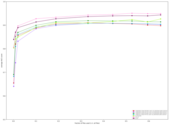
\includegraphics[width=1\linewidth]{bilder/2lowlabel-micro-20.png}%bilder/low_label_availability_classweightsmicro.png
		\caption{Micro average ROC-AUC score. Dashed Line: CPC models, Full Line: Baselines. Baseline-epochs: 120, CPC-epochs: 20}
		\label{fig:low-label-micro}	
	\end{subfigure}

	\begin{subfigure}[t]{0.99\textwidth}\centering
		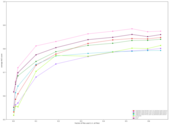
\includegraphics[width=1\linewidth]{bilder/2lowlabel-macro-20.png}%
		\caption{Macro Average ROC-AUC score. Dashed Line: CPC models, Full Line: Baselines. Baseline-epochs: 120, CPC-epochs: 20}
		\label{fig:low-label-macro}	
	\end{subfigure}
	\label{plot:low-label}
\end{figure}

To investigate this counter-intuitive behavior we train selected CPC models for 50 epochs instead of 20. We visualize the scores again in \autoref{plot:low-label-more} and this time see results closer to what we expected, where CPC models have a slight advantage over baseline models in very low label regimes. Interestingly the performance advantage quickly fades as more labels are given, no matter if trained for 20 or 50 epochs. Our hypothesis is that each class has to be shown to the model a specific number of times at least to successfully fit the model to the classification problem. By using less and less labels, while also limiting the CPC network to training for only 20 epochs, this hypothetical threshold, where the loss is not decreased enough for each individual class, must have been reached. We conclude that CPC is able to slightly outperform non-representation learning networks, where only very few labels are available, but needs sufficient epochs to do so. 

Nevertheless we are astounded how well the baselines performed in general and suspect that more tests on different data were few labels are available should be conducted in the future. 
\begin{figure}
	\caption{Test scores for different models trained with a fraction of data labels (more epochs)}
	\begin{subfigure}[t]{0.99\textwidth}\centering
		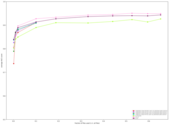
\includegraphics[width=1\linewidth]{bilder/2lowlabel-micro-50.png}%
		\caption{Micro average ROC-AUC score. Dashed Line: CPC models, Full Line: Baselines. Baseline-epochs: 120, CPC-epochs: 50}
		\label{fig:low-label-micro-more}	
	\end{subfigure}%
	\hfill	
	\begin{subfigure}[t]{0.99\textwidth}\centering
		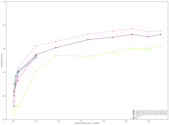
\includegraphics[width=1\linewidth]{bilder/2lowlabel-macro-50.png}%
		\caption{Macro Average ROC-AUC score. Dashed Line: CPC models, Full Line: Baselines. Baseline-epochs: 120, CPC-epochs: 50}
		\label{fig:low-label-macro-more}	
	\end{subfigure}
	\label{plot:low-label-more}
\end{figure}

Furthermore this experiment shows one of representation learnings biggest strength: time efficiency. While all the baseline models needed retraining for every single training dataset with 120 epochs each, totaling to more than 24 hours wall clock training time, the CPC model only needed the initial 100 epochs \textbf{that is shared amongst all datasets}, plus 20 (or 50) additional training epochs, greatly improving training time by a factor of almost 6 (or >2). Apart from low label availability this of course also the case for different downstream tasks, which is a great opportunity for saving power and time or for neural net enthusiasts that do not have access to capable hardware.

\subsubsection{Experiment: Training on Augmented Data} \label{sec:augmented}
Under what circumstances is CPC especially efficient to use?

We wanted to test whether CPC and the Baseline models are able to correctly predict classes with heavily augmented data, which might be useful for very noisy or even partially broken data. For this we applied the "min-max (augmented)" normalization function on the ecg data and trained the models after. \autoref{fig:ecg-augmented} shows the augmented data.
\begin{figure}[h]
	\caption{Normalized ECG example from beginning \autoref{fig:ECGBasic}}
	\begin{subfigure}[t]{0.48\textwidth}\centering
		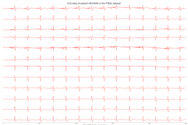
\includegraphics[width=1\linewidth]{bilder/ecg-example-minmax0.png}%
		\caption{Correct Min-Max Normalization}
	\end{subfigure}%
	\hfill	
	\begin{subfigure}[t]{0.48\textwidth}\centering
		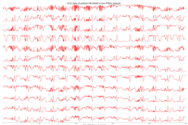
\includegraphics[width=1\linewidth]{bilder/ecg-example-augmented0.png}%
		\caption{Augmented Min-Max Normalization}
	\end{subfigure}
	\label{fig:ecg-augmented}
\end{figure}

The following tables show the results for training (and pretraining) multiple baseline and CPC-networks with different training settings on the augmented data. Note that for this section, we used slightly different downstream CPC networks compared to prior results (we refer to \autoref{cpc-architecture} for their description).

Table \ref{tbl:aucscores-avg-bl-class-stab} and table \ref{tbl:aucscores-avg-bl-noclass-stab} show the ROC-AUC scores for all the trained baseline models, while table \ref{tbl:aucscores-avg-cpc-class-stab} and table \ref{tbl:aucscores-avg-cpc-noclass-stab} show the AUC scores for all trained cpc models. The left shows the results with class weights utilized in the loss calculation, while the right shows all scores for the same models without the class weights. We make this differentiation, because the macro average scores, which are normally improved by factoring in the class weights during training, were heavily degraded by making use of this method. We suspect the different normalization made the training process more unstable and the added class-weights, which alter the loss directly, contribute to that already unstable training.
\begin{figure}[H]
	\captionof{table}{Baseline ROC-AUC scores}
	\begin{subfigure}[t]{0.49\hsize}\centering	
		\begin{adjustbox}{width=\textwidth}
\begin{tabular}{lrr}
\toprule
{} &  micro &  macro \\
\textbf{model                              } &        &        \\
\midrule
\textbf{BL\_v0\_1                 } &  0.579 &  0.485 \\
\textbf{BL\_v0\_2                 } &  0.618 &  0.490 \\
\textbf{BL\_v0\_3                 } &  0.546 &  0.490 \\
\textbf{BL\_v0                   } &  0.522 &  0.501 \\
\textbf{BL\_v1                   } &  0.658 &  0.482 \\
\textbf{BL\_v2                   } &  0.563 &  0.514 \\
\textbf{BL\_v3                   } &  0.547 &  0.492 \\
\textbf{BL\_v4                   } &  0.404 &  0.504 \\
\textbf{BL\_v5                   } &  0.396 &  0.521 \\
\textbf{BL\_v6                   } &  0.454 &  0.522 \\
\textbf{BL\_v7                   } &  0.870 &  0.730 \\
\textbf{BL\_v8                   } &  0.465 &  0.496 \\
\textbf{BL\_v9                   } &  0.439 &  0.511 \\
\textbf{BL\_v14                  } &  0.524 &  0.501 \\
\textbf{BL\_v15                  } &  \underline{0.894} &  \underline{0.806} \\
\textbf{baseline\_FCN            } &  0.484 &  0.505 \\
\textbf{baseline\_MLP            } &  0.500 &  0.500 \\
\textbf{baseline\_TCN\_block      } &  0.615 &  0.500 \\
\textbf{baseline\_TCN\_down       } &  0.874 &  0.747 \\
\textbf{baseline\_TCN\_flatten    } &  0.841 &  0.547 \\
\textbf{baseline\_TCN\_last       } &  0.846 &  0.567 \\
\textbf{baseline\_alex\_v2        } &  0.836 &  0.500 \\
\textbf{baseline\_rnn\_simplest\_lstm} &  0.834 &  0.532 \\
\bottomrule
\end{tabular}
\end{adjustbox}
		\caption{Models trained with class weights in the loss function.}
		\label{tbl:aucscores-avg-bl-class-stab}	
	\end{subfigure}%
	\vline
	\begin{subfigure}[t]{0.49\hsize}\centering
		\begin{adjustbox}{width=\textwidth}
\begin{tabular}{lrr}
\toprule
{} &  micro &  macro \\
\textbf{model                             } &        &        \\
\midrule
\textbf{BL\_v0\_1                   } &  0.835 &  0.773 \\
\textbf{BL\_v0\_2                   } &  0.856 &  0.680 \\
\textbf{BL\_v0\_3                   } &  0.854 &  0.676 \\
\textbf{BL\_v0                     } &  0.861 &  0.768 \\
\textbf{BL\_v1                     } &  \underline{0.917} &  0.800 \\
\textbf{BL\_v2                     } &  0.891 &  0.840 \\
\textbf{BL\_v3                     } &  0.852 &  0.813 \\
\textbf{BL\_v4                     } &  0.777 &  0.690 \\
\textbf{BL\_v5                     } &  0.866 &  0.640 \\
\textbf{BL\_v6                     } &  0.667 &  0.436 \\
\textbf{BL\_v7                     } &  0.838 &  0.533 \\
\textbf{BL\_v8                     } &  0.891 &  \underline{0.842} \\
\textbf{BL\_v9                     } &  0.875 &  0.839 \\
\textbf{BL\_v14                    } &  0.886 &  0.841 \\
\textbf{BL\_v15                    } &  0.884 &  0.813 \\
\textbf{baseline\_FCN              } &  0.607 &  0.502 \\
\textbf{baseline\_MLP              } &  0.500 &  0.500 \\
\textbf{baseline\_TCN\_block        } &  0.628 &  0.500 \\
\textbf{baseline\_TCN\_down         } &  0.785 &  0.727 \\
\textbf{baseline\_TCN\_flatten      } &  0.855 &  0.584 \\
\textbf{baseline\_TCN\_last                 } &  0.857 &  0.576 \\
\textbf{baseline\_alex\_v2          } &  0.851 &  0.500 \\
\textbf{baseline\_rnn\_simplest\_lstm} &  0.848 &  0.585 \\
\bottomrule
\end{tabular}
\end{adjustbox}
		\caption{Models trained without class weights in the loss function.}
		\label{tbl:aucscores-avg-bl-noclass-stab}	
	\end{subfigure}
	\label{tbl:aucscores-avg-bl-stab}
\end{figure}
\begin{figure}[H]
	\captionof{table}{CPC ROC-AUC scores} %TODO: use new table layout (produce plots)
	\begin{subfigure}[t]{0.49\hsize}\centering	
		\begin{adjustbox}{width=\textwidth}
\begin{tabular}{lrr}
\toprule
{} &  micro &  macro \\
\textbf{model                                               } &        &        \\
\midrule
\textbf{CPC|frozen|C|L|m:all|cnn               } &  0.888 &  0.825 \\
\textbf{CPC|frozen|C|L|m:all|twolinear         } &  0.889 &  0.822 \\
\textbf{CPC|frozen|C|L|m:same|cnn              } &  0.904 &  0.849 \\
\textbf{CPC|frozen|C|L|m:same|twolinear        } &  0.885 &  0.810 \\
\textbf{CPC|frozen|C|m:all|cnn                   } &  0.890 &  0.813 \\
\textbf{CPC|frozen|C|m:all|linear              } &  0.914 &  0.810 \\
\textbf{CPC|frozen|C|m:all|twolinear             } &  0.875 &  0.783 \\
\textbf{CPC|frozen|C|m:same|cnn                  } &  0.918 &  0.822 \\
\textbf{CPC|frozen|C|m:same|linear             } &  0.918 &  0.834 \\
\textbf{CPC|frozen|C|m:same|twolinear            } &  0.900 &  0.839 \\
\textbf{CPC|frozen|L|m:all|cnn                   } &  0.883 &  0.832 \\
\textbf{CPC|frozen|L|m:all|linear              } &  0.910 &  0.844 \\
\textbf{CPC|frozen|L|m:all|twolinear             } &  0.897 &  0.825 \\
\textbf{CPC|frozen|L|m:same|cnn                  } &  0.914 &  0.769 \\
\textbf{CPC|frozen|L|m:same|linear             } &  0.841 &  0.708 \\
\textbf{CPC|frozen|L|m:same|twolinear            } &  0.903 &  0.779 \\
\textbf{CPC|strided|frozen|C|L|m:all|cnn       } &  0.909 &  0.780 \\
\textbf{CPC|strided|frozen|C|L|m:all|twolinear } &  0.776 &  0.545 \\
\textbf{CPC|strided|frozen|C|L|m:same|cnn      } &  0.895 &  0.771 \\
\textbf{CPC|strided|frozen|C|L|m:same|twolinear} &  0.751 &  0.591 \\
\textbf{CPC|strided|frozen|C|m:all|cnn           } &  \underline{0.921} &  0.792 \\
\textbf{CPC|strided|frozen|C|m:all|linear      } &  \underline{0.921} &  0.812 \\
\textbf{CPC|strided|frozen|C|m:all|twolinear     } &  0.911 &  0.795 \\
\textbf{CPC|strided|frozen|C|m:same|cnn          } &  0.903 &  0.754 \\
\textbf{CPC|strided|frozen|C|m:same|linear     } &  0.892 &  0.841 \\
\textbf{CPC|strided|frozen|C|m:same|twolinear    } &  0.898 &  0.833 \\
\textbf{CPC|strided|frozen|L|m:all|cnn           } &  0.898 &  0.836 \\
\textbf{CPC|strided|frozen|L|m:all|linear      } &  0.884 &  0.806 \\
\textbf{CPC|strided|frozen|L|m:all|twolinear     } &  0.898 &  0.838 \\
\textbf{CPC|strided|frozen|L|m:same|cnn          } &  0.876 &  0.824 \\
\textbf{CPC|strided|frozen|L|m:same|linear     } &  0.910 &  \underline{0.852} \\
\textbf{CPC|strided|frozen|L|m:same|twolinear    } &  0.885 &  0.844 \\
\bottomrule
\end{tabular}
\end{adjustbox}
		\caption{Models trained with class weights in the loss function.}
		\label{tbl:aucscores-avg-cpc-class-stab}
	\end{subfigure}
	\vline
	\begin{subfigure}[t]{0.49\hsize}\centering %\captionof{table}{CPC AUC scores without class\_weights}	
		\begin{adjustbox}{width=\textwidth}
\begin{tabular}{lrr}
\toprule
{} &  micro &  macro \\
\textbf{model                                               } &        &        \\
\midrule
\textbf{CPC|frozen|C|L|m:all|cnn               } &  0.901 &  0.829 \\
\textbf{CPC|frozen|C|L|m:all|twolinear         } &  0.838 &  0.808 \\
\textbf{CPC|frozen|C|L|m:same|cnn              } &  0.886 &  \underline{0.843} \\
\textbf{CPC|frozen|C|L|m:same|twolinear        } &  0.877 &  \underline{0.843} \\
\textbf{CPC|frozen|C|m:all|cnn                 } &  0.914 &  0.766 \\
\textbf{CPC|frozen|C|m:all|linear            } &  \underline{0.921} &  0.812 \\
\textbf{CPC|frozen|C|m:all|twolinear           } &  0.902 &  0.834 \\
\textbf{CPC|frozen|C|m:same|cnn                } &  0.916 &  0.791 \\
\textbf{CPC|frozen|C|m:same|linear           } &  0.911 &  0.795 \\
\textbf{CPC|frozen|C|m:same|twolinear          } &  0.882 &  \underline{0.843} \\
\textbf{CPC|frozen|L|m:all|cnn                 } &  0.842 &  0.775 \\
\textbf{CPC|frozen|L|m:all|linear            } &  0.769 &  0.540 \\
\textbf{CPC|frozen|L|m:all|twolinear           } &  0.834 &  0.785 \\
\textbf{CPC|frozen|L|m:same|cnn                } &  0.862 &  0.802 \\
\textbf{CPC|frozen|L|m:same|linear           } &  0.781 &  0.595 \\
\textbf{CPC|frozen|L|m:same|twolinear          } &  0.860 &  0.814 \\
\textbf{CPC|strided|frozen|C|L|m:all|cnn       } &  0.867 &  0.823 \\
\textbf{CPC|strided|frozen|C|L|m:all|twolinear } &  0.865 &  0.817 \\
\textbf{CPC|strided|frozen|C|L|m:same|cnn      } &  0.565 &  0.549 \\
\textbf{CPC|strided|frozen|C|L|m:same|twolinear} &  0.870 &  0.814 \\
\textbf{CPC|strided|frozen|C|m:all|cnn         } &  0.917 &  0.822 \\
\textbf{CPC|strided|frozen|C|m:all|linear    } &  \underline{0.921} &  0.792 \\
\textbf{CPC|strided|frozen|C|m:all|twolinear   } &  0.914 &  0.842 \\
\textbf{CPC|strided|frozen|C|m:same|cnn        } &  0.917 &  0.828 \\
\textbf{CPC|strided|frozen|C|m:same|linear   } &  0.909 &  0.779 \\
\textbf{CPC|strided|frozen|C|m:same|twolinear  } &  0.897 &  0.838 \\
\textbf{CPC|strided|frozen|L|m:all|cnn         } &  0.858 &  0.799 \\
\textbf{CPC|strided|frozen|L|m:all|linear    } &  0.902 &  0.775 \\
\textbf{CPC|strided|frozen|L|m:all|twolinear   } &  0.822 &  0.795 \\
\textbf{CPC|strided|frozen|L|m:same|cnn        } &  0.848 &  0.799 \\
\textbf{CPC|strided|frozen|L|m:same|linear   } &  0.895 &  0.781 \\
\textbf{CPC|strided|frozen|L|m:same|twolinear  } &  0.828 &  0.794 \\
\bottomrule
\end{tabular}
\end{adjustbox}
		\caption{Models trained without class weights in the loss function.}
		\label{tbl:aucscores-avg-cpc-noclass-stab}	
	\end{subfigure}	
	\caption*{\small Legend:\newline
		\hl{m:all} All latents are used as negative examples in the cpc loss.
		\hl{m:same} Latents only from the same timestep are used as negative examples.
		\hl{linear/cnn/twolinear/latent\_maximum} The used downstream architecture.
		\hl{L} Latent vectors are used for predicting the class labels.
		\hl{C} Context vector is used for predicting the class labels.
		\hl{frozen} The weights are not updated in the cpc network layers during downstream task.
		\hl{strided} Disjoint window data encoder is used instead.}
	\label{tbl:aucscores-avg-cpc-stab}
\end{figure}
%(TODO: maybe insert scatter plot? What is X?)
We see that CPC overall performs the best in terms of ROC-AUC score, although labels have not been used as often as in the baseline models. Interesting to see is also that the baseline models cannot cope well with the class weights added to the loss function: Most models cannot confidently surpass even an ROC-AUC area of 0.5, which is the threshold for random guessing. However we admit that the performance drop for the baseline models with the class weights added is suspiciously high and might suggest other factors such as non ideal training settings, that affect weighted models only, are the root of this problem. 

Having said this, all CPC models, with only few exceptions, do not see this degradation in performance, meaning they fit all classes in the augmented dataset. As a result we observe better macro average values in some cases with the weights added to the loss function.
The overall badly performing baselines and the few CPC models that completely fail to classify the augmented data, suggest that the training for this task is extremely unstable.

To determine whether this difference in performance is caused by the pretraining step or the architecture itself we additionally train a few new CPC models fully supervised without the pretraining step for 120 epochs. 
\begin{figure}
	\captionof{table}{Average CPC ROC-AUC scores, no pretraining}
	\begin{subfigure}[t]{0.49\hsize}\centering
		\begin{adjustbox}{width=\textwidth}
\begin{tabular}{lrr}
\toprule
{} &  micro &  macro \\
\textbf{model                                            } &        &        \\
\midrule
\textbf{CPC|strided|unfrozen|C|m:all|cnn   } &  \underline{0.889} &  \underline{0.864} \\
\textbf{CPC|strided|unfrozen|C|m:all|linear} &  0.808 &  0.482 \\
\textbf{CPC|strided|unfrozen|L|m:all|cnn   } &  0.868 &  0.825 \\
\textbf{CPC|strided|unfrozen|L|m:all|linear} &  0.874 &  0.815 \\
\textbf{CPC|unfrozen|C|m:all|cnn           } &  0.828 &  0.598 \\
\textbf{CPC|unfrozen|C|m:all|linear        } &  0.788 &  0.642 \\
\textbf{CPC|unfrozen|L|m:all|cnn           } &  0.824 &  0.499 \\
\textbf{CPC|unfrozen|L|m:all|linear        } &  0.772 &  0.536 \\
\bottomrule
\end{tabular}
\end{adjustbox}
		\caption{No class weights were used in loss function.}
		\label{tbl:aucscores-cpcno-pretrain-noclass-stab}
	\end{subfigure}
	\begin{subfigure}[t]{0.49\hsize}\centering
		\begin{adjustbox}{width=\textwidth}
\begin{tabular}{lrr}
\toprule
{} &  micro &  macro \\
\textbf{model                                             } &        &        \\
\midrule
\textbf{CPC|strided|unfrozen|C|m:all|cnn   } &  \underline{0.918} &  \underline{0.833} \\
\textbf{CPC|strided|unfrozen|C|m:all|linear} &  0.802 &  0.498 \\
\textbf{CPC|strided|unfrozen|L|m:all|cnn   } &  0.904 &  0.824 \\
\textbf{CPC|strided|unfrozen|L|m:all|linear} &  0.901 &  0.798 \\
\textbf{CPC|unfrozen|C|m:all|cnn           } &  0.820 &  0.498 \\
\textbf{CPC|unfrozen|C|m:all|linear        } &  0.803 &  0.497 \\
\textbf{CPC|unfrozen|L|m:all|cnn           } &  0.820 &  0.500 \\
\textbf{CPC|unfrozen|L|m:all|linear        } &  0.708 &  0.570 \\
\bottomrule
\end{tabular}
\end{adjustbox}
		\caption{Class weights were used in loss function.}
		\label{tbl:aucscores-cpcno-pretrain-class-stab}
	\end{subfigure}
	\caption*{\small ROC-AUC scores for CPC models trained without pretraining, trained on the downstream task for 120 epochs. Legend: (like in \autoref{tbl:aucscores-avg-cpc-class-stab})}
	\label{tbl:aucscores-cpcno-pretrain-stab}
\end{figure}
Comparing \autoref{tbl:aucscores-cpcno-pretrain-stab} to \autoref{tbl:aucscores-avg-cpc-stab}, the non-strided version of the model that used the context, did not work as good as the same model that was pretrained with the CPC-loss, especially the macro average degraded substantially. These results are in line with the baseline results in the stability experiment already observed. We argue that with heavily augmented/noised data, the CPC pretraining step is crucial to correctly learn the latent representations in the CPC architecture.

Interestingly, the \enquote{strided} CPC models do not exhibit such a big performance gap compared to the pretrained models and work well for both micro- and macro-average scores. We hypothesize that, even without pretraining, the \enquote{strided} architecture is easier to train due to fewer latent vectors being calculated, making it easier for downstream task networks.

Table \ref{tbl:aucscores-cpc-pretrain-unfrozen-noclassweights-stab} and Table \ref{tbl:aucscores-cpc-pretrain-unfrozen-classweights-stab} show yet another way of training the CPC architecture: pretrain the representations for 100 epochs and then, when training on the downstream task, do not freeze the weights in the CPC network layers:
\begin{figure}[H]
	\captionof{table}{CPC ROC-AUC scores, with all layers updated in downstream training}
	\begin{subfigure}[t]{0.48\textwidth}
		\begin{adjustbox}{width=\textwidth}
\begin{tabular}{lrr}
\toprule
{} &  micro &  macro \\
\textbf{model                                        } &        &        \\
\midrule
\textbf{CPC|strided|unfrozen|C|m:all|cnn} &  \underline{0.826} &  \underline{0.789} \\
\textbf{CPC|strided|unfrozen|L|m:all|cnn} &  0.818 &  0.752 \\
\textbf{CPC|unfrozen|C|m:all|cnn        } &  0.818 &  0.731 \\
\textbf{CPC|unfrozen|L|m:all|cnn        } &  0.819 &  0.499 \\
\bottomrule
\end{tabular}
\end{adjustbox}
		\caption{No class-weights are used.}
		\label{tbl:aucscores-cpc-pretrain-unfrozen-noclassweights-stab}
	\end{subfigure}
	\vline
	\begin{subfigure}[t]{0.48\textwidth}
		\begin{adjustbox}{width=\textwidth}
\begin{tabular}{lrr}
\toprule
{} &  micro &  macro \\
\textbf{model                                         } &        &        \\
\midrule
\textbf{CPC|strided|unfrozen|C|m:all|cnn} &  \underline{0.822} &  0.498 \\
\textbf{CPC|strided|unfrozen|L|m:all|cnn} &  0.821 &  0.498 \\
\textbf{CPC|unfrozen|C|m:all|cnn        } &  0.820 &  0.476 \\
\textbf{CPC|unfrozen|L|m:all|cnn        } &  0.821 &  \underline{0.520} \\
\bottomrule
\end{tabular}
\end{adjustbox}
		\caption{Class-weights are used.}
		\label{tbl:aucscores-cpc-pretrain-unfrozen-classweights-stab}
	\end{subfigure}
	\caption*{\small ROC-AUC scores for CPC models trained with pretraining for 100 epochs and training on the downstream task for 20 epochs with the CPC weights also updated.  Legend: (like in \autoref{tbl:aucscores-avg-cpc-class-stab})}
	\label{tbl:aucscores-cpc-pretrain-unfrozen-stab}
\end{figure}
At first one would assume this would lead to the best overall prediction accuracy, because the CPC pretraining is utilized in order to train the autoregressive architecture and then all weights are fine-tuned to optimize the classification loss. Yet we observe the opposite: while the micro-average ROC-AUC scores are still in line with the other models, the macro-average scores are the overall worst, at least in the training with added class weights. We assume the cpc objective lead to a specific latent representation that were in an opposite direction of the downstream loss function and acted like a bad weight initialization. With more training epochs, we assume that the model will converge towards the results of \autoref{tbl:aucscores-cpcno-pretrain-class-stab}, assuming the model can get out of the suboptimal local minimum. A different explanation is that the added flexibility allowed the model to more easily overfit on the training data.

Although the CPC models outperformed all baseline architectures (\autoref{tbl:aucscores-avg-bl-stab} vs. \autoref{tbl:aucscores-avg-cpc-stab}), which suggests that the pretraining step seems to help train the models, we cannot confidently say that pretraining is always helpful for augmented data because the strided CPC networks still perform well in a setting with no pretraining at all (see \autoref{tbl:aucscores-cpcno-pretrain-stab}), while some CPC models could not be succesfully trained even with pretraining. Since strided and non-strided models only vary in architecture and not how they are trained, it is possible that difference in the architecture lead to good performance and not the pretraining per se. Nevertheless we suspect that the CPC pretraining leads more easily to overall good representations if the data is difficult to classify, and that too much freedom during the difficult downstream task leads to overfitting or unstable training, which can be followed from \autoref{tbl:aucscores-avg-cpc-stab} vs. \autoref{tbl:aucscores-cpc-pretrain-unfrozen-stab}. We suspect the strided models get around overfitting because of easier model convergence. In summary we argue that the stability experiment results are inconclusive but they hint at that CPC models and their pretraining make finding the latent features easier, in unstable training environments.


\subsubsection{Additional changes}\label{sec:additionalchanges}
Can the original architecture be improved?

Next we take a look at the additional changes we made to the CPC architecture to allow a more flexible use or increase performance. In some cases we relaxed our downstream epoch limit from 20 to 40, because we are not directly compare to baseline networks and in order to more thoroughly test an architectures capabilities. We note that this increases the difficulty of comparing those models to the ones that only trained for 20 epochs above, but if the performance is still lower when trained for 40 epochs, we are more certain that this specific change in the architecture was a step in the wrong direction.

Additionally please note that for certain categories like "Downstream Model", we will only display the models with the highest macro average scores. For example a model that has been trained with \code{cpc\_downstream\_latent\_average} vs \code{cpc\_downstream\_latent\_maximum} with otherwise equal settings, will only show the better model with the associated scores. Also all models use \code{cpc\_intersect\_manylatents} (see \autoref{sec:fewerlatentvectors}) and --- besides their one changed module --- still the standard encoder-, context- and predictor network \code{cpc\_encoder\_v0}, \code{cpc\_autoregressive\_v0} and \code{cpc\_predictor\_v0}. This restriction is necessary since some models require to be trained with \code{cpc\_intersect\_manylatents} in order to function.

\autoref{tbl:aucscores-cpc-cross40} can be used as a reference for what is possible using all standard modules with 40 epochs (with \code{cpc\_intersect\_manylatents}).
\begin{table}\centering
	\captionof{table}{CPC ROC-AUC scores, 40 Downstream Epochs}
	\resizebox{\textwidth}{!}{
		\begin{adjustbox}{width=\textwidth}
\begin{tabular}{lrrlrlrr}
{model} & {Freeze CPC} & {strided} & {CPC Sampling Mode} & {Downstream Epochs} & {Downstream Model} & {micro} & {macro} \\
CPC & False & False & crossentropy & 40.000 & cpc\_downstream\_latent\_average & \bfseries \underline{0.930} & \bfseries \underline{0.842} \\
CPC & False & False & crossentropy & 40.000 & cpc\_downstream\_latent\_maximum & 0.925 & 0.830 \\
CPC & False & False & crossentropy & 40.000 & cpc\_downstream\_twolinear\_v2 & 0.911 & 0.830 \\
CPC & False & True & crossentropy & 40.000 & cpc\_downstream\_latent\_average & 0.905 & 0.768 \\
CPC & False & True & crossentropy & 40.000 & cpc\_downstream\_latent\_maximum & 0.878 & 0.802 \\
CPC & False & True & crossentropy & 40.000 & cpc\_downstream\_twolinear\_v2 & 0.915 & 0.801 \\
CPC & True & False & crossentropy & 40.000 & cpc\_downstream\_latent\_average & 0.923 & 0.824 \\
CPC & True & False & crossentropy & 40.000 & cpc\_downstream\_latent\_maximum & 0.926 & 0.827 \\
CPC & True & False & crossentropy & 40.000 & cpc\_downstream\_twolinear\_v2 & 0.929 & 0.838 \\
CPC & True & True & crossentropy & 40.000 & cpc\_downstream\_latent\_average & 0.908 & 0.772 \\
CPC & True & True & crossentropy & 40.000 & cpc\_downstream\_latent\_maximum & 0.915 & 0.804 \\
CPC & True & True & crossentropy & 40.000 & cpc\_downstream\_twolinear\_v2 & 0.917 & 0.801 \\
\end{tabular}
\end{adjustbox}
	}
	\caption*{\small ROC-AUC scores for CPC models trained with pretraining for 100 epochs and training on the downstream task for 40 epochs.}
	\label{tbl:aucscores-cpc-cross40}
\end{table}

\paragraph{Normalized Latent Vectors}
\autoref{tbl:aucscores-cpc-normalized} shows the results for models that were trained with normalized latent vectors (see \autoref{sec:normalizedlatents} for details). We see that even with more epochs the scores are overall lower, for both micro and macro average, indicating this change most likely is not beneficial. We suspect that normalizing the vectors restricted the model too much.
\begin{table}\centering
	\captionof{table}{CPC ROC-AUC scores: normalized latents}
	\resizebox{\textwidth}{!}{
		\begin{adjustbox}{width=\textwidth}
\begin{tabular}{lrrrlrlrr}
{model} & {Freeze CPC} & {strided} & {normalizes latents} & {CPC Sampling Mode} & {Downstream Epochs} & {Downstream Model} & {micro} & {macro} \\
CPC & False & False & True & crossentropy & 20.000 & cpc\_downstream\_twolinear\_v2 & 0.873 & 0.659 \\
CPC & False & False & True & crossentropy & 40.000 & cpc\_downstream\_latent\_average & 0.905 & 0.774 \\
CPC & False & True & True & crossentropy & 20.000 & cpc\_downstream\_twolinear\_v2 & 0.869 & 0.750 \\
CPC & False & True & True & crossentropy & 40.000 & cpc\_downstream\_latent\_maximum & \bfseries \underline{0.916} & \bfseries \underline{0.799} \\
CPC & True & False & True & crossentropy & 20.000 & cpc\_downstream\_twolinear\_v2 & 0.845 & 0.690 \\
CPC & True & False & True & crossentropy & 40.000 & cpc\_downstream\_twolinear\_v2 & 0.887 & 0.697 \\
CPC & True & True & True & crossentropy & 20.000 & cpc\_downstream\_twolinear\_v2 & 0.879 & 0.754 \\
CPC & True & True & True & crossentropy & 40.000 & cpc\_downstream\_twolinear\_v2 & 0.902 & 0.753 \\
\end{tabular}
\end{adjustbox}
	}
	\caption*{\small ROC-AUC scores for CPC models trained with pretraining for 100 epochs and training on the downstream task for 20 or 40 epochs (both frozen/updated). Latent vectors are always normalized}
	\label{tbl:aucscores-cpc-normalized}
\end{table}

\paragraph{Encoder like Baseline\_v8}
In \autoref{tbl:aucscores-cpc-likev8} we see the results for models that were trained with \code{cpc\_encoder\_likev8}, which is a clone of the baseline model \code{BL\_v8}. \code{cpc\_encoder\_likev8} outputs 147 latent vectors as opposed to 26 like the standard architecture. We report lower scores overall.

Nevertheless we want to mention that generating more latent vectors is a trait which is useful in some tasks, as for example later on in \autoref{sec:explainingclasses}.
\begin{table}\centering
	\captionof{table}{CPC ROC-AUC scores: \code{cpc\_encoder\_likev8}}
	\resizebox{\textwidth}{!}{
		\begin{adjustbox}{width=\textwidth}
\begin{tabular}{lrrllrlrr}
{model} & {Freeze CPC} & {strided} & {CPC Sampling Mode} & {Encoder} & {Downstream Epochs} & {Downstream Model} & {micro} & {macro} \\
CPC & False & False & crossentropy & cpc\_encoder\_likev8 & 20.000 & cpc\_downstream\_twolinear\_v2 & 0.853 & 0.771 \\
CPC & True & False & crossentropy & cpc\_encoder\_likev8 & 20.000 & cpc\_downstream\_twolinear\_v2 & \bfseries \underline{0.873} & \bfseries \underline{0.787} \\
\end{tabular}
\end{adjustbox}
	}
	\caption*{\small ROC-AUC scores for CPC models trained with pretraining for 100 epochs and training on the downstream task for 20 or 40 epochs (both frozen/updated). \code{cpc\_encoder\_likev8} is always used as an encoder}
	\label{tbl:aucscores-cpc-likev8}
\end{table}

\paragraph{Hidden State Context Network}
We look at the results of our networks where \code{cpc\_autoregressive\_hidden} is used, which uses the hidden state as a context for the next step latent predictions. The model that was trained for 40 epochs with all weights updated yielded the best results, even surpassing the macro-average score from the best model in the comparison \autoref{tbl:aucscores-cpc-cross40}. Interestingly the score got degraded for the model with the weights frozen, making this context network useful only situational.
\begin{table}\centering
	\captionof{table}{CPC ROC-AUC scores: \code{cpc\_autoregressive\_hidden}}
	\resizebox{\textwidth}{!}{
		\begin{adjustbox}{width=\textwidth}
\begin{tabular}{lrrllrlrr}
{model} & {Freeze CPC} & {strided} & {CPC Sampling Mode} & {Autoregressive} & {Downstream Epochs} & {Downstream Model} & {micro} & {macro} \\
CPC & False & False & crossentropy & cpc\_autoregressive\_hidden & 40.000 & cpc\_downstream\_latent\_maximum & \bfseries \underline{0.927} & \bfseries \underline{0.851} \\
CPC & True & False & crossentropy & cpc\_autoregressive\_hidden & 40.000 & cpc\_downstream\_twolinear\_v2 & 0.885 & 0.797 \\
\end{tabular}
\end{adjustbox}
	}
	\caption*{\small ROC-AUC scores for CPC models trained with pretraining for 100 epochs and training on the downstream task for 20 or 40 epochs (both frozen/updated). \code{cpc\_autoregressive\_hidden} is always used as context network}
	\label{tbl:aucscores-cpc-hidden}
\end{table}

\paragraph{No Context Network}
For the network that did not use the context for predicting future latents, and instead a TCN trained to predict next-step latents directly, the results are overall a bit lower. Despite not displayed here, we mention that the CPC accuracy during pretraining was higher than for any other model, with exemption of models trained with the 'same' sampling method and all standard settings, indicating that the respresentations were more easily distinguishable for the different entries in the batch.
\begin{table}[h]\centering
	\captionof{table}{CPC ROC-AUC scores: \code{cpc\_predictor\_nocontext}}
	\resizebox{\textwidth}{!}{
		\begin{adjustbox}{width=\textwidth}
\begin{tabular}{lrrllrlrr}
{model} & {Freeze CPC} & {strided} & {CPC Sampling Mode} & {Predictor} & {Downstream Epochs} & {Downstream Model} & {micro} & {macro} \\
CPC & False & False & crossentropy-nocontext & cpc\_predictor\_nocontext & 20.000 & cpc\_downstream\_twolinear\_v2 & 0.873 & 0.762 \\
CPC & False & False & crossentropy-nocontext & cpc\_predictor\_nocontext & 40.000 & cpc\_downstream\_latent\_maximum & \bfseries \underline{0.913} & \bfseries \underline{0.831} \\
CPC & True & False & crossentropy-nocontext & cpc\_predictor\_nocontext & 20.000 & cpc\_downstream\_twolinear\_v2 & 0.881 & 0.764 \\
CPC & True & False & crossentropy-nocontext & cpc\_predictor\_nocontext & 40.000 & cpc\_downstream\_twolinear\_v2 & 0.911 & 0.803 \\
\end{tabular}
\end{adjustbox}
	}
	\caption*{\small ROC-AUC scores for CPC models trained with pretraining for 100 epochs and training on the downstream task for 20 or 40 epochs (both frozen/updated). \code{cpc\_predictor\_nocontext} is always used as the latent predictor}
	\label{tbl:aucscores-cpc-nocontext}
\end{table}
Although the results were slightly less accurate, we note that it is still interesting to see that the context network + single linear layers for predicting future latents is not a given and can be exchanged for different architectures.

\subsection{Qualitative}
\subsubsection{Finding the best Hyperparameters with Parallel Coordinates}
What are the best settings/hyperparameters for CPC?

To better evaluate what model specific baseline hyperparameters lead to a good test performance we make use of a so called \enquote{Parallel Coordinates} plot which can visualize high-dimensional datasets. It consists of one x-axis that uses a categorical label instead of a number at each step with no specific order and multiple differently ranged y-axes, one for each categorical label. Every datasample is drawn as line in a color specific to one of the datasamples attributes. In short, parallel coordinate plots visualize tables by using the column-headers as x-axis and draw each row as a line with a color specific to one selected column.

Since we want to figure out what hyper parameters influence our micro and macro ROC-AUC score in a positive way, both will be used individually as color in the plot, while some of the hyperparameters will be shown on the x-axis. We summarize list-like hyperparameters such as multiple strides or kernel-sizes as a sum in order to visualize them. For strides especially, a product could be used instead to deliver more accurate results, which is due to the fact that strides have a multiplcative impact on input data, while kernel-sizes are closer to additive. The widely different values however made the plot unreadable with big products in our case. The resulting plot can be seen in \autoref{fig:bl-parcoords-micro} and \autoref{fig:bl-parcoords-macro}. While it is difficult to judge most hyperparamters with confidence based on this plot, we can see that the final layer choice seems to have a big impact on performance in our baseline models. There, approach \ref{desc:en4} --- which downsamples the models output with a convolutional layer before feeding it to the final linear layer --- seems to achieve the overall best performance.
\begin{figure}[H]
	\caption{Parallel Coordinates Plot for all trained baseline networks from \autoref{tbl:aucscores-avg-bl-class-stab}.}
	\begin{subfigure}[t]{0.95\textwidth}\centering
		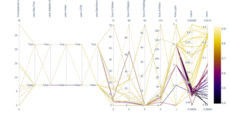
\includegraphics[width=1\linewidth]{bilder/bl-attributes-parallelcoordsmicro.png}
		\caption{The color is the \textbf{micro} ROC-AUC score}
		\label{fig:bl-parcoords-micro}	
	\end{subfigure}%
	
	\begin{subfigure}[t]{0.95\textwidth}\centering
		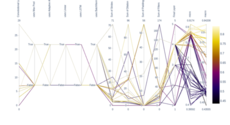
\includegraphics[width=1\linewidth]{bilder/bl-attributes-parallelcoordsmacro.png}
		\caption{The color is the \textbf{macro} ROC-AUC score}
		\label{fig:bl-parcoords-macro}	
	\end{subfigure}
\end{figure}

For the trained CPC models we use a different implementation obtained from Github\footcite{https://github.com/jraine/parallel-coordinates-plot-dataframe/blob/master/parallel_plot.py}, where the lines are curved to better visualize binary values. \autoref{fig:cpc-parcoords-macro} and \autoref{fig:cpc-parcoords-micro} show the parallel coordinate plots for all of our trained CPC models. This also includes experiments like "low label availability".

Although more CPC models have been evaluated in the CPC parallel coordinates plots, they are less conclusive regarding model hyperparameters and performance relationship, because there are both good and bad AUC-scores for most hyperparameters. An exemption of this might be normalizing the latent vectors during training, which results in a worse macro AUC score. Additionally it seems to be beneficial to utilize the context vector, which can be again seen in the macro AUC score.

\begin{figure}[H]
	\caption{Parallel Coordinates Plot for all trained baseline networks from \autoref{tbl:aucscores-avg-bl-class-stab}.}
	\begin{subfigure}[t]{\textwidth}\centering
		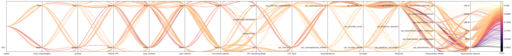
\includegraphics[width=1\linewidth]{bilder/lowlabel-paarcords-cpc-micro.png}
		\caption{The color is the \textbf{micro} ROC-AUC score}
		\label{fig:cpc-parcoords-micro}	
	\end{subfigure}
	\begin{subfigure}[t]{\textwidth}\centering
		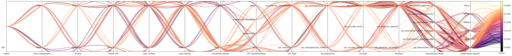
\includegraphics[width=1\linewidth]{bilder/lowlabel-paarcords-cpc.png}
		\caption{The color is the \textbf{macro} ROC-AUC score}
		\label{fig:cpc-parcoords-macro}	
	\end{subfigure}
\end{figure}


\subsubsection{Latent/Context t-SNE representations}
Does CPC learn visually verifiable useful latent representations?

In an attempt to visually verify the usefulness of the learned latent data representations we separately perform a dimensionality reduction from the 128 valued latent vectors and the 256 valued context vectors into a two dimensional space. This is done by taking one of the above trained CPC networks (with the settings use\_weights, strided, unfrozen, cpc\_downstream\_cnn in this case) and saving all latent and context vectors for the whole dataset. Afterwards we use t-SNE \autocite{JMLR:v9:vandermaaten08a} to embed the vectors into two dimensions, the results are visualized in a scatter plot where the embedded dimensions are used as x- and y-axis. Each sample is colored according to its label in the data. Since the data has multiple possible labels per sample, which makes distinct class coloring difficult, we opted to use binary coloring --- if class $x$ is present in the data assign $1$, otherwise assign $0$ to the datapoint. This is done for all classes.

In order to be able to better judge if the colored embeddings have meaning, we added a scatter plot with randomized labels as well. An example for this can be seen in \autoref{plot:tsne-context} which shows all context vector embeddings, with the labels for class $426783006$ (normal sinus rhythm). Although the data points were not fully separated, a clear distinction to the random plot can still be made (see mostly blue big area on the left). The same goes for \autoref{plot:tsne-latent} which shows all latent vector embeddings instead. There the positive labels seems to form a border around the data, the negative labels are mostly centered in the middle.
\begin{figure}[H]
	\caption{Two dimensional t-SNE embeddings of all context vectors}
	\begin{subfigure}[t]{0.48\textwidth}\centering
		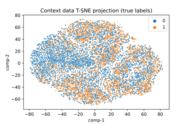
\includegraphics[width=1\linewidth]{bilder/tsne-context-41.png}
		%\caption{t-SNE embedding of all context vectors (one for each patient). Legend: }
		\label{fig:tsne-context-normal}	
	\end{subfigure}%
	\hfill	
	\begin{subfigure}[t]{0.48\textwidth}\centering
		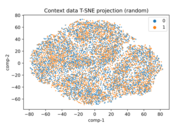
\includegraphics[width=1\linewidth]{bilder/tsne-context-(random).png}		
		\label{fig:tsne-context-random}	
	\end{subfigure}
	\caption*{t-SNE embedding of all context vectors (one for each patient). Left:  Data points are colorized according to their true labels. Right: The colors are randomly assigned.}
	\label{plot:tsne-context}
\end{figure}
\begin{figure}[H]
	\caption{Two dimensional t-SNE embeddings of all latent vectors}
	\begin{subfigure}[t]{0.48\textwidth}\centering
		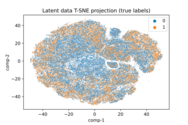
\includegraphics[width=1\linewidth]{bilder/tsne-latent-41.png}%
		%\caption{t-SNE embedding of all latent vectors (nine for each patient). Legend: $0 :=$ no normal beats (class $x:= 426783006$) are in the recordings labels, $1:=$ normal beats are in the recordings labels}
		\label{fig:tsne-latents-normal}	
	\end{subfigure}%
	\hfill	
	\begin{subfigure}[t]{0.48\textwidth}\centering
		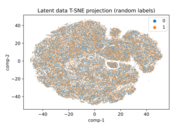
\includegraphics[width=1\linewidth]{bilder/tsne-latent-(random).png}%
		%\caption{t-SNE embedding of all latent vectors (nine for each patient). The labels $0$ and $1$ are randomly assigned.}
		\label{fig:tsne-latents-random}
	\end{subfigure}
	\caption*{t-SNE embeddings of all latent vectors (nine vectors per patient). Left: Data points are colorized according to their true labels. Right: The colors are randomly assigned.}
	\label{plot:tsne-latent}
\end{figure}

\autoref{plot:tsne-context-all} and \autoref{plot:tsne-latent-all} show the embeddings with the respective point coloring for 64 of 67 classes, denoted in the upper right of each scatter plot. The plots are ordered by their ROC-AUC-score from top-left to bottom-right, each score visualized as background color. Especially for smaller classes (fewer yellow dots) it is difficult to judge how well the data is clustered, but there are cases were clusters are clearly distinguishable. Take for example classes $427084000$ (sinus tachycardia) and $426177001$ (sinus bradycardia) in \autoref{plot:tsne-context-all}, which are on the opposite site in the embedding and also have a high ROC-AUC-score. Interestingly sinus tachycardia means that the heart beat is faster than usual (over 100bpm \autocite{SinusTachycardiaCedarsSinai-2021-09-07}) and sinus bradycardia that the heart beats slower than usual (under 60bpm \autocite{SinusBradycardiaCedarsSinai-2021-09-07}), which means the classes are in fact conflicting and very unlikely to occur together as final diagnosis on the same patient. The same classes are also fairly spatially divided with the latent embeddings \autoref{plot:tsne-latent-all}, however not as clearly as with the context embeddings. This might be due to the fact that a patient diagnosed with sinus tachycardia might still have a few slow beats or vice versa with sinus bradycardia. Also since the tested model relies on the context vector for the final prediction, the classes need to be more distinguishable in the context vector space than the latent vector space, which could explain the better spatial division. Additionally since nine times more latent data points are generated, the two dimensional embedding could be harder to find for t-SNE.

In contrast to spatially divided clusters there also seem to be class clusters which are more or less equivalent. In \autoref{plot:tsne-latent-all} take for example classes $6374002$ (Bundle Branch Block) and $164909002$ (Left Bundle Branch Block), which look very similar apart of their sizes, and are also very similar from a medical standpoint.
\begin{figure}[H]
	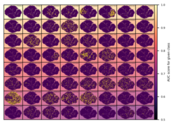
\includegraphics[height=\linewidth, angle=90]{bilder/tsne-context-all(ordered by auc).png}
	\caption[Two dimensional t-SNE embeddings of all context vectors]{t-SNE embedding of all context vectors (one for each patient) for 64 of 67 classes. Legend: number in top right denotes class name, yellow dot means class name is part of the recording's labels. Background color is the AUC score per class, sorted descending}
	\label{plot:tsne-context-all}
\end{figure}
\begin{figure}[H]\centering
	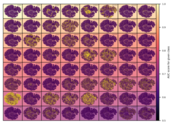
\includegraphics[height=\linewidth, angle=90]{bilder/tsne-latent-all(ordered by auc).png}
	\caption[Two dimensional t-SNE embeddings of all latent vectors]{t-SNE embedding of all latent vectors (nine for each patient) for 64 of 67 classes. Legend: number in top right denotes class name, yellow dot means class name is part of the recording's labels. Background color is the AUC score per class, sorted descending}
	\label{plot:tsne-latent-all}
\end{figure}

\begin{figure}[H]\centering
	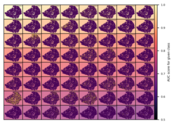
\includegraphics[height=\linewidth, angle=90]{bilder/tsne-context-all(ordered by auc)new.png}
	\caption[Two dimensional t-SNE embeddings of all context vectors (different model)]{t-SNE embedding of all context vectors (one for each patient) for 64 of 67 classes. Context obtained with frozen model. Legend: number in top right denotes class name, yellow dot means class name is part of the recording's labels. Background color is the AUC score per class, sorted descending}
	\label{plot:tsne-context-all-frozen}
\end{figure}
\begin{figure}[H]\centering
	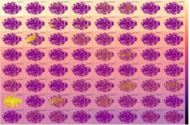
\includegraphics[height=\linewidth, angle=90]{bilder/tsne-latent-all2(ordered by auc).png}
	\caption[Two dimensional t-SNE embeddings of all latent vectors (different model)]{t-SNE embedding of all latent vectors (26 for each patient) for 64 of 67 classes. Latents obtained with frozen model. Legend: number in top right denotes class name, yellow dot means class name is part of the recording's labels. Background color is the AUC score per class, sorted descending.}
	\label{plot:tsne-latent-all-frozen}
\end{figure}

We compare prior results of a strided model where all weights are updated, with the t-SNE embeddings of a non-strided network that was trained with frozen weights. As a result the learned latent representations obtained by only the CPC loss are formed completely independent of labeled data. The t-SNE embeddings will show how/if the latents are dividable into clusters and if the highlighted classes are comparably separable. 

\autoref{plot:tsne-context-all-frozen} shows the t-SNE embedding of the context vectors, while \autoref{plot:tsne-latent-all-frozen} shows the embedding for all latent vectors. Comparing the different model's context plots, we notice that the true samples of that specific class (yellow dots) seem to be less grouped and more spread throughout the plot. The distinction we made in the first plot between class sinus tachycardia and sinus bradycardia cannot be made anymore. We suspect that the training with updated weights is important for building a context that is focused on predicting class labels, rather than the next latent steps.

On the other side, for the latent embedding we observe that there seems to be a way finer clustering in general, which are however not restricted to class labels. We argue that the latent representations formed in the model with frozen weights have distinct properties partly independent of their class label in the data, which is not surprising as the CPC loss is minimized without labels. The class labels seem to appear predominantly in few selected clusters which suggests that each class has its own defining properties.

In conclusion the context vectors of the strided model with updated weights seems to be more suited for classification, while the latent representations of the frozen non-strided model appear to be of higher quality and more capable of identifying unique data properties, which are focused on specfic classes only sporadically.
This suggests that CPC finds general latent representations which encode the data's properties and that during the downstream task those representations get fine tuned for classification. In the case of the strided model those representations were less separable in a lower dimension, where It's not entirely clear if these properties got imperfectly "mixed" into classes, or if the strided model's latent representations have less distinct properties in general.

\subsubsection{Transforming Predictions Scores with Model Thresholds}
After predictions for the ECG-data have been made it is important to visualize them correctly, to give an idea of what class labels are considered true
Let $p$ be a prediction score vector for $n$ classes $p=(s_1,\ldots,s_n)$ with $\forall i\leq n: s_i\in[0, 1]$ and $t$ be a threshold score vector for $n$ classes $t=(t_1,\ldots,t_n)$ with $\forall i\leq n: t_i\in[0, 1]$ that decides if class $i$ is considered true (\autoref{eqn:thresh}). We define the reweighted probability scores $p_r=(r_1, \ldots, r_i, \ldots, r_n)$ as:
\begin{equation}
	r_i:=
	\begin{cases}
		(\frac{s_i-t_i}{t_i}+1)/2,& \text{if } s_i < t_i\\
		(\frac{s_i-t_i}{1-t_i}+1)/2,& \text{if } s_i \geq t_i\\
	\end{cases}
	\label{eqn:rew-probs}
\end{equation}
The reweighting function can be explained as splitting scores into positive and negative predictions where we stretch the space below the threshold $[0, t_i[$ to $[0, 0.5[$ and the space above and equal to threshold $t_i$: $[t_i, 1] \mapsto [0.5, 1]$. This has the advantage that predictions mean the same across all classes and models: We moved the decision boundary from $\forall{i}, t_i\mapsto0.5$ In \autoref{fig:scatter1} and \autoref{fig:scatter2} we see examples for the process of transforming  model outputs to reweighted probabilities.

\subsubsection{Hand-picked Samples: Prediction Score Scatterplots}

\begin{figure}[H]
	\caption{Scatterplots showing from left to right: exact model predictions, model predictions minus specific class thresholds, reweighted prediction probabilities}
	\begin{subfigure}[t]{0.95\textwidth}\centering
		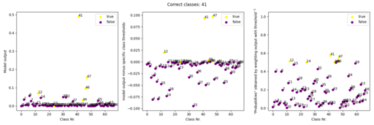
\includegraphics[width=1\linewidth]{bilder/HR04093scatterplot-predictions(combined)}
		\caption{CPC Model}
		%\label{fig:bl-parcoords-micro}	
	\end{subfigure}%
	
	\begin{subfigure}[t]{0.95\textwidth}\centering
		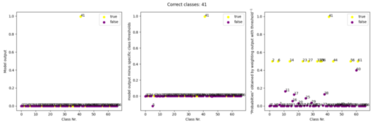
\includegraphics[width=1\linewidth]{bilder/HR04093scatterplot-predictions(combined)bl14}
		\caption{Baseline Model (BL\_v14)}
		%\label{fig:bl-parcoords-micro}	
	\end{subfigure}%
	\label{fig:scatter1}
\end{figure}
Looking at the leftmost plot in \autoref{fig:scatter1}, we see why reweighting probabilities is important for readability: the unchanged model outputs for class $44$ is considered true by the model but has a lower probability output than for example class 6 which is considered false. We substract the class specific thresholds and obtain a more readable output. Last but not least we transform the differences into real probabilities and are even able to judge how sure a model is about specific predictions: the closer to $0$ or $1 \implies$ prediction certainty high.

For the \code{BL\_v14} model predictions we observe that only the correct class $41$ has a high probability of being true while the other classes falsely classified as true barely go above $0.5$. The CPC model predictions are less confident in general, however class 41 has still the highest probability. At this place we also want to point out a flaw of scores that are based on binary predictions: In this specific case CPC would have the higher score, as fewer classes are wrongly classified as true. Nevertheless we make the argument that in this case the predictions of the \code{BL\_v14} are higher quality because of the models high certainty prediction of the correct class.

\autoref{fig:scatter2} shows yet another prediction example --- this time we would argue that the CPC predictions are slightly better, at least concerning classes labeled "true". Although more classes are classified as true erroneously, both $33$ and $41$ have been predicted with the highest certainty. Compare this to The baseline predictions where $41$ is fairly certain, but $33$ is just as unlikely as erroneously classified classes.
\begin{figure}
	\caption{Scatterplots showing from left to right: exact model predictions, model predictions minus specific class thresholds, reweighted prediction probabilities}
	\begin{subfigure}[t]{0.95\textwidth}\centering
		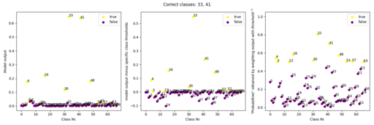
\includegraphics[width=1\linewidth]{bilder/HR04811scatterplot-predictions(combined).png}
		\caption{CPC Model}
		%\label{fig:bl-parcoords-micro}	
	\end{subfigure}	
	\begin{subfigure}[t]{0.95\textwidth}\centering
		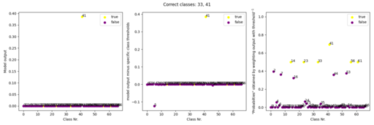
\includegraphics[width=1\linewidth]{bilder/HR04811scatterplot-predictions(combined)bl14.png}
		\caption{Baseline Model (BL\_v14)}
		%\label{fig:bl-parcoords-micro}	
	\end{subfigure}%
	\label{fig:scatter2}
\end{figure}

%\subsubsection{All Samples: Errorbars for Average Model Prediction Scores}
%\begin{figure}
%	\caption{Errorplot showing the exact model predictions, divided into groups depending on their ground truth label.}
%	\begin{subfigure}[t]{0.95\textwidth}\centering
%		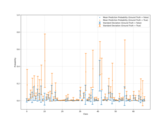
\includegraphics[width=1\linewidth]{bilder/errorplot-prediction-cpc.png}
%		\caption{Errorplot for CPC model}
%		%\label{fig:bl-parcoords-micro}	
%	\end{subfigure}
%	\begin{subfigure}[t]{0.95\textwidth}\centering
%		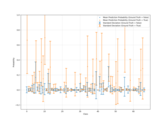
\includegraphics[width=1\linewidth]{bilder/errorplot-prediction-blv15.png}
%		\caption{Errorplot for Baseline (v15) model}
%		%\label{fig:bl-parcoords-micro}	
%	\end{subfigure}%
%	\label{fig:errorplot}
%\end{figure}
%\autoref{fig:errorplot} shows the averaged model predictions for all classes and their corresponding standard deviation. The predictions are divided into two groups, where blue states the ground truth class label for the input data is True, whereas orange states the label is false.
%
%In the baseline plot, the average probability of negative samples are below the means of the positive samples in most cases, which shows the model predicts the class labels correctly on average. Nevertheless it is noticeable that predictions where the ground truth is true are wider spread than where the ground truth is false and also that there are intersections between the two groups in which fully correct predictions are impossible to make.
%
%For the CPC model, similar observations can be made, with the difference that most average values are lower than in the baseline plot and the standard deviations are closer to the mean as well.
%
%However before jumping to conclusion we need to utilize the class thresholds that were obtained by maximizing the ROC-AUC (\autoref{sec:evaluation}) to reweight the model outputs to make them comparable and obtain values that are more spread in $[0, 1]$.
%
%\autoref{fig:errorplot-threshold} and \autoref{fig:errorplot-threshold-meangap} show these reweighted errorplots, where the latter is additionally sorted by the difference between the group class prediction averages, which is a further effort to make them comparable more easily. 
%\begin{figure}
%	\caption{Errorplot showing the model predictions reweighted with the corresponding class thresholds}
%	\begin{subfigure}[t]{0.48\textwidth}\centering
%		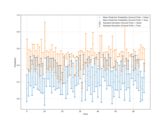
\includegraphics[width=1\linewidth]{bilder/errorplot-prediction-threshold-cpc.png}
%		\caption{Errorplot for CPC model}
%		%\label{fig:bl-parcoords-micro}	
%	\end{subfigure}%
%	\hfill
%	\begin{subfigure}[t]{0.48\textwidth}\centering
%		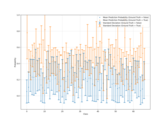
\includegraphics[width=1\linewidth]{bilder/errorplot-prediction-threshold-blv15.png}
%		\caption{Errorplot for Baseline (v15) model}
%		%\label{fig:bl-parcoords-micro}	
%	\end{subfigure}%
%	\label{fig:errorplot-threshold}
%\end{figure}
%\begin{figure}
%	\caption{Errorplot showing the model predictions reweighted with the corresponding class thresholds (sorted by gap between group averages)}
%	\begin{subfigure}[t]{0.95\textwidth}\centering
%		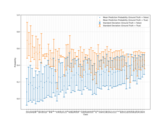
\includegraphics[width=1\linewidth]{bilder/errorplot-prediction-threshold-cpc-meangap.png}
%		\caption{Errorplot for CPC model, sorted by gap between means}
%		%\label{fig:bl-parcoords-micro}	
%	\end{subfigure}	
%	\begin{subfigure}[t]{0.95\textwidth}\centering
%		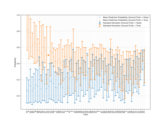
\includegraphics[width=1\linewidth]{bilder/errorplot-prediction-threshold-blv15-meangap.png}
%		\caption{Errorplot for Baseline (v15) model, sorted by gap between means}
%		%\label{fig:bl-parcoords-micro}	
%	\end{subfigure}%
%	\label{fig:errorplot-threshold-meangap}
%\end{figure}
%
%To show that model predictions are not evenly distributed we visualize the standard deviations "in two directions" --- one shows the mean squared difference from the prediction mean above the prediction mean, the other shows the mean squared difference from the prediction mean below the mean. Again, it's hard to draw a clear conclusion concerning which of the models is performing better, but we argue that the CPC models predictions seem to be less overlapped and thus binary predictions will be more accurate.
%\begin{figure}
%	\caption{Errorplot showing the model predictions reweighted with the corresponding class thresholds (sorted by gap between group averages)}
%	\begin{subfigure}[t]{0.95\textwidth}\centering
%		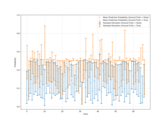
\includegraphics[width=1\linewidth]{bilder/errorplot-prediction-threshold-cpc-twodirectional.png}
%		\caption{Errorplot for CPC model, with std calculated  "in two directions"}
%		%\label{fig:bl-parcoords-micro}	
%	\end{subfigure}%
%	
%	\begin{subfigure}[t]{0.95\textwidth}\centering
%		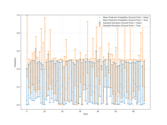
\includegraphics[width=1\linewidth]{bilder/errorplot-prediction-threshold-blv15-twodirectional.png}
%		\caption{Errorplot for Baseline (v15) model, with std calculated  "in two directions"}
%		%\label{fig:bl-parcoords-micro}	
%	\end{subfigure}%
%	\label{fig:errorplot-threshold-twodir}
%\end{figure}

\subsubsection{All Samples: Violinplots}
Below in \autoref{fig:violinplot-normal} we include the raw prediction score data visualized as a violinplot, which show the prediction distributions for all classes. We opted to visualize both True and False prediction distributions with the same width, which removes the information about the group sizes, but increases readability. Noticeable is that even without the reweighting of model predictions, probabilities in the baseline model are more evenly distributed within $[0,1]$, indicating that the sigmoid was able to more precisely predict the extrema $0$ and $1$. This is not implicitly better since thresholds get selected to divide the probabilties into true and false anyways and as long as the false and true label predictions are more or less separate from each other, results are equally correct.
%\begin{figure}[H]
%	\caption{Scatterplot showing all exact model predictions, divided into groups depending on their ground truth label.}
%	\begin{subfigure}[t]{0.5\textwidth}\centering
%		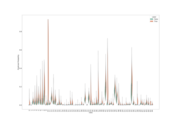
\includegraphics[width=1\linewidth]{bilder/cpc-probdistribution-unfrozen-standard-width.png}
%		\caption{Scatterplot for a CPC model; unfrozen during Downstream Training. Horizontal lines show model specific decision thresholds}
%		%\label{fig:bl-parcoords-micro}	
%	\end{subfigure}
%	\begin{subfigure}[t]{0.5\textwidth}\centering
%		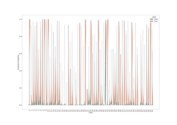
\includegraphics[width=1\linewidth]{bilder/bl-probdistribution-standard-width.png}
%		\caption{Scatterplot for Baseline (v14) model. Horizontal lines show model specific decision thresholds}
%		%\label{fig:bl-parcoords-micro}	
%	\end{subfigure}%
%	
%	\begin{subfigure}[t]{0.5\textwidth}\centering
%		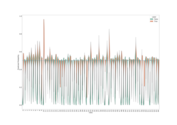
\includegraphics[width=1\linewidth]{bilder/cpc-probdistribution-unfrozen-reweighted-width.png}
%		\caption{Scatterplot for CPC model; unfrozen during Downstream Training. Probabilities reweighted as per \autoref{eqn:rew-probs}}
%		%\label{fig:bl-parcoords-micro}	
%	\end{subfigure}%
%	\begin{subfigure}[t]{0.5\textwidth}\centering
%		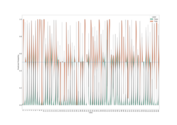
\includegraphics[width=1\linewidth]{bilder/bl-probdistribution-reweighted-width.png}
%		\caption{Scatterplot for Baseline (v14) model. Probabilities reweighted as per \autoref{eqn:rew-probs}}
%		%\label{fig:bl-parcoords-micro}	
%	\end{subfigure}%
%	\label{fig:errorplot-scatter-all}
%\end{figure}
\begin{figure}[H]
	\caption{Scatterplot showing all exact model predictions, divided into groups depending on their ground truth label.}
	\begin{subfigure}[t]{1\textwidth}\centering
		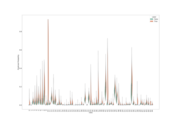
\includegraphics[width=1\linewidth]{bilder/cpc-probdistribution-unfrozen-standard-width.png}
		\caption{Violinplot for a CPC model; unfrozen during Downstream Training. Horizontal lines show model specific decision thresholds}
		%\label{fig:bl-parcoords-micro}	
	\end{subfigure}
	\begin{subfigure}[t]{1\textwidth}\centering
		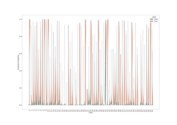
\includegraphics[width=1\linewidth]{bilder/bl-probdistribution-standard-width.png}
		\caption{Violinplot for Baseline (v14) model. Horizontal lines show model specific decision thresholds}
		%\label{fig:bl-parcoords-micro}	
	\end{subfigure}%
\label{fig:violinplot-normal}
\end{figure}
Yet again, with the model thresholds added in \autoref{fig:violinplot-reweight}, the groups are more or less visibly split into true and false samples, with some exceptions like class 41 (sinus rythm), where true samples get classified as false or false samples as true fairly often. The comparison between CPC model and baseline model is difficult, but we notice that "False" classes are more oftenly wrongly classified as true for the CPC model. Interesting to see is that both models failed to predict class 36 correctly, where the baseline model even predicted samples as false with high certainty ($p=0$). On the other side these plots also show strengths of specific models: Class 31 is correctly split into true and false samples for the baseline model but not the CPC model, whereas class 62 is correctly classified by CPC but not the baseline. Looking at the class distribution in \autoref{fig:ClassCountsBar} we observe that class 62 is a small class only available in select datasets, again hinting at CPC's ability of needing less labeled data.

With the help of these plots one could create a model ensemble which utilizes different networks for each class, creating a more powerful and accurate prediction model.
\begin{figure}[H]	
	\begin{subfigure}[t]{1\textwidth}\centering
		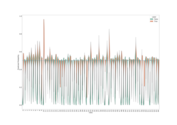
\includegraphics[width=1\linewidth]{bilder/cpc-probdistribution-unfrozen-reweighted-width.png}
		\caption{Violinplot for CPC model; unfrozen during Downstream Training. Probabilities reweighted as per \autoref{eqn:rew-probs}}
		%\label{fig:bl-parcoords-micro}	
	\end{subfigure}
	\begin{subfigure}[t]{1\textwidth}\centering
		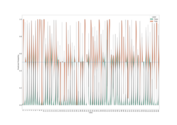
\includegraphics[width=1\linewidth]{bilder/bl-probdistribution-reweighted-width.png}
		\caption{Violinplot for Baseline (v14) model. Probabilities reweighted as per \autoref{eqn:rew-probs}}
		%\label{fig:bl-parcoords-micro}	
	\end{subfigure}%
\label{fig:violinplot-reweight}
\end{figure}

\subsubsection{Explaining predicted classes in input data}\label{sec:explainingclasses}
As a bonus, having predicted a diagnostic label, it might be of great interest to also highlight where the model assumes the predicted classes are located at in the input data. We try to accomplish this task by performing a feed-forward of the input data through the network and than calculate the loss between the prediction and the target $y^c$ --- an all-zero valued vector ($\sim$ all diagnostic labels have a probability of 0) besides a specified target class $c$ , which is set to one (class probability $1$). As of yet we use the available ground truth labels, which are, if not available, to be replaced with the binary predictions obtained with the model's thresholds. The gradients are calculated by backpropagation with respect to the input data $X$. Once the gradient matrices $\frac{\partial y^c}{\partial X}$ has been obtained, we either take their absolute values to visualize areas that have an impact in general or apply a ReLU activation to highlight areas that positively influence the target's class prediction. The latter idea is based on the Grad-CAM paper \autocite{DBLP:journals/corr/SelvarajuDVCPB16}, the procedure in general is called guided backpropagation \autocite{HowtoVisuallyExplainanyCNNbasedModelsbyRenuKhandelwalTowardsDataScience-2022-01-18}. We normalize the matrices individually to $[0, 1]$ and assign colors for each class, which increase in opacity for high values and become transparent below a certain threshold (e.g. $<0.2$, which varies depending on model). We can see what values in the data would have to change in order to decrease the loss: High gradient values $\sim$ high influence on the predicted classes; low gradient values $\sim$ less influence on the predicted classes. To show multiple classes/colors in the same spots we divide the ecg channels into the number of present classes and color each division separately. The final result with multiple patients as example can be seen in \autoref{explain-bl} for the \code{BL\_v8} model and in \autoref{explain-cpc} for a CPC Model. 

\begin{figure}
	\begin{subfigure}{1\textwidth}\centering
		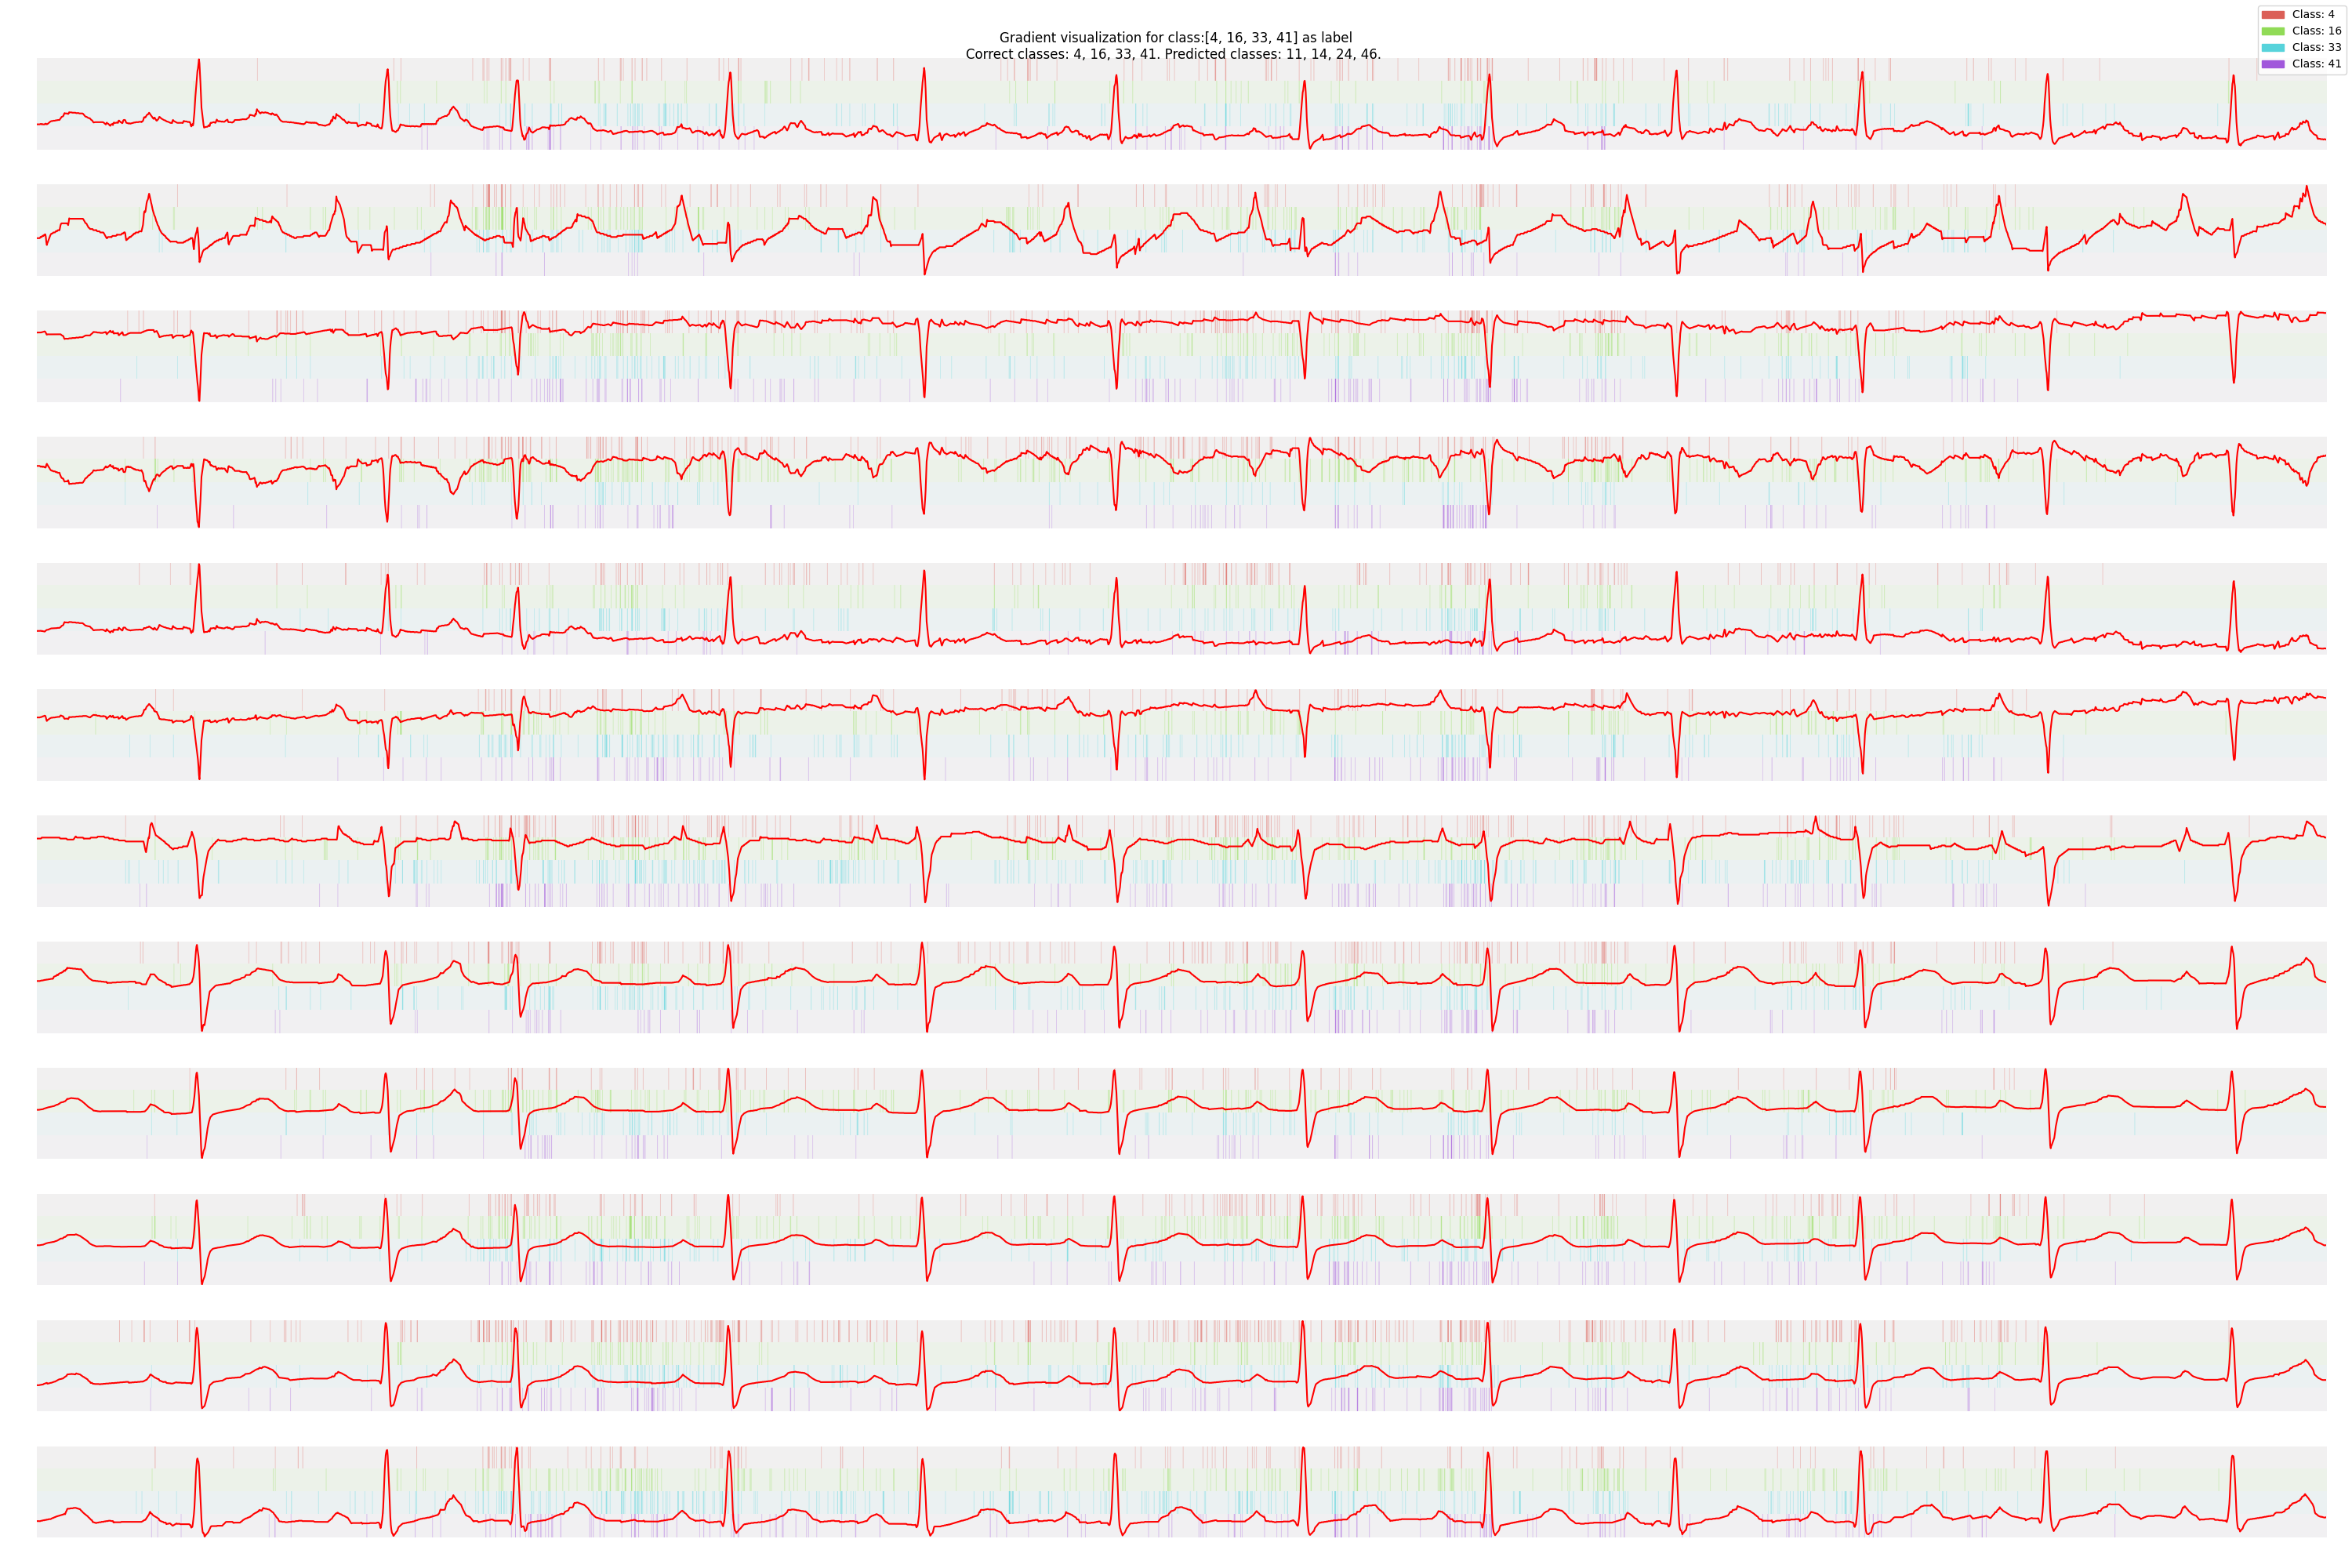
\includegraphics[width=\linewidth]{"bilder/HR07448-class:[4, 16, 33, 41]-gradient-cambl11.png"}
		\caption{ECG example HR07448}
		%\label{explain}
		\centering
	\end{subfigure}
	\begin{subfigure}{1\textwidth}\centering
		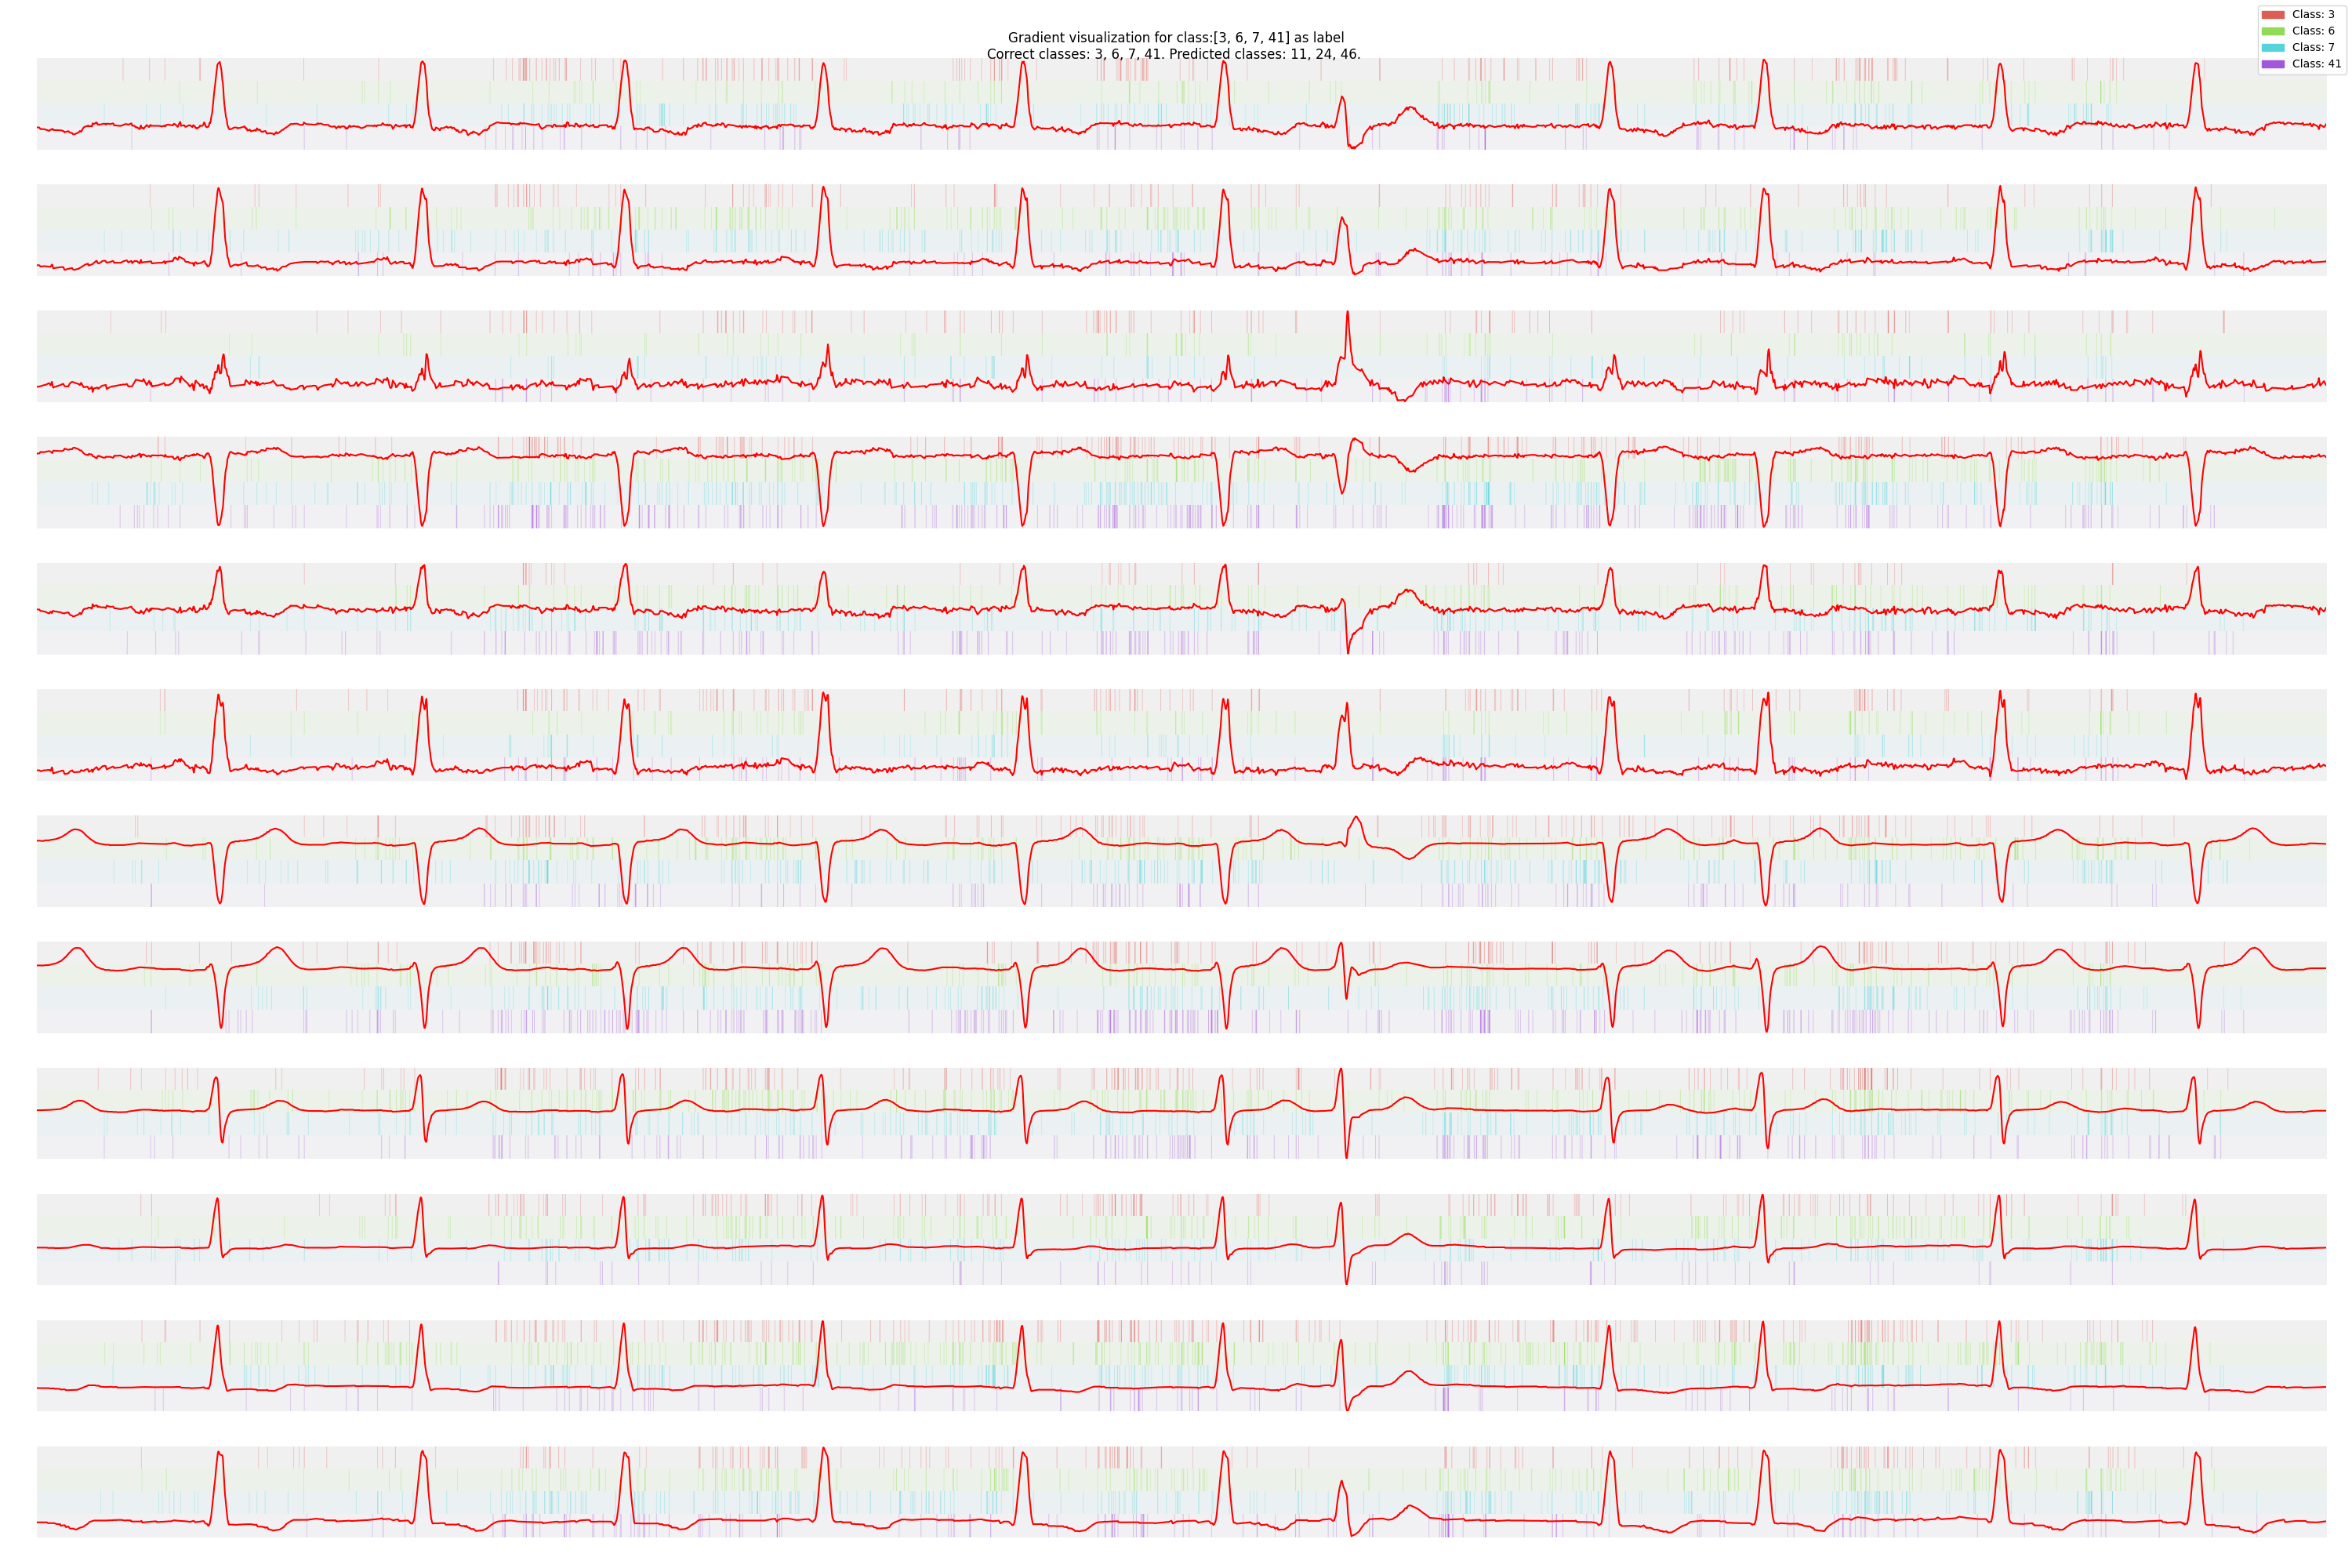
\includegraphics[width=\linewidth]{"bilder/HR16414-class:[3, 6, 7, 41]-gradient-cambl11.png"}
		\caption{ECG example HR16414}
		%\label{explain}
		\centering
	\end{subfigure}
	\caption{\code{BL\_v8} model gradients. Absolute gradient values utilized. Colored vertical bars/areas show "interesting/controversial" spots in the input data.}
	\label{explain-bl}
\end{figure}
\begin{figure}
	\begin{subfigure}{1\textwidth}\centering
		\includegraphics[width=\linewidth]{"bilder/HR07448-class:[4, 16, 33, 41]-gradient-camcpc2.png"}
		\caption{ECG example HR07448}
		%\label{explain}
		\centering
	\end{subfigure}
	\begin{subfigure}{1\textwidth}\centering
		\includegraphics[width=\linewidth]{"bilder/HR16414-class:[3, 6, 7, 41]-gradient-camcpc2.png"}
		\caption{ECG example HR16414}
		%\label{explain}
		\centering
	\end{subfigure}
	\caption{CPC model (with \code{encoder\_v0}) gradients. Absolute gradient values utilized. Colored vertical bars/areas show "interesting/controversial" spots in the input data.}
	\label{explain-cpc}
\end{figure}
Interestingly the CPC model's biggest gradient values are less spread throughout the input which could potentially lead to marking interesting spots with a higher precision. On the other hand locations might not get marked although classes are present there. The markings in the baseline model are almost everywhere, making class judgments more difficult.


Additionally to our approach of calculating $\frac{\partial y^c}{\partial X}$, we tested Grad-CAM \autocite{DBLP:journals/corr/SelvarajuDVCPB16} which takes the gradient $\frac{\partial y^c}{\partial A^k}$ of the convolutional feature maps $A^k$ in a selected layer and calculates $L^c_{\mathrm{Grad-CAM}} = \mathit{ReLU}\left(\sum_{k}\alpha^c_k A^k\right)$, where $\alpha^c_k=\frac{1}{ij}\sum_i\sum_j\frac{\partial y^c}{\partial A^k_{i,j}}$ is the mean/ global average pooling of feature map $A^k$. $L^c_{\mathrm{Grad-CAM}}$ can thus be seen as the sum of all feature maps in a specified layer, weighted according to their importance in predicting a specified class $c$, which results in a coarse heatmap where the model assumes the class to be located. One big upside compared to our localization approach is that the locations are directly generated from later layers, where most class features are encoded in. The downside however is that the heatmap size is dependent on the individual architecture and not the input data. This leads to few values available for localization in some cases. Additionally, in contrast to our approach, all channel information get lost, meaning eg. ecg-channel v1 and ecg-channel v3 are colored the exact same, although a specific class can only be recognized in one of them.

The coarse heatmap is then rescaled to match the input size, which is $4500$ in our case. Since the layers feature map channels get summarized into a single value, no spots depending on input channels can be recovered and all input channels share the same areas of interest. This is to say that even if a certain class is only visible in a specific ecg channel all others will be colorized as well, which is a clear downside to our approach. Furthermore the heat map's size is dependent on the downsampling factor in the data dimension of the model architecture: For our \code{encoder\_v0} CPC model only $1\times26$ values are generated, which allows for a rough localization of classes in the input data only. The BL\_v8 model generates $1\times147$ values which results in much finer localization in the input data and thus more accurate results. The \code{TCN\_down} architecture is probably the most interesting one since it makes use of heavy padding and no strides, making it output $4500$ values (same as input) even in the later layers. We expect the best results there.

\begin{figure}
	\begin{subfigure}{1\textwidth}\centering
		\includegraphics[width=\linewidth]{"bilder/HR07448-class:[4, 16, 33, 41]-gradient-cambl8.png"}
		%\label{explain}
		\centering
	\end{subfigure}	
	\caption{ECG examples, for the BL\_v8 Model, Grad-Cam technique used. 147 feature map values stretched to input length of 4500.}
	\label{explain-gradcam-v8}
\end{figure}
In \autoref{explain-gradcam-v8} we see that Grad-Cam created spots in the data that might be able to successfully explain the classes position in the input data. For example the normal sinus rhythm (no. 41) can be found in regular intervals everywhere in the data as expected, while "Left Axis Deviation" (class 33) can only be found at a single spot. "Mycardial Infarction" (class 4) is assumed at 2-3 spots.

\begin{figure}
	\begin{subfigure}[t]{1\textwidth}\centering
		\includegraphics[width=\linewidth]{"bilder/HR07448-class:[4, 16, 33, 41]-gradient-camcpc0.png"}
		\caption{\code{encoder\_v0} used. 26 feature map values stretched to input length of 4500.}
		\label{explain-gradcam-cpcv0}
		\centering
	\end{subfigure}
	\begin{subfigure}[t]{1\textwidth}\centering
		\includegraphics[width=\linewidth]{"bilder/HR07448-class:[4, 16, 33, 41]-gradient-camcpc8.png"}
		\caption{\code{encoder\_likev8} used. 147 feature map values stretched to input length of 4500.}
		\label{explain-gradcam-cpclikev8}
		\centering
	\end{subfigure}	
	\caption{ECG examples, for the CPC Model, Grad-Cam technique used.}
\end{figure}
For CPC model \autoref{explain-gradcam-cpcv0} we see that the grad-cam results are not very localized and all over the place, also the different classes do not seem to differ between one another. We compare to a CPC model that is trained with a different encoder to check whether the poor performance is always present: \autoref{explain-gradcam-cpclikev8}. We observe similar results as with the baseline model.

\begin{figure}
	\begin{subfigure}{1\textwidth}\centering
		\includegraphics[width=\linewidth]{"bilder/HR07448-class:[4, 16, 33, 41]-gradient-camtcn.png"}
		%\label{explain}
		\centering
	\end{subfigure}	
	\caption{ECG examples, for the TCN (down) architecture, Grad-Cam technique used. 4500 feature map values 'stretched' to input length of 4500.}
	\label{explain-gradcam-tcn}
\end{figure}
The \code{TCN} baseline model in \autoref{explain-gradcam-tcn} has a very clear localization of classes, which is probably mostly due to the big output size even in later layers, since the \code{v8} network has a similar macro average score.


Last but not least we asked a cardiologist to rate the class markings in the grad-cam images and we were given the following comments:
\begin{itemize}
	\item In \autoref{explain-gradcam-v8} the sinus rhythm (class 41) is off place in some places and generally too spread out. When labeling it you would pick the center of the QRS-points
	\item \autoref{explain-gradcam-cpcv0} is marking too much, no specific locations are clearly recognizable.
	\item In \autoref{explain-gradcam-cpclikev8} the sinus rhythm is again off beat in some places but otherwise recognizable. The myocardial infarction is diagnosed mostly by looking at the S-T interval, which is also marked here. Left axis deviation is a "turned-around" QRS complex, so the localization seems okay, but should only be marked in selected channels (eg. channel 3).
	\item \autoref{explain-gradcam-tcn} perfectly shows the sinus rhythm center at the QRS complex but disregards the P-wave completely. The myocardial infarction is not diagnosed by looking at the QRS complex, making these markings probably incorrect. Left axis deviation is visible in some channels only, but all got marked.
\end{itemize}
When asked to pick a "best-performing" figure they selected \autoref{explain-gradcam-cpclikev8}. 

Especially the fact that some classes are only visible in certain channels shows that the grad-cam technique is intended for use on images where different data channels encode color but have no independent role in localizing different classes. Calculating the gradient towards the input does not share this drawback but the gradient is not as suited for localizing class labels. We tried "Guided-Grad-Cam" which in our case struggled to display anything at all, since guided backpropagation and gradient cam are multiplied to receive the final output, the image was almost always mostly without colors due to values close to $0$.



\section{Discussion and Future work} \label{sec:discussion}

In a fully supervised setting, our baselines were able to produce slightly better prediction results compared to our Contrastive Predictive Coding models. Once we handicapped CPC by splitting the training into a pretraining and downstream training phase, with the same number of epochs given in total, the advance for the baseline models increased even further. Yet the CPC results were still above average.

Thus, when labels are available in large enough quantities, supervised learning methods, that have seen much research in the past, are probably easier to optimize and are able to produce better results as a consequence.

In environments where only few labels are given, which we tried to emulate in our "Low Label Availability" experiment in \autoref{section:lowlabel}, CPC showed better results compared to baseline models, when the least labels were given, after allowing sufficient training epochs. This is an indicator that CPC pretraining can improve classification results in fields where unlabeled data is readily available, while high quality labels are rare and only obtainable with high costs and effort --- which is the case in many fields of modern medicine.

Furthermore our augmented/noised data experiment in \autoref{sec:augmented} suggests that CPC pretraining increases training stability in the downstream task for unbalanced datasets, because both baseline- and the CPC networks that were trained fully supervised, mostly failed to classify the data satisfactory.

An additional strong benefit of CPC is time efficiency. Downstream tasks, where one has to train models with the same input data, but different labels, benefit of the shared  weights obtained during pretraining. Often CPC can yield good results with only few downstream epochs, reducing the necessary total training time drastically. This especially showed during training on the different train splits in "Low Label Availability" experiment: while the baselines were trained completely from ground up for every split, needing more than 24 hours wall clock time, the CPC models were trained in a fraction of that time.

CPC allows for many architectural choices, for example the encoder network and many hyperparameters like latent-size, context-size, number of summarized latents, number of predicted latents and the latent sampling method to name just a few. This makes it very flexible and applicable to many data modalities, as it does not make explicit demands on label shapes and does not require pseudo-labels like many other representation learning algorithms mentioned in the introduction, making it a strong contender for universal representation learning. This also shows in the original paper, where CPC was applied to multiple data modalities, such as images, timeseries or even reinforcement learning\autocite{DBLP:journals/corr/abs-1807-03748}. However the great flexibility might also bear the risk of finding only suboptimal network settings for your specific task. This can also be seen in our implementation \autoref{sec:additionalchanges}, where we showed that a context network is not even required to learn useful representations, but also that changing the encoder resulted in worse classification results, albeit giving more flexibility to the user.

Last but not least we applied grad-cam \autocite{DBLP:journals/corr/SelvarajuDVCPB16} to selected ECG samples, where a CPC network using our \code{cpc\_encoder\_likev8} encoder module, was voted the visually best performing network by a cardiologist.

In conclusion we infer that Contrastive Predictive Coding is an overall good method for classifying ECG-data, but for the pure classification task our baseline models that were trained purely supervised performed better and should be used instead. CPC networks' strengths can be seen when only few labels are available or the data is noisy, but we had to artificially create these environments for the ECG data to outperform the baseline models. CPC yielded the best results in our colorization task, which are however still far from perfect.

Future work might include the search for additional representation learning methods that also cope well with timeseries/sequential/non-image data. This includes the aforementioned altered CPC architectures, but also unrelated representation learning networks like VQ-VAE or more simple encoder-decoder architectures.

Additionally the findings of \autocite{song2020multilabelcontrastive} show that the original CPC has a high bias and needs a lot of negative samples to correctly approach the mutual information value. They introduce a revised CPC called $\alpha$-CPC that uses weights on both positive and negative samples. According to their formulation the original CPC then becomes a special case of $\alpha$-CPC. They also introduced a method called "Multi-label Contrastive Predictive Coding" where multiple positive samples are used to greatly decrease the theoretically needed amount of negative samples. Their conducted experiments showed a superior mutual information estimation and slightly better accuracy overall. We tried to reimplement $\alpha$-CPC but our networks failed to decrease the loss satisfactory. Correctly reproducing their findings could potentially lead to better results in our experiments. 



%%%%%%%%%%%%%%%%%%%%%%%%%%%%%%%%%%%%%%%%%%%%%%%%%%%%%%%%%%%%%%%%%%%%%%%%
%%%% ENDE TEXTTEIL %%%%%%%%%%%%%%%%%%%%%%%%%%%%%%%%%%%%%%%%%%%%%%%%%%%%%
%%%%%%%%%%%%%%%%%%%%%%%%%%%%%%%%%%%%%%%%%%%%%%%%%%%%%%%%%%%%%%%%%%%%%%%%

\clearpage

% Entfernen Sie das Kommentar aus der nachfolgenden Zeile, falls Sie einen Anhang in der Arbeit verwenden wollen. Beachten Sie, dass Sie sich im Verlauf der Arbeit mit \ref{...} (z.B. \ref{anhang:zusatz1}) auf den Anhang beziehen.
%\newpage
\appendix
\section{Appendix} \label{appendix}
%
%%\begin{figure}[h]
%%	\includegraphics[width=0.8\textwidth]{bilder/ROC-multiclass.png}
%%	\caption{Example for a ROC-Curve obtained during evaluation. The numbers in the legend are the \textit{SNOMED} codes for the classes. Micro and Macro are the averages along the classes.}
%%	\label{fig:roc-example}
%%	\centering
%%\end{figure}
%
%\subsection{Baseline Results}
%\begin{figure}
%	\captionof{table}{Baseline F1 scores}
%	\begin{subfigure}[b]{0.49\hsize}\centering
%		\input{"/home/julian/Downloads/Github/contrastive-predictive-coding/models/25_06_21-16-test|bl_FCN+bl_MLP+bl_TCN_block+bl_TCN_down+bl_TCN_flatten+bl_TCN_last+bl_alex_v2+bl_cnn_v0+bl_cnn_v0_1+bl_cnn_v0_2+bl_cnn_v0_3+bl_cnn_v1+bl_cnn_v14+bl_cnn_v15+bl_cnn_v2+bl_cnn_v3+bl_cnn_v4+bl_cnn_v5+bl_cnn_v6+bl_cnn_v7+bl_cnn_v8+bl_cnn_v9+/f1-scores-avg-dataloader0.tex"}
%		\caption{Models trained with class weights in the loss function.}
%		\label{tbl:f1scores-avg-bl-class}	
%	\end{subfigure}%
%	\begin{subfigure}[b]{0.49\hsize}\centering
%		\input{"/home/julian/Downloads/Github/contrastive-predictive-coding/models/26_06_21-15-test|(2x)bl_MLP+bl_FCN+bl_TCN_block+bl_TCN_down+bl_TCN_flatten+bl_TCN_last+bl_alex_v2+bl_cnn_v0+bl_cnn_v0_1+bl_cnn_v0_2+bl_cnn_v0_3+bl_cnn_v1+bl_cnn_v14+bl_cnn_v15+bl_cnn_v2+bl_cnn_v3+bl_cnn_v4+bl_cnn_v5+bl_cnn_v6+bl_cnn_v7+bl_cnn_v8+bl_cnn/f1-scores-avg-dataloader0.tex"}
%		\caption{Models trained without class weights in the loss function.}	
%		\label{tbl:f1scores-avg-bl-noclass}
%	\end{subfigure}
%\end{figure}
%\begin{figure}
%	\captionof{table}{Baseline Precision scores}
%	\begin{subfigure}[b]{0.49\hsize}\centering
%		\input{/home/julian/Downloads/Github/contrastive-predictive-coding/models/25_06_21-16-test|bl_FCN+bl_MLP+bl_TCN_block+bl_TCN_down+bl_TCN_flatten+bl_TCN_last+bl_alex_v2+bl_cnn_v0+bl_cnn_v0_1+bl_cnn_v0_2+bl_cnn_v0_3+bl_cnn_v1+bl_cnn_v14+bl_cnn_v15+bl_cnn_v2+bl_cnn_v3+bl_cnn_v4+bl_cnn_v5+bl_cnn_v6+bl_cnn_v7+bl_cnn_v8+bl_cnn_v9+/precision-scores-avg-dataloader0.tex}
%		\caption{Models trained with class weights in the loss function.}
%		\label{tbl:precscores-avg-bl-class}	
%	\end{subfigure}%
%	\vline
%	\begin{subfigure}[b]{0.49\hsize}\centering
%		\input{/home/julian/Downloads/Github/contrastive-predictive-coding/models/26_06_21-15-test|(2x)bl_MLP+bl_FCN+bl_TCN_block+bl_TCN_down+bl_TCN_flatten+bl_TCN_last+bl_alex_v2+bl_cnn_v0+bl_cnn_v0_1+bl_cnn_v0_2+bl_cnn_v0_3+bl_cnn_v1+bl_cnn_v14+bl_cnn_v15+bl_cnn_v2+bl_cnn_v3+bl_cnn_v4+bl_cnn_v5+bl_cnn_v6+bl_cnn_v7+bl_cnn_v8+bl_cnn/precision-scores-avg-dataloader0.tex}
%		\caption{Models trained without class weights in the loss function.}	
%		\label{tbl:precscores-avg-bl-noclass}
%	\end{subfigure}
%\end{figure}
%\begin{figure}
%	\captionof{table}{Baseline Recall scores}
%	\begin{subfigure}[b]{0.49\hsize}\centering
%		\input{/home/julian/Downloads/Github/contrastive-predictive-coding/models/25_06_21-16-test|bl_FCN+bl_MLP+bl_TCN_block+bl_TCN_down+bl_TCN_flatten+bl_TCN_last+bl_alex_v2+bl_cnn_v0+bl_cnn_v0_1+bl_cnn_v0_2+bl_cnn_v0_3+bl_cnn_v1+bl_cnn_v14+bl_cnn_v15+bl_cnn_v2+bl_cnn_v3+bl_cnn_v4+bl_cnn_v5+bl_cnn_v6+bl_cnn_v7+bl_cnn_v8+bl_cnn_v9+/recall-scores-avg-dataloader0.tex}
%		\caption{Models trained with class weights in the loss function.}
%		\label{tbl:recscores-avg-bl-class}	
%	\end{subfigure}%
%	\begin{subfigure}[b]{0.49\hsize}\centering
%		\input{/home/julian/Downloads/Github/contrastive-predictive-coding/models/26_06_21-15-test|(2x)bl_MLP+bl_FCN+bl_TCN_block+bl_TCN_down+bl_TCN_flatten+bl_TCN_last+bl_alex_v2+bl_cnn_v0+bl_cnn_v0_1+bl_cnn_v0_2+bl_cnn_v0_3+bl_cnn_v1+bl_cnn_v14+bl_cnn_v15+bl_cnn_v2+bl_cnn_v3+bl_cnn_v4+bl_cnn_v5+bl_cnn_v6+bl_cnn_v7+bl_cnn_v8+bl_cnn/recall-scores-avg-dataloader0.tex}
%		\caption{Models trained without class weights in the loss function.}	
%		\label{tbl:recscores-avg-bl-noclass}
%	\end{subfigure}
%\end{figure}
%\begin{figure}
%	\captionof{table}{Baseline Custom Accuracy (Class Fit) scores}
%	\begin{subfigure}[b]{0.49\hsize}\centering
%		\input{/home/julian/Downloads/Github/contrastive-predictive-coding/models/25_06_21-16-test|bl_FCN+bl_MLP+bl_TCN_block+bl_TCN_down+bl_TCN_flatten+bl_TCN_last+bl_alex_v2+bl_cnn_v0+bl_cnn_v0_1+bl_cnn_v0_2+bl_cnn_v0_3+bl_cnn_v1+bl_cnn_v14+bl_cnn_v15+bl_cnn_v2+bl_cnn_v3+bl_cnn_v4+bl_cnn_v5+bl_cnn_v6+bl_cnn_v7+bl_cnn_v8+bl_cnn_v9+/Custom Accuracy (Class Fit)scores-avg-dataloader-0.tex}
%		\caption{Models trained with class weights in the loss function.}
%		\label{tbl:recscores-avg-bl-class}	
%	\end{subfigure}%
%	\begin{subfigure}[b]{0.49\hsize}\centering
%		\input{/home/julian/Downloads/Github/contrastive-predictive-coding/models/26_06_21-15-test|(2x)bl_MLP+bl_FCN+bl_TCN_block+bl_TCN_down+bl_TCN_flatten+bl_TCN_last+bl_alex_v2+bl_cnn_v0+bl_cnn_v0_1+bl_cnn_v0_2+bl_cnn_v0_3+bl_cnn_v1+bl_cnn_v14+bl_cnn_v15+bl_cnn_v2+bl_cnn_v3+bl_cnn_v4+bl_cnn_v5+bl_cnn_v6+bl_cnn_v7+bl_cnn_v8+bl_cnn/Custom Accuracy (Class Fit)scores-avg-dataloader-0.tex}
%		\caption{Models trained without class weights in the loss function.}	
%		\label{tbl:recscores-avg-bl-noclass}
%	\end{subfigure}
%\end{figure}
%\begin{figure}
%	\captionof{table}{Baseline Custom Accuracy (Zero Fit) scores}
%	\begin{subfigure}[b]{0.49\hsize}\centering
%		\input{/home/julian/Downloads/Github/contrastive-predictive-coding/models/25_06_21-16-test|bl_FCN+bl_MLP+bl_TCN_block+bl_TCN_down+bl_TCN_flatten+bl_TCN_last+bl_alex_v2+bl_cnn_v0+bl_cnn_v0_1+bl_cnn_v0_2+bl_cnn_v0_3+bl_cnn_v1+bl_cnn_v14+bl_cnn_v15+bl_cnn_v2+bl_cnn_v3+bl_cnn_v4+bl_cnn_v5+bl_cnn_v6+bl_cnn_v7+bl_cnn_v8+bl_cnn_v9+/Custom Accuracy (Zero Fit)scores-avg-dataloader-0.tex}
%		\caption{Models trained with class weights in the loss function.}
%		\label{tbl:recscores-avg-bl-class}	
%	\end{subfigure}%
%	\begin{subfigure}[b]{0.49\hsize}\centering
%		\input{/home/julian/Downloads/Github/contrastive-predictive-coding/models/26_06_21-15-test|(2x)bl_MLP+bl_FCN+bl_TCN_block+bl_TCN_down+bl_TCN_flatten+bl_TCN_last+bl_alex_v2+bl_cnn_v0+bl_cnn_v0_1+bl_cnn_v0_2+bl_cnn_v0_3+bl_cnn_v1+bl_cnn_v14+bl_cnn_v15+bl_cnn_v2+bl_cnn_v3+bl_cnn_v4+bl_cnn_v5+bl_cnn_v6+bl_cnn_v7+bl_cnn_v8+bl_cnn/Custom Accuracy (Zero Fit)scores-avg-dataloader-0.tex}
%		\caption{Models trained without class weights in the loss function.}	
%		\label{tbl:recscores-avg-bl-noclass}
%	\end{subfigure}
%\end{figure}
%
%\subsection{CPC Results}
%\begin{figure}
%	\captionof{table}{CPC F1 scores}
%	\begin{subfigure}[b]{0.49\hsize}\centering
%		\input{"/home/julian/Downloads/Github/contrastive-predictive-coding/models/09_07_21-17-test|(34x)cpc/f1-scores-avg-dataloader0.tex"}
%		\caption{Models trained with class weights in the loss function.}
%		\label{tbl:f1scores-avg-cpc-class}	
%	\end{subfigure}%
%	\begin{subfigure}[b]{0.49\hsize}\centering
%		\input{"/home/julian/Downloads/Github/contrastive-predictive-coding/models/16_06_21-15-test|(2x)bl_FCN+(2x)bl_cnn_v0+(2x)bl_cnn_v0_1+(2x)bl_cnn_v0_2+(2x)bl_cnn_v0_3+(2x)bl_cnn_v1+(2x)bl_cnn_v14+(2x)bl_cnn_v2+(2x)bl_cnn_v3+(2x)bl_cnn_v4+(2x)bl_cnn_v5+(2x)bl_cnn_v6+(2x)bl_cnn_v8+(2x)bl_cnn_v9+(50x)cpc+bl_MLP/CPC|no-class-weights/f1-scores-avg-dataloader0.tex"}
%		\caption{Models trained without class weights in the loss function.}	
%		\label{tbl:f1scores-avg-cpc-noclass}
%	\end{subfigure}
%\end{figure}
%\begin{figure}
%	\captionof{table}{CPC Precision scores}
%	\begin{subfigure}[b]{0.49\hsize}\centering
%		\input{/home/julian/Downloads/Github/contrastive-predictive-coding/models/09_07_21-17-test|(34x)cpc/precision-scores-avg-dataloader0.tex}
%		\caption{Models trained with class weights in the loss function.}
%		\label{tbl:precscores-avg-cpc-class}	
%	\end{subfigure}%
%	\vline
%	\begin{subfigure}[b]{0.49\hsize}\centering
%		\input{/home/julian/Downloads/Github/contrastive-predictive-coding/models/16_06_21-15-test|(2x)bl_FCN+(2x)bl_cnn_v0+(2x)bl_cnn_v0_1+(2x)bl_cnn_v0_2+(2x)bl_cnn_v0_3+(2x)bl_cnn_v1+(2x)bl_cnn_v14+(2x)bl_cnn_v2+(2x)bl_cnn_v3+(2x)bl_cnn_v4+(2x)bl_cnn_v5+(2x)bl_cnn_v6+(2x)bl_cnn_v8+(2x)bl_cnn_v9+(50x)cpc+bl_MLP/CPC|no-class-weights/precision-scores-avg-dataloader0.tex}
%		\caption{Models trained without class weights in the loss function.}	
%		\label{tbl:precscores-avg-cpc-noclass}
%	\end{subfigure}
%\end{figure}
%\begin{figure}
%	\captionof{table}{CPC Recall scores}
%	\begin{subfigure}[b]{0.49\hsize}\centering
%		\input{/home/julian/Downloads/Github/contrastive-predictive-coding/models/09_07_21-17-test|(34x)cpc/recall-scores-avg-dataloader0.tex}
%		\caption{Models trained with class weights in the loss function.}
%		\label{tbl:recscores-avg-cpc-class}	
%	\end{subfigure}%
%	\begin{subfigure}[b]{0.49\hsize}\centering
%		\input{/home/julian/Downloads/Github/contrastive-predictive-coding/models/16_06_21-15-test|(2x)bl_FCN+(2x)bl_cnn_v0+(2x)bl_cnn_v0_1+(2x)bl_cnn_v0_2+(2x)bl_cnn_v0_3+(2x)bl_cnn_v1+(2x)bl_cnn_v14+(2x)bl_cnn_v2+(2x)bl_cnn_v3+(2x)bl_cnn_v4+(2x)bl_cnn_v5+(2x)bl_cnn_v6+(2x)bl_cnn_v8+(2x)bl_cnn_v9+(50x)cpc+bl_MLP/CPC|no-class-weights/recall-scores-avg-dataloader0.tex}
%		\caption{Models trained without class weights in the loss function.}	
%		\label{tbl:recscores-avg-cpc-noclass}
%	\end{subfigure}
%\end{figure}
%\begin{figure}
%	\captionof{table}{CPC Custom Accuracy (Class Fit) scores}
%	\begin{subfigure}[b]{0.49\hsize}\centering
%		\input{/home/julian/Downloads/Github/contrastive-predictive-coding/models/09_07_21-17-test|(34x)cpc/Custom Accuracy (Class Fit)scores-avg-dataloader-0.tex}
%		\caption{Models trained with class weights in the loss function.}
%		\label{tbl:recscores-avg-cpc-class}	
%	\end{subfigure}%
%	\begin{subfigure}[b]{0.49\hsize}\centering
%		\input{/home/julian/Downloads/Github/contrastive-predictive-coding/models/16_06_21-15-test|(2x)bl_FCN+(2x)bl_cnn_v0+(2x)bl_cnn_v0_1+(2x)bl_cnn_v0_2+(2x)bl_cnn_v0_3+(2x)bl_cnn_v1+(2x)bl_cnn_v14+(2x)bl_cnn_v2+(2x)bl_cnn_v3+(2x)bl_cnn_v4+(2x)bl_cnn_v5+(2x)bl_cnn_v6+(2x)bl_cnn_v8+(2x)bl_cnn_v9+(50x)cpc+bl_MLP/CPC|no-class-weights/Custom Accuracy (Class Fit)scores-avg-dataloader-0.tex}
%		\caption{Models trained without class weights in the loss function.}	
%		\label{tbl:recscores-avg-cpc-noclass}
%	\end{subfigure}
%\end{figure}
%\begin{figure}
%	\captionof{table}{CPC Custom Accuracy (Zero Fit) scores}
%	\begin{subfigure}[b]{0.49\hsize}\centering
%		\input{/home/julian/Downloads/Github/contrastive-predictive-coding/models/09_07_21-17-test|(34x)cpc/Custom Accuracy (Zero Fit)scores-avg-dataloader-0.tex}
%		\caption{Models trained with class weights in the loss function.}
%		\label{tbl:recscores-avg-cpc-class}	
%	\end{subfigure}%
%	\begin{subfigure}[b]{0.49\hsize}\centering
%		\input{/home/julian/Downloads/Github/contrastive-predictive-coding/models/16_06_21-15-test|(2x)bl_FCN+(2x)bl_cnn_v0+(2x)bl_cnn_v0_1+(2x)bl_cnn_v0_2+(2x)bl_cnn_v0_3+(2x)bl_cnn_v1+(2x)bl_cnn_v14+(2x)bl_cnn_v2+(2x)bl_cnn_v3+(2x)bl_cnn_v4+(2x)bl_cnn_v5+(2x)bl_cnn_v6+(2x)bl_cnn_v8+(2x)bl_cnn_v9+(50x)cpc+bl_MLP/CPC|no-class-weights/Custom Accuracy (Zero Fit)scores-avg-dataloader-0.tex}
%		\caption{Models trained without class weights in the loss function.}	
%		\label{tbl:recscores-avg-cpc-noclass}
%	\end{subfigure}
%\end{figure}
%
%
%
%%\begin{minipage}[b]{1\hsize}\centering
%%	
%%	\captionof{table}{CPC F1 scores with class\_weights}
%%	\label{tbl:f1scores-avg-cpc-class}
%%	\input{"/home/julian/Downloads/Github/contrastive-predictive-coding/models/16_06_21-15-test|(2x)bl_FCN+(2x)bl_cnn_v0+(2x)bl_cnn_v0_1+(2x)bl_cnn_v0_2+(2x)bl_cnn_v0_3+(2x)bl_cnn_v1+(2x)bl_cnn_v14+(2x)bl_cnn_v2+(2x)bl_cnn_v3+(2x)bl_cnn_v4+(2x)bl_cnn_v5+(2x)bl_cnn_v6+(2x)bl_cnn_v8+(2x)bl_cnn_v9+(50x)cpc+bl_MLP/CPC|class-weights/f1-scores-avg-dataloader0.tex"}
%%	\captionof{table}{Models trained with class weights in the loss function. Legend:\newline
%%		\hl{m:all} All latents are used as negative examples in the cpc loss.
%%		\hl{m:same} Latents only from the same timestep are used as negative examples.
%%		\hl{linear/cnn/twolinear/latent\_maximum} the used downstream architecture.
%%		\hl{dte:x} Trained for x downstream epochs.
%%		\hl{pte:x} Trained for x pretrain epochs}
%%\end{minipage}
%%\begin{minipage}[b]{1\hsize}\centering
%%	\captionof{table}{CPC F1 scores without class\_weights}
%%	\label{tbl:f1scores-avg-cpc-noclass}
%%	\input{"/home/julian/Downloads/Github/contrastive-predictive-coding/models/16_06_21-15-test|(2x)bl_FCN+(2x)bl_cnn_v0+(2x)bl_cnn_v0_1+(2x)bl_cnn_v0_2+(2x)bl_cnn_v0_3+(2x)bl_cnn_v1+(2x)bl_cnn_v14+(2x)bl_cnn_v2+(2x)bl_cnn_v3+(2x)bl_cnn_v4+(2x)bl_cnn_v5+(2x)bl_cnn_v6+(2x)bl_cnn_v8+(2x)bl_cnn_v9+(50x)cpc+bl_MLP/CPC|no-class-weights/f1-scores-avg-dataloader0.tex"}
%%	\captionof{table}{Models trained with class weights in the loss function. Legend:\newline
%%		frozen}	
%%\end{minipage}
%%
%%\begin{minipage}[b]{0.49\hsize}\centering
%%	\captionof{table}{Baseline precision scores with class\_weights}
%%	\label{tbl:precisionscores-avg-bl-class}
%%	\input{"/home/julian/Downloads/Github/contrastive-predictive-coding/models/16_06_21-15-test|(2x)bl_FCN+(2x)bl_cnn_v0+(2x)bl_cnn_v0_1+(2x)bl_cnn_v0_2+(2x)bl_cnn_v0_3+(2x)bl_cnn_v1+(2x)bl_cnn_v14+(2x)bl_cnn_v2+(2x)bl_cnn_v3+(2x)bl_cnn_v4+(2x)bl_cnn_v5+(2x)bl_cnn_v6+(2x)bl_cnn_v8+(2x)bl_cnn_v9+(50x)cpc+bl_MLP/BL|class-weights/precision-scores-avg-dataloader0.tex"}
%%	\captionof{table}{Models trained with class weights in the loss function.}	
%%\end{minipage}%
%%\begin{minipage}[b]{0.49\hsize}\centering
%%	\captionof{table}{Baseline precision scores without class\_weights}
%%	\label{tbl:precisionscores-avg-bl-noclass}
%%	\input{"/home/julian/Downloads/Github/contrastive-predictive-coding/models/16_06_21-15-test|(2x)bl_FCN+(2x)bl_cnn_v0+(2x)bl_cnn_v0_1+(2x)bl_cnn_v0_2+(2x)bl_cnn_v0_3+(2x)bl_cnn_v1+(2x)bl_cnn_v14+(2x)bl_cnn_v2+(2x)bl_cnn_v3+(2x)bl_cnn_v4+(2x)bl_cnn_v5+(2x)bl_cnn_v6+(2x)bl_cnn_v8+(2x)bl_cnn_v9+(50x)cpc+bl_MLP/BL|no-class-weights/precision-scores-avg-dataloader0.tex"}
%%	\captionof{table}{Models trained without class weights in the loss function.}	
%%\end{minipage}
%%
%%\begin{minipage}[b]{1\hsize}\centering
%%	
%%	\captionof{table}{CPC precision scores with class\_weights}
%%	\label{tbl:precisionscores-avg-cpc-class}
%%	\input{"/home/julian/Downloads/Github/contrastive-predictive-coding/models/16_06_21-15-test|(2x)bl_FCN+(2x)bl_cnn_v0+(2x)bl_cnn_v0_1+(2x)bl_cnn_v0_2+(2x)bl_cnn_v0_3+(2x)bl_cnn_v1+(2x)bl_cnn_v14+(2x)bl_cnn_v2+(2x)bl_cnn_v3+(2x)bl_cnn_v4+(2x)bl_cnn_v5+(2x)bl_cnn_v6+(2x)bl_cnn_v8+(2x)bl_cnn_v9+(50x)cpc+bl_MLP/CPC|class-weights/precision-scores-avg-dataloader0.tex"}
%%	\captionof{table}{Models trained with class weights in the loss function. Legend:\newline
%%		\hl{m:all} All latents are used as negative examples in the cpc loss.
%%		\hl{m:same} Latents only from the same timestep are used as negative examples.
%%		\hl{linear/cnn/twolinear/latent\_maximum} the used downstream architecture.
%%		\hl{dte:x} Trained for x downstream epochs.
%%		\hl{pte:x} Trained for x pretrain epochs}
%%\end{minipage}
%%\begin{minipage}[b]{1\hsize}\centering
%%	\captionof{table}{CPC precision scores without class\_weights}
%%	\label{tbl:precisionscores-avg-cpc-noclass}
%%	\input{"/home/julian/Downloads/Github/contrastive-predictive-coding/models/16_06_21-15-test|(2x)bl_FCN+(2x)bl_cnn_v0+(2x)bl_cnn_v0_1+(2x)bl_cnn_v0_2+(2x)bl_cnn_v0_3+(2x)bl_cnn_v1+(2x)bl_cnn_v14+(2x)bl_cnn_v2+(2x)bl_cnn_v3+(2x)bl_cnn_v4+(2x)bl_cnn_v5+(2x)bl_cnn_v6+(2x)bl_cnn_v8+(2x)bl_cnn_v9+(50x)cpc+bl_MLP/CPC|no-class-weights/precision-scores-avg-dataloader0.tex"}
%%	\captionof{table}{Models trained with class weights in the loss function. Legend:\newline
%%		frozen}	
%%\end{minipage}
%%
%%\begin{minipage}[b]{0.49\hsize}\centering
%%	\captionof{table}{Baseline Custom Accuracy (Class Fit) scores with class\_weights}
%%	\label{tbl:Custom Accuracy (Class Fit)scores-avg-bl-class}
%%	\input{"/home/julian/Downloads/Github/contrastive-predictive-coding/models/16_06_21-15-test|(2x)bl_FCN+(2x)bl_cnn_v0+(2x)bl_cnn_v0_1+(2x)bl_cnn_v0_2+(2x)bl_cnn_v0_3+(2x)bl_cnn_v1+(2x)bl_cnn_v14+(2x)bl_cnn_v2+(2x)bl_cnn_v3+(2x)bl_cnn_v4+(2x)bl_cnn_v5+(2x)bl_cnn_v6+(2x)bl_cnn_v8+(2x)bl_cnn_v9+(50x)cpc+bl_MLP/BL|class-weights/Custom Accuracy (Class Fit)scores-avg-dataloader-0.tex"}
%%	\captionof{table}{Models trained with class weights in the loss function.}	
%%\end{minipage}%
%%\begin{minipage}[b]{0.49\hsize}\centering
%%	\captionof{table}{Baseline Custom Accuracy (Class Fit) scores without class\_weights}
%%	\label{tbl:Custom Accuracy (Class Fit)scores-avg-bl-noclass}
%%	\input{"/home/julian/Downloads/Github/contrastive-predictive-coding/models/16_06_21-15-test|(2x)bl_FCN+(2x)bl_cnn_v0+(2x)bl_cnn_v0_1+(2x)bl_cnn_v0_2+(2x)bl_cnn_v0_3+(2x)bl_cnn_v1+(2x)bl_cnn_v14+(2x)bl_cnn_v2+(2x)bl_cnn_v3+(2x)bl_cnn_v4+(2x)bl_cnn_v5+(2x)bl_cnn_v6+(2x)bl_cnn_v8+(2x)bl_cnn_v9+(50x)cpc+bl_MLP/BL|no-class-weights/Custom Accuracy (Class Fit)scores-avg-dataloader-0.tex"}
%%	\captionof{table}{Models trained without class weights in the loss function.}	
%%\end{minipage}
%%
%%\begin{minipage}[b]{1\hsize}\centering
%%	
%%	\captionof{table}{CPC Custom Accuracy (Class Fit) scores with class\_weights}
%%	\label{tbl:Custom Accuracy (Class Fit)scores-avg-cpc-class}
%%	\input{"/home/julian/Downloads/Github/contrastive-predictive-coding/models/16_06_21-15-test|(2x)bl_FCN+(2x)bl_cnn_v0+(2x)bl_cnn_v0_1+(2x)bl_cnn_v0_2+(2x)bl_cnn_v0_3+(2x)bl_cnn_v1+(2x)bl_cnn_v14+(2x)bl_cnn_v2+(2x)bl_cnn_v3+(2x)bl_cnn_v4+(2x)bl_cnn_v5+(2x)bl_cnn_v6+(2x)bl_cnn_v8+(2x)bl_cnn_v9+(50x)cpc+bl_MLP/CPC|class-weights/Custom Accuracy (Class Fit)scores-avg-dataloader-0.tex"}
%%	\captionof{table}{Models trained with class weights in the loss function. Legend:\newline
%%		\hl{m:all} All latents are used as negative examples in the cpc loss.
%%		\hl{m:same} Latents only from the same timestep are used as negative examples.
%%		\hl{linear/cnn/twolinear/latent\_maximum} the used downstream architecture.
%%		\hl{dte:x} Trained for x downstream epochs.
%%		\hl{pte:x} Trained for x pretrain epochs}
%%\end{minipage}
%%\begin{minipage}[b]{1\hsize}\centering
%%	\captionof{table}{CPC Custom Accuracy (Class Fit) scores without class\_weights}
%%	\label{tbl:Custom Accuracy (Class Fit)scores-avg-cpc-noclass}
%%	\input{"/home/julian/Downloads/Github/contrastive-predictive-coding/models/16_06_21-15-test|(2x)bl_FCN+(2x)bl_cnn_v0+(2x)bl_cnn_v0_1+(2x)bl_cnn_v0_2+(2x)bl_cnn_v0_3+(2x)bl_cnn_v1+(2x)bl_cnn_v14+(2x)bl_cnn_v2+(2x)bl_cnn_v3+(2x)bl_cnn_v4+(2x)bl_cnn_v5+(2x)bl_cnn_v6+(2x)bl_cnn_v8+(2x)bl_cnn_v9+(50x)cpc+bl_MLP/CPC|no-class-weights/Custom Accuracy (Class Fit)scores-avg-dataloader-0.tex"}
%%	\captionof{table}{Models trained with class weights in the loss function. Legend:\newline
%%		frozen}	
%%\end{minipage}
%%
%%\begin{minipage}[b]{0.49\hsize}\centering %(TODO: IS THIS CORRECT)
%%	\captionof{table}{Baseline Custom Accuracy (Zero Fit) scores with class\_weights}
%%	\label{tbl:Custom Accuracy (Zero Fit)scores-avg-bl-class}
%%	\input{"/home/julian/Downloads/Github/contrastive-predictive-coding/models/16_06_21-15-test|(2x)bl_FCN+(2x)bl_cnn_v0+(2x)bl_cnn_v0_1+(2x)bl_cnn_v0_2+(2x)bl_cnn_v0_3+(2x)bl_cnn_v1+(2x)bl_cnn_v14+(2x)bl_cnn_v2+(2x)bl_cnn_v3+(2x)bl_cnn_v4+(2x)bl_cnn_v5+(2x)bl_cnn_v6+(2x)bl_cnn_v8+(2x)bl_cnn_v9+(50x)cpc+bl_MLP/BL|class-weights/Custom Accuracy (Zero Fit)scores-avg-dataloader-0.tex"}
%%	\captionof{table}{Models trained with class weights in the loss function.}	
%%\end{minipage}%
%%\begin{minipage}[b]{0.49\hsize}\centering
%%	\captionof{table}{Baseline Custom Accuracy (Zero Fit) scores without class\_weights}
%%	\label{tbl:Custom Accuracy (Zero Fit)scores-avg-bl-noclass}
%%	\input{"/home/julian/Downloads/Github/contrastive-predictive-coding/models/16_06_21-15-test|(2x)bl_FCN+(2x)bl_cnn_v0+(2x)bl_cnn_v0_1+(2x)bl_cnn_v0_2+(2x)bl_cnn_v0_3+(2x)bl_cnn_v1+(2x)bl_cnn_v14+(2x)bl_cnn_v2+(2x)bl_cnn_v3+(2x)bl_cnn_v4+(2x)bl_cnn_v5+(2x)bl_cnn_v6+(2x)bl_cnn_v8+(2x)bl_cnn_v9+(50x)cpc+bl_MLP/BL|no-class-weights/Custom Accuracy (Zero Fit)scores-avg-dataloader-0.tex"}
%%	\captionof{table}{Models trained without class weights in the loss function.}	
%%\end{minipage}
%%
%%\begin{minipage}[b]{1\hsize}\centering
%%	
%%	\captionof{table}{CPC Custom Accuracy (Zero Fit) scores with class\_weights}
%%	\label{tbl:Custom Accuracy (Zero Fit)scores-avg-cpc-class}
%%	\input{"/home/julian/Downloads/Github/contrastive-predictive-coding/models/16_06_21-15-test|(2x)bl_FCN+(2x)bl_cnn_v0+(2x)bl_cnn_v0_1+(2x)bl_cnn_v0_2+(2x)bl_cnn_v0_3+(2x)bl_cnn_v1+(2x)bl_cnn_v14+(2x)bl_cnn_v2+(2x)bl_cnn_v3+(2x)bl_cnn_v4+(2x)bl_cnn_v5+(2x)bl_cnn_v6+(2x)bl_cnn_v8+(2x)bl_cnn_v9+(50x)cpc+bl_MLP/CPC|class-weights/Custom Accuracy (Zero Fit)scores-avg-dataloader-0.tex"}
%%	\captionof{table}{Models trained with class weights in the loss function. Legend:\newline
%%		\hl{m:all} All latents are used as negative examples in the cpc loss.
%%		\hl{m:same} Latents only from the same timestep are used as negative examples.
%%		\hl{linear/cnn/twolinear/latent\_maximum} the used downstream architecture.
%%		\hl{dte:x} Trained for x downstream epochs.
%%		\hl{pte:x} Trained for x pretrain epochs}
%%\end{minipage}
%%\begin{minipage}[b]{1\hsize}\centering
%%	\captionof{table}{CPC Custom Accuracy (Zero Fit) scores without class\_weights}
%%	\label{tbl:Custom Accuracy (Zero Fit)scores-avg-cpc-noclass}
%%	\input{"/home/julian/Downloads/Github/contrastive-predictive-coding/models/16_06_21-15-test|(2x)bl_FCN+(2x)bl_cnn_v0+(2x)bl_cnn_v0_1+(2x)bl_cnn_v0_2+(2x)bl_cnn_v0_3+(2x)bl_cnn_v1+(2x)bl_cnn_v14+(2x)bl_cnn_v2+(2x)bl_cnn_v3+(2x)bl_cnn_v4+(2x)bl_cnn_v5+(2x)bl_cnn_v6+(2x)bl_cnn_v8+(2x)bl_cnn_v9+(50x)cpc+bl_MLP/CPC|no-class-weights/Custom Accuracy (Zero Fit)scores-avg-dataloader-0.tex"}
%%	\captionof{table}{Models trained with class weights in the loss function. Legend:\newline
%%		frozen}	
%%\end{minipage}
%
%%\section{Figures}
%%\begin{figure}
%%	\begin{subfigure}[t]{.4\textwidth}	
%%		\includegraphics[width=\linewidth]{bilder/cpc-receptive-1p.png}
%%		\caption{Receptive field of standard CPC architecture from the paper for audio classification and number of times each pixel is used to calculate one pixel of the network output.}
%%		\label{explain}
%%		\centering
%%	\end{subfigure}
%%	\hfill
%%	\begin{subfigure}[t]{.4\textwidth}
%%		\centering
%%		\includegraphics[width=\linewidth]{bilder/tcn-receptive-1p.png}
%%		\caption{Receptive field of a dilated convolutional net with fixed filtersize and exponentially increasing dilation and the number of times each pixel is used to calculate one pixel of the network output.}
%%		\label{explain}
%%	\end{subfigure}
%%	
%%	\medskip
%%	
%%	\begin{subfigure}[t]{.4\textwidth}
%%		\centering
%%		\includegraphics[width=\linewidth]{bilder/cpc-receptive-57p.png}
%%		\caption{Receptive field of standard CPC architecture from the paper for audio classification and number of times each pixel is used to calculate all 57 pixels of the network output.}
%%		\label{explain}
%%	\end{subfigure}
%%	\hfill
%%	\begin{subfigure}[t]{.4\textwidth}
%%		\centering
%%		\includegraphics[width=\linewidth]{bilder/tcn-receptive-57p.png}
%%		\caption{Receptive field of a dilated convolutional net with fixed filtersize and exponentially increasing dilation and the number of times each pixel is used to calculate all 57 pixels of the network output.}
%%		\label{explain}
%%	\end{subfigure}
%%\end{figure}
%


\newpage
\begingroup
\makeatletter
\renewcommand\section{\@startsection{section}{3}{\z@}%
	{-3.25ex\@plus -1ex \@minus -.2ex}%
	{-1.5ex \@plus -.2ex}% Formerly 1.5ex \@plus .2ex
	{\normalfont\normalsize\bfseries}}
\renewcommand\subsection{\@startsection{subsection}{3}{\z@}%
	{-3.25ex\@plus -1ex \@minus -.2ex}%
	{-1.5ex \@plus -.2ex}% Formerly 1.5ex \@plus .2ex
	{\normalfont\normalsize\bfseries}}
\renewcommand\subsubsection{\@startsection{subsubsection}{3}{\z@}%
	{-3.25ex\@plus -1ex \@minus -.2ex}%
	{-1.5ex \@plus -.2ex}% Formerly 1.5ex \@plus .2ex
	{\normalfont\normalsize\bfseries}}
\renewcommand\paragraph{\@startsection{paragraph}{3}{\z@}%
	{-3.25ex\@plus -1ex \@minus -.2ex}%
	{-1.5ex \@plus -.2ex}% Formerly 1.5ex \@plus .2ex
	{\normalfont\normalsize\bfseries}}
\renewcommand\subparagraph{\@startsection{subparagraph}{3}{\z@}%
	{-3.25ex\@plus -1ex \@minus -.2ex}%
	{-1.5ex \@plus -.2ex}% Formerly 1.5ex \@plus .2ex
	{\normalfont\normalsize\bfseries}}
\makeatother
\lstdefinestyle{mystyle2}{
	backgroundcolor=\color{backcolour},   
	commentstyle=\color{codegreen},%
	keywordstyle=\color{magenta},%
	numberstyle=\tiny\color{codegray},
	stringstyle=\color{codepurple},
	basicstyle=\ttfamily\tiny, %\footnotesize,
	breakatwhitespace=false,         
	breaklines=true,                 
	captionpos=b,                    
	keepspaces=true,                 
	numbers=left,                    
	numbersep=5pt,                  
	showspaces=false,                
	showstringspaces=false,
	showtabs=false,                  
	tabsize=3
}
%TODO: printer
\definecolor{mycolorcode}{cmyk}{0.,0.,0.,0.95}
\definecolor{mycolorkeyword}{cmyk}{0.,0.,0.,1.}
\definecolor{mycolorcomment}{cmyk}{0.,0.,0.,0.8}
\definecolor{mycolorstring}{cmyk}{0.,0.,0.,0.8}
\definecolor{mycolorback}{cmyk}{0.,0.,0.,0.01}

\lstdefinestyle{mystyleblack}{
	backgroundcolor=\color{mycolorback},%\color{backcolour} 
	commentstyle=\color{mycolorcomment},%\color{codegreen}
	keywordstyle=\color{mycolorkeyword},%\color{magenta}
	numberstyle=\color{mycolorstring},%\tiny\color{codegray}
	stringstyle=\color{mycolorstring},%\color{codepurple}
	basicstyle=\ttfamily\tiny, %\footnotesize,
	breakatwhitespace=false,         
	breaklines=true,                 
	captionpos=b,                    
	keepspaces=true,    
	numbers=left,                    
	numbersep=5pt,                  
	showspaces=false,                
	showstringspaces=false,
	showtabs=false,                  
	tabsize=3
}
\lstset{
	style=mystyle2,
	literate=
	{á}{{\'a}}1 {é}{{\'e}}1 {í}{{\'i}}1 {ó}{{\'o}}1 {ú}{{\'u}}1
	{Á}{{\'A}}1 {É}{{\'E}}1 {Í}{{\'I}}1 {Ó}{{\'O}}1 {Ú}{{\'U}}1
	{à}{{\`a}}1 {è}{{\`e}}1 {ì}{{\`i}}1 {ò}{{\`o}}1 {ù}{{\`u}}1
	{À}{{\`A}}1 {È}{{\'E}}1 {Ì}{{\`I}}1 {Ò}{{\`O}}1 {Ù}{{\`U}}1
	{ä}{{\"a}}1 {ë}{{\"e}}1 {ï}{{\"i}}1 {ö}{{\"o}}1 {ü}{{\"u}}1
	{Ä}{{\"A}}1 {Ë}{{\"E}}1 {Ï}{{\"I}}1 {Ö}{{\"O}}1 {Ü}{{\"U}}1
	{â}{{\^a}}1 {ê}{{\^e}}1 {î}{{\^i}}1 {ô}{{\^o}}1 {û}{{\^u}}1
	{Â}{{\^A}}1 {Ê}{{\^E}}1 {Î}{{\^I}}1 {Ô}{{\^O}}1 {Û}{{\^U}}1
	{ã}{{\~a}}1 {ẽ}{{\~e}}1 {ĩ}{{\~i}}1 {õ}{{\~o}}1 {ũ}{{\~u}}1
	{Ã}{{\~A}}1 {Ẽ}{{\~E}}1 {Ĩ}{{\~I}}1 {Õ}{{\~O}}1 {Ũ}{{\~U}}1
	{œ}{{\oe}}1 {Œ}{{\OE}}1 {æ}{{\ae}}1 {Æ}{{\AE}}1 {ß}{{\ss}}1
	{ű}{{\H{u}}}1 {Ű}{{\H{U}}}1 {ő}{{\H{o}}}1 {Ő}{{\H{O}}}1
	{ç}{{\c c}}1 {Ç}{{\c C}}1 {ø}{{\o}}1 {å}{{\r a}}1 {Å}{{\r A}}1
}
\begin{myparindent}{0pt}

\noindent\section{Code} (folder)
	\noindent\subsection[architectures\_baseline\_challenge]{architectures\_baseline\_challenge} (folder)
\noindent\subsubsection[baseline\_FCN.py]{architectures\_baseline\_challenge -> baseline\_FCN.py} (code)
\lstinputlisting[language=Python]{"/home/julian/Downloads/Github/contrastive-predictive-coding/architectures_baseline_challenge/baseline_FCN.py"}
\noindent\subsubsection[baseline\_MLP.py]{architectures\_baseline\_challenge -> baseline\_MLP.py} (code)
\lstinputlisting[language=Python]{"/home/julian/Downloads/Github/contrastive-predictive-coding/architectures_baseline_challenge/baseline_MLP.py"}
\noindent\subsubsection[baseline\_TCN\_block.py]{architectures\_baseline\_challenge -> baseline\_TCN\_block.py} (code)
\lstinputlisting[language=Python]{"/home/julian/Downloads/Github/contrastive-predictive-coding/architectures_baseline_challenge/baseline_TCN_block.py"}
\noindent\subsubsection[baseline\_TCN\_down.py]{architectures\_baseline\_challenge -> baseline\_TCN\_down.py} (code)
\lstinputlisting[language=Python]{"/home/julian/Downloads/Github/contrastive-predictive-coding/architectures_baseline_challenge/baseline_TCN_down.py"}
\noindent\subsubsection[baseline\_TCN\_flatten.py]{architectures\_baseline\_challenge -> baseline\_TCN\_flatten.py} (code)
\lstinputlisting[language=Python]{"/home/julian/Downloads/Github/contrastive-predictive-coding/architectures_baseline_challenge/baseline_TCN_flatten.py"}
\noindent\subsubsection[baseline\_TCN\_last.py]{architectures\_baseline\_challenge -> baseline\_TCN\_last.py} (code)
\lstinputlisting[language=Python]{"/home/julian/Downloads/Github/contrastive-predictive-coding/architectures_baseline_challenge/baseline_TCN_last.py"}
\noindent\subsubsection[baseline\_alex.py]{architectures\_baseline\_challenge -> baseline\_alex.py} (code)
\lstinputlisting[language=Python]{"/home/julian/Downloads/Github/contrastive-predictive-coding/architectures_baseline_challenge/baseline_alex.py"}
\noindent\subsubsection[baseline\_alex\_v2.py]{architectures\_baseline\_challenge -> baseline\_alex\_v2.py} (code)
\lstinputlisting[language=Python]{"/home/julian/Downloads/Github/contrastive-predictive-coding/architectures_baseline_challenge/baseline_alex_v2.py"}
\noindent\subsubsection[baseline\_cnn\_v0.py]{architectures\_baseline\_challenge -> baseline\_cnn\_v0.py} (code)
\lstinputlisting[language=Python]{"/home/julian/Downloads/Github/contrastive-predictive-coding/architectures_baseline_challenge/baseline_cnn_v0.py"}
\noindent\subsubsection[baseline\_cnn\_v0\_1.py]{architectures\_baseline\_challenge -> baseline\_cnn\_v0\_1.py} (code)
\lstinputlisting[language=Python]{"/home/julian/Downloads/Github/contrastive-predictive-coding/architectures_baseline_challenge/baseline_cnn_v0_1.py"}
\noindent\subsubsection[baseline\_cnn\_v0\_2.py]{architectures\_baseline\_challenge -> baseline\_cnn\_v0\_2.py} (code)
\lstinputlisting[language=Python]{"/home/julian/Downloads/Github/contrastive-predictive-coding/architectures_baseline_challenge/baseline_cnn_v0_2.py"}
\noindent\subsubsection[baseline\_cnn\_v0\_3.py]{architectures\_baseline\_challenge -> baseline\_cnn\_v0\_3.py} (code)
\lstinputlisting[language=Python]{"/home/julian/Downloads/Github/contrastive-predictive-coding/architectures_baseline_challenge/baseline_cnn_v0_3.py"}
\noindent\subsubsection[baseline\_cnn\_v1.py]{architectures\_baseline\_challenge -> baseline\_cnn\_v1.py} (code)
\lstinputlisting[language=Python]{"/home/julian/Downloads/Github/contrastive-predictive-coding/architectures_baseline_challenge/baseline_cnn_v1.py"}
\noindent\subsubsection[baseline\_cnn\_v14.py]{architectures\_baseline\_challenge -> baseline\_cnn\_v14.py} (code)
\lstinputlisting[language=Python]{"/home/julian/Downloads/Github/contrastive-predictive-coding/architectures_baseline_challenge/baseline_cnn_v14.py"}
\noindent\subsubsection[baseline\_cnn\_v15.py]{architectures\_baseline\_challenge -> baseline\_cnn\_v15.py} (code)
\lstinputlisting[language=Python]{"/home/julian/Downloads/Github/contrastive-predictive-coding/architectures_baseline_challenge/baseline_cnn_v15.py"}
\noindent\subsubsection[baseline\_cnn\_v2.py]{architectures\_baseline\_challenge -> baseline\_cnn\_v2.py} (code)
\lstinputlisting[language=Python]{"/home/julian/Downloads/Github/contrastive-predictive-coding/architectures_baseline_challenge/baseline_cnn_v2.py"}
\noindent\subsubsection[baseline\_cnn\_v3.py]{architectures\_baseline\_challenge -> baseline\_cnn\_v3.py} (code)
\lstinputlisting[language=Python]{"/home/julian/Downloads/Github/contrastive-predictive-coding/architectures_baseline_challenge/baseline_cnn_v3.py"}
\noindent\subsubsection[baseline\_cnn\_v4.py]{architectures\_baseline\_challenge -> baseline\_cnn\_v4.py} (code)
\lstinputlisting[language=Python]{"/home/julian/Downloads/Github/contrastive-predictive-coding/architectures_baseline_challenge/baseline_cnn_v4.py"}
\noindent\subsubsection[baseline\_cnn\_v5.py]{architectures\_baseline\_challenge -> baseline\_cnn\_v5.py} (code)
\lstinputlisting[language=Python]{"/home/julian/Downloads/Github/contrastive-predictive-coding/architectures_baseline_challenge/baseline_cnn_v5.py"}
\noindent\subsubsection[baseline\_cnn\_v6.py]{architectures\_baseline\_challenge -> baseline\_cnn\_v6.py} (code)
\lstinputlisting[language=Python]{"/home/julian/Downloads/Github/contrastive-predictive-coding/architectures_baseline_challenge/baseline_cnn_v6.py"}
\noindent\subsubsection[baseline\_cnn\_v7.py]{architectures\_baseline\_challenge -> baseline\_cnn\_v7.py} (code)
\lstinputlisting[language=Python]{"/home/julian/Downloads/Github/contrastive-predictive-coding/architectures_baseline_challenge/baseline_cnn_v7.py"}
\noindent\subsubsection[baseline\_cnn\_v8.py]{architectures\_baseline\_challenge -> baseline\_cnn\_v8.py} (code)
\lstinputlisting[language=Python]{"/home/julian/Downloads/Github/contrastive-predictive-coding/architectures_baseline_challenge/baseline_cnn_v8.py"}
\noindent\subsubsection[baseline\_cnn\_v9.py]{architectures\_baseline\_challenge -> baseline\_cnn\_v9.py} (code)
\lstinputlisting[language=Python]{"/home/julian/Downloads/Github/contrastive-predictive-coding/architectures_baseline_challenge/baseline_cnn_v9.py"}
\noindent\subsubsection[baseline\_convencoder.py]{architectures\_baseline\_challenge -> baseline\_convencoder.py} (code)
\lstinputlisting[language=Python]{"/home/julian/Downloads/Github/contrastive-predictive-coding/architectures_baseline_challenge/baseline_convencoder.py"}
\noindent\subsubsection[baseline\_resnet.py]{architectures\_baseline\_challenge -> baseline\_resnet.py} (code)
\lstinputlisting[language=Python]{"/home/julian/Downloads/Github/contrastive-predictive-coding/architectures_baseline_challenge/baseline_resnet.py"}
\noindent\subsubsection[baseline\_rnn.py]{architectures\_baseline\_challenge -> baseline\_rnn.py} (code)
\lstinputlisting[language=Python]{"/home/julian/Downloads/Github/contrastive-predictive-coding/architectures_baseline_challenge/baseline_rnn.py"}
\noindent\subsubsection[baseline\_rnn\_simplest\_gru.py]{architectures\_baseline\_challenge -> baseline\_rnn\_simplest\_gru.py} (code)
\lstinputlisting[language=Python]{"/home/julian/Downloads/Github/contrastive-predictive-coding/architectures_baseline_challenge/baseline_rnn_simplest_gru.py"}
\noindent\subsubsection[baseline\_rnn\_simplest\_lstm.py]{architectures\_baseline\_challenge -> baseline\_rnn\_simplest\_lstm.py} (code)
\lstinputlisting[language=Python]{"/home/julian/Downloads/Github/contrastive-predictive-coding/architectures_baseline_challenge/baseline_rnn_simplest_lstm.py"}
\noindent\subsection[architectures\_cpc]{architectures\_cpc} (folder)
\noindent\subsubsection[cpc\_autoregressive\_hidden.py]{architectures\_cpc -> cpc\_autoregressive\_hidden.py} (code)
\lstinputlisting[language=Python]{"/home/julian/Downloads/Github/contrastive-predictive-coding/architectures_cpc/cpc_autoregressive_hidden.py"}
\noindent\subsubsection[cpc\_autoregressive\_v0.py]{architectures\_cpc -> cpc\_autoregressive\_v0.py} (code)
\lstinputlisting[language=Python]{"/home/julian/Downloads/Github/contrastive-predictive-coding/architectures_cpc/cpc_autoregressive_v0.py"}
\noindent\subsubsection[cpc\_base.py]{architectures\_cpc -> cpc\_base.py} (code)
\lstinputlisting[language=Python]{"/home/julian/Downloads/Github/contrastive-predictive-coding/architectures_cpc/cpc_base.py"}
\noindent\subsubsection[cpc\_combined.py]{architectures\_cpc -> cpc\_combined.py} (code)
\lstinputlisting[language=Python]{"/home/julian/Downloads/Github/contrastive-predictive-coding/architectures_cpc/cpc_combined.py"}
\noindent\subsubsection[cpc\_downstream\_cnn.py]{architectures\_cpc -> cpc\_downstream\_cnn.py} (code)
\lstinputlisting[language=Python]{"/home/julian/Downloads/Github/contrastive-predictive-coding/architectures_cpc/cpc_downstream_cnn.py"}
\noindent\subsubsection[cpc\_downstream\_latent\_average.py]{architectures\_cpc -> cpc\_downstream\_latent\_average.py} (code)
\lstinputlisting[language=Python]{"/home/julian/Downloads/Github/contrastive-predictive-coding/architectures_cpc/cpc_downstream_latent_average.py"}
\noindent\subsubsection[cpc\_downstream\_latent\_maximum.py]{architectures\_cpc -> cpc\_downstream\_latent\_maximum.py} (code)
\lstinputlisting[language=Python]{"/home/julian/Downloads/Github/contrastive-predictive-coding/architectures_cpc/cpc_downstream_latent_maximum.py"}
\noindent\subsubsection[cpc\_downstream\_model\_multitarget\_v1.py]{architectures\_cpc -> cpc\_downstream\_model\_multitarget\_v1.py} (code)
\lstinputlisting[language=Python]{"/home/julian/Downloads/Github/contrastive-predictive-coding/architectures_cpc/cpc_downstream_model_multitarget_v1.py"}
\noindent\subsubsection[cpc\_downstream\_model\_multitarget\_v2.py]{architectures\_cpc -> cpc\_downstream\_model\_multitarget\_v2.py} (code)
\lstinputlisting[language=Python]{"/home/julian/Downloads/Github/contrastive-predictive-coding/architectures_cpc/cpc_downstream_model_multitarget_v2.py"}
\noindent\subsubsection[cpc\_downstream\_only.py]{architectures\_cpc -> cpc\_downstream\_only.py} (code)
\lstinputlisting[language=Python]{"/home/julian/Downloads/Github/contrastive-predictive-coding/architectures_cpc/cpc_downstream_only.py"}
\noindent\subsubsection[cpc\_downstream\_twolinear.py]{architectures\_cpc -> cpc\_downstream\_twolinear.py} (code)
\lstinputlisting[language=Python]{"/home/julian/Downloads/Github/contrastive-predictive-coding/architectures_cpc/cpc_downstream_twolinear.py"}
\noindent\subsubsection[cpc\_downstream\_twolinear\_v2.py]{architectures\_cpc -> cpc\_downstream\_twolinear\_v2.py} (code)
\lstinputlisting[language=Python]{"/home/julian/Downloads/Github/contrastive-predictive-coding/architectures_cpc/cpc_downstream_twolinear_v2.py"}
\noindent\subsubsection[cpc\_encoder\_as\_strided.py]{architectures\_cpc -> cpc\_encoder\_as\_strided.py} (code)
\lstinputlisting[language=Python]{"/home/julian/Downloads/Github/contrastive-predictive-coding/architectures_cpc/cpc_encoder_as_strided.py"}
\noindent\subsubsection[cpc\_encoder\_decoder\_v2.py]{architectures\_cpc -> cpc\_encoder\_decoder\_v2.py} (code)
\lstinputlisting[language=Python]{"/home/julian/Downloads/Github/contrastive-predictive-coding/architectures_cpc/cpc_encoder_decoder_v2.py"}
\noindent\subsubsection[cpc\_encoder\_likev8.py]{architectures\_cpc -> cpc\_encoder\_likev8.py} (code)
\lstinputlisting[language=Python]{"/home/julian/Downloads/Github/contrastive-predictive-coding/architectures_cpc/cpc_encoder_likev8.py"}
\noindent\subsubsection[cpc\_encoder\_small.py]{architectures\_cpc -> cpc\_encoder\_small.py} (code)
\lstinputlisting[language=Python]{"/home/julian/Downloads/Github/contrastive-predictive-coding/architectures_cpc/cpc_encoder_small.py"}
\noindent\subsubsection[cpc\_encoder\_v0.py]{architectures\_cpc -> cpc\_encoder\_v0.py} (code)
\lstinputlisting[language=Python]{"/home/julian/Downloads/Github/contrastive-predictive-coding/architectures_cpc/cpc_encoder_v0.py"}
\noindent\subsubsection[cpc\_encoder\_v1.py]{architectures\_cpc -> cpc\_encoder\_v1.py} (code)
\lstinputlisting[language=Python]{"/home/julian/Downloads/Github/contrastive-predictive-coding/architectures_cpc/cpc_encoder_v1.py"}
\noindent\subsubsection[cpc\_encoder\_v2.py]{architectures\_cpc -> cpc\_encoder\_v2.py} (code)
\lstinputlisting[language=Python]{"/home/julian/Downloads/Github/contrastive-predictive-coding/architectures_cpc/cpc_encoder_v2.py"}
\noindent\subsubsection[cpc\_encoder\_v3.py]{architectures\_cpc -> cpc\_encoder\_v3.py} (code)
\lstinputlisting[language=Python]{"/home/julian/Downloads/Github/contrastive-predictive-coding/architectures_cpc/cpc_encoder_v3.py"}
\noindent\subsubsection[cpc\_encoder\_v4.py]{architectures\_cpc -> cpc\_encoder\_v4.py} (code)
\lstinputlisting[language=Python]{"/home/julian/Downloads/Github/contrastive-predictive-coding/architectures_cpc/cpc_encoder_v4.py"}
\noindent\subsubsection[cpc\_encoder\_vresnet.py]{architectures\_cpc -> cpc\_encoder\_vresnet.py} (code)
\lstinputlisting[language=Python]{"/home/julian/Downloads/Github/contrastive-predictive-coding/architectures_cpc/cpc_encoder_vresnet.py"}
\noindent\subsubsection[cpc\_intersect.py]{architectures\_cpc -> cpc\_intersect.py} (code)
\lstinputlisting[language=Python]{"/home/julian/Downloads/Github/contrastive-predictive-coding/architectures_cpc/cpc_intersect.py"}
\noindent\subsubsection[cpc\_intersect\_manylatents.py]{architectures\_cpc -> cpc\_intersect\_manylatents.py} (code)
\lstinputlisting[language=Python]{"/home/julian/Downloads/Github/contrastive-predictive-coding/architectures_cpc/cpc_intersect_manylatents.py"}
\noindent\subsubsection[cpc\_predictor\_nocontext.py]{architectures\_cpc -> cpc\_predictor\_nocontext.py} (code)
\lstinputlisting[language=Python]{"/home/julian/Downloads/Github/contrastive-predictive-coding/architectures_cpc/cpc_predictor_nocontext.py"}
\noindent\subsubsection[cpc\_predictor\_stacked.py]{architectures\_cpc -> cpc\_predictor\_stacked.py} (code)
\lstinputlisting[language=Python]{"/home/julian/Downloads/Github/contrastive-predictive-coding/architectures_cpc/cpc_predictor_stacked.py"}
\noindent\subsubsection[cpc\_predictor\_v0.py]{architectures\_cpc -> cpc\_predictor\_v0.py} (code)
\lstinputlisting[language=Python]{"/home/julian/Downloads/Github/contrastive-predictive-coding/architectures_cpc/cpc_predictor_v0.py"}
\noindent\subsubsection[cpc\_with\_decoder.py]{architectures\_cpc -> cpc\_with\_decoder.py} (code)
\lstinputlisting[language=Python]{"/home/julian/Downloads/Github/contrastive-predictive-coding/architectures_cpc/cpc_with_decoder.py"}
\noindent\subsection[architectures\_various]{architectures\_various} (folder)
\noindent\subsubsection[explain\_network.py]{architectures\_various -> explain\_network.py} (code)
\lstinputlisting[language=Python]{"/home/julian/Downloads/Github/contrastive-predictive-coding/architectures_various/explain_network.py"}
\noindent\subsubsection[explain\_network2.py]{architectures\_various -> explain\_network2.py} (code)
\lstinputlisting[language=Python]{"/home/julian/Downloads/Github/contrastive-predictive-coding/architectures_various/explain_network2.py"}
\noindent\subsection[deprecated]{deprecated} (folder)
\noindent\subsubsection[architectures\_baseline]{deprecated -> architectures\_baseline} (folder)
\noindent\paragraph[baseline\_cnn\_v0.py]{deprecated -> architectures\_baseline -> baseline\_cnn\_v0.py} (code)
\lstinputlisting[language=Python]{"/home/julian/Downloads/Github/contrastive-predictive-coding/deprecated/architectures_baseline/baseline_cnn_v0.py"}
\noindent\paragraph[baseline\_cnn\_v0\_1.py]{deprecated -> architectures\_baseline -> baseline\_cnn\_v0\_1.py} (code)
\lstinputlisting[language=Python]{"/home/julian/Downloads/Github/contrastive-predictive-coding/deprecated/architectures_baseline/baseline_cnn_v0_1.py"}
\noindent\paragraph[baseline\_cnn\_v0\_2.py]{deprecated -> architectures\_baseline -> baseline\_cnn\_v0\_2.py} (code)
\lstinputlisting[language=Python]{"/home/julian/Downloads/Github/contrastive-predictive-coding/deprecated/architectures_baseline/baseline_cnn_v0_2.py"}
\noindent\paragraph[baseline\_cnn\_v0\_3.py]{deprecated -> architectures\_baseline -> baseline\_cnn\_v0\_3.py} (code)
\lstinputlisting[language=Python]{"/home/julian/Downloads/Github/contrastive-predictive-coding/deprecated/architectures_baseline/baseline_cnn_v0_3.py"}
\noindent\paragraph[baseline\_cnn\_v1.py]{deprecated -> architectures\_baseline -> baseline\_cnn\_v1.py} (code)
\lstinputlisting[language=Python]{"/home/julian/Downloads/Github/contrastive-predictive-coding/deprecated/architectures_baseline/baseline_cnn_v1.py"}
\noindent\paragraph[baseline\_cnn\_v10.py]{deprecated -> architectures\_baseline -> baseline\_cnn\_v10.py} (code)
\lstinputlisting[language=Python]{"/home/julian/Downloads/Github/contrastive-predictive-coding/deprecated/architectures_baseline/baseline_cnn_v10.py"}
\noindent\paragraph[baseline\_cnn\_v11.py]{deprecated -> architectures\_baseline -> baseline\_cnn\_v11.py} (code)
\lstinputlisting[language=Python]{"/home/julian/Downloads/Github/contrastive-predictive-coding/deprecated/architectures_baseline/baseline_cnn_v11.py"}
\noindent\paragraph[baseline\_cnn\_v12.py]{deprecated -> architectures\_baseline -> baseline\_cnn\_v12.py} (code)
\lstinputlisting[language=Python]{"/home/julian/Downloads/Github/contrastive-predictive-coding/deprecated/architectures_baseline/baseline_cnn_v12.py"}
\noindent\paragraph[baseline\_cnn\_v13.py]{deprecated -> architectures\_baseline -> baseline\_cnn\_v13.py} (code)
\lstinputlisting[language=Python]{"/home/julian/Downloads/Github/contrastive-predictive-coding/deprecated/architectures_baseline/baseline_cnn_v13.py"}
\noindent\paragraph[baseline\_cnn\_v14.py]{deprecated -> architectures\_baseline -> baseline\_cnn\_v14.py} (code)
\lstinputlisting[language=Python]{"/home/julian/Downloads/Github/contrastive-predictive-coding/deprecated/architectures_baseline/baseline_cnn_v14.py"}
\noindent\paragraph[baseline\_cnn\_v2.py]{deprecated -> architectures\_baseline -> baseline\_cnn\_v2.py} (code)
\lstinputlisting[language=Python]{"/home/julian/Downloads/Github/contrastive-predictive-coding/deprecated/architectures_baseline/baseline_cnn_v2.py"}
\noindent\paragraph[baseline\_cnn\_v3.py]{deprecated -> architectures\_baseline -> baseline\_cnn\_v3.py} (code)
\lstinputlisting[language=Python]{"/home/julian/Downloads/Github/contrastive-predictive-coding/deprecated/architectures_baseline/baseline_cnn_v3.py"}
\noindent\paragraph[baseline\_cnn\_v4.py]{deprecated -> architectures\_baseline -> baseline\_cnn\_v4.py} (code)
\lstinputlisting[language=Python]{"/home/julian/Downloads/Github/contrastive-predictive-coding/deprecated/architectures_baseline/baseline_cnn_v4.py"}
\noindent\paragraph[baseline\_cnn\_v5.py]{deprecated -> architectures\_baseline -> baseline\_cnn\_v5.py} (code)
\lstinputlisting[language=Python]{"/home/julian/Downloads/Github/contrastive-predictive-coding/deprecated/architectures_baseline/baseline_cnn_v5.py"}
\noindent\paragraph[baseline\_cnn\_v6.py]{deprecated -> architectures\_baseline -> baseline\_cnn\_v6.py} (code)
\lstinputlisting[language=Python]{"/home/julian/Downloads/Github/contrastive-predictive-coding/deprecated/architectures_baseline/baseline_cnn_v6.py"}
\noindent\paragraph[baseline\_cnn\_v7.py]{deprecated -> architectures\_baseline -> baseline\_cnn\_v7.py} (code)
\lstinputlisting[language=Python]{"/home/julian/Downloads/Github/contrastive-predictive-coding/deprecated/architectures_baseline/baseline_cnn_v7.py"}
\noindent\paragraph[baseline\_cnn\_v8.py]{deprecated -> architectures\_baseline -> baseline\_cnn\_v8.py} (code)
\lstinputlisting[language=Python]{"/home/julian/Downloads/Github/contrastive-predictive-coding/deprecated/architectures_baseline/baseline_cnn_v8.py"}
\noindent\paragraph[baseline\_cnn\_v9.py]{deprecated -> architectures\_baseline -> baseline\_cnn\_v9.py} (code)
\lstinputlisting[language=Python]{"/home/julian/Downloads/Github/contrastive-predictive-coding/deprecated/architectures_baseline/baseline_cnn_v9.py"}
\noindent\paragraph[baseline\_convencoder.py]{deprecated -> architectures\_baseline -> baseline\_convencoder.py} (code)
\lstinputlisting[language=Python]{"/home/julian/Downloads/Github/contrastive-predictive-coding/deprecated/architectures_baseline/baseline_convencoder.py"}
\noindent\paragraph[baseline\_losses.py]{deprecated -> architectures\_baseline -> baseline\_losses.py} (code)
\lstinputlisting[language=Python]{"/home/julian/Downloads/Github/contrastive-predictive-coding/deprecated/architectures_baseline/baseline_losses.py"}
\noindent\subsubsection[cardio\_model\_v4.py]{deprecated -> cardio\_model\_v4.py} (code)
\lstinputlisting[language=Python]{"/home/julian/Downloads/Github/contrastive-predictive-coding/deprecated/cardio_model_v4.py"}
\noindent\subsubsection[cardio\_model\_v5.py]{deprecated -> cardio\_model\_v5.py} (code)
\lstinputlisting[language=Python]{"/home/julian/Downloads/Github/contrastive-predictive-coding/deprecated/cardio_model_v5.py"}
\noindent\subsubsection[cardio\_model\_v6.py]{deprecated -> cardio\_model\_v6.py} (code)
\lstinputlisting[language=Python]{"/home/julian/Downloads/Github/contrastive-predictive-coding/deprecated/cardio_model_v6.py"}
\noindent\subsubsection[cpc\_alpha.py]{deprecated -> cpc\_alpha.py} (code)
\lstinputlisting[language=Python]{"/home/julian/Downloads/Github/contrastive-predictive-coding/deprecated/cpc_alpha.py"}
\noindent\subsubsection[cpc\_decoder.py]{deprecated -> cpc\_decoder.py} (code)
\lstinputlisting[language=Python]{"/home/julian/Downloads/Github/contrastive-predictive-coding/deprecated/cpc_decoder.py"}
\noindent\subsubsection[cpc\_utils.py]{deprecated -> cpc\_utils.py} (code)
\lstinputlisting[language=Python]{"/home/julian/Downloads/Github/contrastive-predictive-coding/deprecated/cpc_utils.py"}
\noindent\subsubsection[data\_storage.py]{deprecated -> data\_storage.py} (code)
\lstinputlisting[language=Python]{"/home/julian/Downloads/Github/contrastive-predictive-coding/deprecated/data_storage.py"}
\noindent\subsubsection[downstream\_model.py]{deprecated -> downstream\_model.py} (code)
\lstinputlisting[language=Python]{"/home/julian/Downloads/Github/contrastive-predictive-coding/deprecated/downstream_model.py"}
\noindent\subsubsection[downstream\_model\_multitarget.py]{deprecated -> downstream\_model\_multitarget.py} (code)
\lstinputlisting[language=Python]{"/home/julian/Downloads/Github/contrastive-predictive-coding/deprecated/downstream_model_multitarget.py"}
\noindent\subsubsection[ecg\_datasets.py]{deprecated -> ecg\_datasets.py} (code)
\lstinputlisting[language=Python]{"/home/julian/Downloads/Github/contrastive-predictive-coding/deprecated/ecg_datasets.py"}
\noindent\subsubsection[main.py]{deprecated -> main.py} (code)
\lstinputlisting[language=Python]{"/home/julian/Downloads/Github/contrastive-predictive-coding/deprecated/main.py"}
\noindent\subsubsection[make\_clean\_data.py]{deprecated -> make\_clean\_data.py} (code)
\lstinputlisting[language=Python]{"/home/julian/Downloads/Github/contrastive-predictive-coding/deprecated/make_clean_data.py"}
\noindent\subsection[experiments]{experiments} (folder)
\noindent\subsubsection[create\_fewer\_labels\_data.py]{experiments -> create\_fewer\_labels\_data.py} (code)
\lstinputlisting[language=Python]{"/home/julian/Downloads/Github/contrastive-predictive-coding/experiments/create_fewer_labels_data.py"}
\noindent\subsubsection[create\_timeseries\_plots.py]{experiments -> create\_timeseries\_plots.py} (code)
\lstinputlisting[language=Python]{"/home/julian/Downloads/Github/contrastive-predictive-coding/experiments/create_timeseries_plots.py"}
\noindent\subsubsection[main\_get\_latents.py]{experiments -> main\_get\_latents.py} (code)
\lstinputlisting[language=Python]{"/home/julian/Downloads/Github/contrastive-predictive-coding/experiments/main_get_latents.py"}
\noindent\subsection[external]{external} (folder)
\noindent\subsubsection[tcn]{external -> tcn} (folder)
\noindent\paragraph[TCN]{external -> tcn -> TCN} (folder)
\noindent\subparagraph[tcn.py]{external -> tcn -> TCN -> tcn.py} (code)
\lstinputlisting[language=Python]{"/home/julian/Downloads/Github/contrastive-predictive-coding/external/tcn/TCN/tcn.py"}
\noindent\subsubsection[helper\_code.py]{external -> helper\_code.py} (code)
\lstinputlisting[language=Python]{"/home/julian/Downloads/Github/contrastive-predictive-coding/external/helper_code.py"}
\noindent\subsubsection[multi\_scale\_ori.py]{external -> multi\_scale\_ori.py} (code)
\lstinputlisting[language=Python]{"/home/julian/Downloads/Github/contrastive-predictive-coding/external/multi_scale_ori.py"}
\noindent\subsection[jupyter\_notebooks]{jupyter\_notebooks} (folder)
\noindent\subsubsection[Beat detection.py]{jupyter\_notebooks -> Beat detection.py} (code)
\lstinputlisting[language=Python]{"/home/julian/Downloads/Github/contrastive-predictive-coding/jupyter_notebooks/Beat detection.py"}
\noindent\subsubsection[CPC Loss Implementation Test.py]{jupyter\_notebooks -> CPC Loss Implementation Test.py} (code)
\lstinputlisting[language=Python]{"/home/julian/Downloads/Github/contrastive-predictive-coding/jupyter_notebooks/CPC Loss Implementation Test.py"}
\noindent\subsubsection[CPC Loss.py]{jupyter\_notebooks -> CPC Loss.py} (code)
\lstinputlisting[language=Python]{"/home/julian/Downloads/Github/contrastive-predictive-coding/jupyter_notebooks/CPC Loss.py"}
\noindent\subsubsection[Challenge Data Visualization.py]{jupyter\_notebooks -> Challenge Data Visualization.py} (code)
\lstinputlisting[language=Python]{"/home/julian/Downloads/Github/contrastive-predictive-coding/jupyter_notebooks/Challenge Data Visualization.py"}
\noindent\subsubsection[Export Code.py]{jupyter\_notebooks -> Export Code.py} (code)
\lstinputlisting[language=Python]{"/home/julian/Downloads/Github/contrastive-predictive-coding/jupyter_notebooks/Export Code.py"}
\noindent\subsubsection[Filter Attributes DataFrame.py]{jupyter\_notebooks -> Filter Attributes DataFrame.py} (code)
\lstinputlisting[language=Python]{"/home/julian/Downloads/Github/contrastive-predictive-coding/jupyter_notebooks/Filter Attributes DataFrame.py"}
\noindent\subsubsection[InfoNCE Loss Psuedo.py]{jupyter\_notebooks -> InfoNCE Loss Psuedo.py} (code)
\lstinputlisting[language=Python]{"/home/julian/Downloads/Github/contrastive-predictive-coding/jupyter_notebooks/InfoNCE Loss Psuedo.py"}
\noindent\subsubsection[MIT data.py]{jupyter\_notebooks -> MIT data.py} (code)
\lstinputlisting[language=Python]{"/home/julian/Downloads/Github/contrastive-predictive-coding/jupyter_notebooks/MIT data.py"}
\noindent\subsubsection[Model Gradient-Prediction Scatter.py]{jupyter\_notebooks -> Model Gradient-Prediction Scatter.py} (code)
\lstinputlisting[language=Python]{"/home/julian/Downloads/Github/contrastive-predictive-coding/jupyter_notebooks/Model Gradient-Prediction Scatter.py"}
\noindent\subsubsection[PTB PCA.py]{jupyter\_notebooks -> PTB PCA.py} (code)
\lstinputlisting[language=Python]{"/home/julian/Downloads/Github/contrastive-predictive-coding/jupyter_notebooks/PTB PCA.py"}
\noindent\subsubsection[PTBxl data.py]{jupyter\_notebooks -> PTBxl data.py} (code)
\lstinputlisting[language=Python]{"/home/julian/Downloads/Github/contrastive-predictive-coding/jupyter_notebooks/PTBxl data.py"}
\noindent\subsubsection[Parallel Coordinates.py]{jupyter\_notebooks -> Parallel Coordinates.py} (code)
\lstinputlisting[language=Python]{"/home/julian/Downloads/Github/contrastive-predictive-coding/jupyter_notebooks/Parallel Coordinates.py"}
\noindent\subsubsection[Physionet Hz Converter.py]{jupyter\_notebooks -> Physionet Hz Converter.py} (code)
\lstinputlisting[language=Python]{"/home/julian/Downloads/Github/contrastive-predictive-coding/jupyter_notebooks/Physionet Hz Converter.py"}
\noindent\subsubsection[Precision Recall.py]{jupyter\_notebooks -> Precision Recall.py} (code)
\lstinputlisting[language=Python]{"/home/julian/Downloads/Github/contrastive-predictive-coding/jupyter_notebooks/Precision Recall.py"}
\noindent\subsubsection[ROC.py]{jupyter\_notebooks -> ROC.py} (code)
\lstinputlisting[language=Python]{"/home/julian/Downloads/Github/contrastive-predictive-coding/jupyter_notebooks/ROC.py"}
\noindent\subsubsection[Sinus Generator.py]{jupyter\_notebooks -> Sinus Generator.py} (code)
\lstinputlisting[language=Python]{"/home/julian/Downloads/Github/contrastive-predictive-coding/jupyter_notebooks/Sinus Generator.py"}
\noindent\subsubsection[TSNE.py]{jupyter\_notebooks -> TSNE.py} (code)
\lstinputlisting[language=Python]{"/home/julian/Downloads/Github/contrastive-predictive-coding/jupyter_notebooks/TSNE.py"}
\noindent\subsection[logs]{logs} (folder)
\noindent\subsection[models\_evaluated\_filtered\_csv]{models\_evaluated\_filtered\_csv} (folder)
\noindent\subsubsection[old]{models\_evaluated\_filtered\_csv -> old} (folder)
\noindent\subsection[util]{util} (folder)
\noindent\subsubsection[data]{util -> data} (folder)
\noindent\paragraph[clear\_h5\_files.py]{util -> data -> clear\_h5\_files.py} (code)
\lstinputlisting[language=Python]{"/home/julian/Downloads/Github/contrastive-predictive-coding/util/data/clear_h5_files.py"}
\noindent\paragraph[dataframe\_factory.py]{util -> data -> dataframe\_factory.py} (code)
\lstinputlisting[language=Python]{"/home/julian/Downloads/Github/contrastive-predictive-coding/util/data/dataframe_factory.py"}
\noindent\paragraph[dataset\_container.py]{util -> data -> dataset\_container.py} (code)
\lstinputlisting[language=Python]{"/home/julian/Downloads/Github/contrastive-predictive-coding/util/data/dataset_container.py"}
\noindent\paragraph[ecg\_data.py]{util -> data -> ecg\_data.py} (code)
\lstinputlisting[language=Python]{"/home/julian/Downloads/Github/contrastive-predictive-coding/util/data/ecg_data.py"}
\noindent\paragraph[ecg\_datasets2.py]{util -> data -> ecg\_datasets2.py} (code)
\lstinputlisting[language=Python]{"/home/julian/Downloads/Github/contrastive-predictive-coding/util/data/ecg_datasets2.py"}
\noindent\paragraph[ecg\_datasets3.py]{util -> data -> ecg\_datasets3.py} (code)
\lstinputlisting[language=Python]{"/home/julian/Downloads/Github/contrastive-predictive-coding/util/data/ecg_datasets3.py"}
\noindent\paragraph[ptbxl\_data.py]{util -> data -> ptbxl\_data.py} (code)
\lstinputlisting[language=Python]{"/home/julian/Downloads/Github/contrastive-predictive-coding/util/data/ptbxl_data.py"}
\noindent\subsubsection[metrics]{util -> metrics} (folder)
\noindent\paragraph[baseline\_losses.py]{util -> metrics -> baseline\_losses.py} (code)
\lstinputlisting[language=Python]{"/home/julian/Downloads/Github/contrastive-predictive-coding/util/metrics/baseline_losses.py"}
\noindent\paragraph[metrics.py]{util -> metrics -> metrics.py} (code)
\lstinputlisting[language=Python]{"/home/julian/Downloads/Github/contrastive-predictive-coding/util/metrics/metrics.py"}
\noindent\paragraph[training\_metrics.py]{util -> metrics -> training\_metrics.py} (code)
\lstinputlisting[language=Python]{"/home/julian/Downloads/Github/contrastive-predictive-coding/util/metrics/training_metrics.py"}
\noindent\subsubsection[utility]{util -> utility} (folder)
\noindent\paragraph[dict\_utils.py]{util -> utility -> dict\_utils.py} (code)
\lstinputlisting[language=Python]{"/home/julian/Downloads/Github/contrastive-predictive-coding/util/utility/dict_utils.py"}
\noindent\paragraph[extract\_trained\_model\_attributes.py]{util -> utility -> extract\_trained\_model\_attributes.py} (code)
\lstinputlisting[language=Python]{"/home/julian/Downloads/Github/contrastive-predictive-coding/util/utility/extract_trained_model_attributes.py"}
\noindent\paragraph[full\_class\_name.py]{util -> utility -> full\_class\_name.py} (code)
\lstinputlisting[language=Python]{"/home/julian/Downloads/Github/contrastive-predictive-coding/util/utility/full_class_name.py"}
\noindent\paragraph[layer\_calculations.py]{util -> utility -> layer\_calculations.py} (code)
\lstinputlisting[language=Python]{"/home/julian/Downloads/Github/contrastive-predictive-coding/util/utility/layer_calculations.py"}
\noindent\paragraph[print\_layer.py]{util -> utility -> print\_layer.py} (code)
\lstinputlisting[language=Python]{"/home/julian/Downloads/Github/contrastive-predictive-coding/util/utility/print_layer.py"}
\noindent\paragraph[sparse\_print.py]{util -> utility -> sparse\_print.py} (code)
\lstinputlisting[language=Python]{"/home/julian/Downloads/Github/contrastive-predictive-coding/util/utility/sparse_print.py"}
\noindent\paragraph[timestamp.py]{util -> utility -> timestamp.py} (code)
\lstinputlisting[language=Python]{"/home/julian/Downloads/Github/contrastive-predictive-coding/util/utility/timestamp.py"}
\noindent\subsubsection[visualize]{util -> visualize} (folder)
\noindent\paragraph[layer\_visualization.py]{util -> visualize -> layer\_visualization.py} (code)
\lstinputlisting[language=Python]{"/home/julian/Downloads/Github/contrastive-predictive-coding/util/visualize/layer_visualization.py"}
\noindent\paragraph[plot\_metrics.py]{util -> visualize -> plot\_metrics.py} (code)
\lstinputlisting[language=Python]{"/home/julian/Downloads/Github/contrastive-predictive-coding/util/visualize/plot_metrics.py"}
\noindent\paragraph[timeseries\_to\_image\_converter.py]{util -> visualize -> timeseries\_to\_image\_converter.py} (code)
\lstinputlisting[language=Python]{"/home/julian/Downloads/Github/contrastive-predictive-coding/util/visualize/timeseries_to_image_converter.py"}
\noindent\subsubsection[store\_models.py]{util -> store\_models.py} (code)
\lstinputlisting[language=Python]{"/home/julian/Downloads/Github/contrastive-predictive-coding/util/store_models.py"}
\noindent\subsection[main\_cpc\_benchmark\_test.py]{main\_cpc\_benchmark\_test.py} (code)
\lstinputlisting[language=Python]{"/home/julian/Downloads/Github/contrastive-predictive-coding/main_cpc_benchmark_test.py"}
\noindent\subsection[main\_cpc\_benchmark\_train.py]{main\_cpc\_benchmark\_train.py} (code)
\lstinputlisting[language=Python]{"/home/julian/Downloads/Github/contrastive-predictive-coding/main_cpc_benchmark_train.py"}
\noindent\subsection[main\_cpc\_explain.py]{main\_cpc\_explain.py} (code)
\lstinputlisting[language=Python]{"/home/julian/Downloads/Github/contrastive-predictive-coding/main_cpc_explain.py"}
\noindent\subsection[main\_cpc\_explain\_gradcam.py]{main\_cpc\_explain\_gradcam.py} (code)
\lstinputlisting[language=Python]{"/home/julian/Downloads/Github/contrastive-predictive-coding/main_cpc_explain_gradcam.py"}
\noindent\subsection[main\_produce\_plots\_for\_tested\_models.py]{main\_produce\_plots\_for\_tested\_models.py} (code)
\lstinputlisting[language=Python]{"/home/julian/Downloads/Github/contrastive-predictive-coding/main_produce_plots_for_tested_models.py"}
\end{myparindent}
\endgroup
%\startcontents
%\printcontents{}{0}[5]{}
%\newpage
\begingroup
\makeatletter
\renewcommand\section{\@startsection{section}{3}{\z@}%
	{-3.25ex\@plus -1ex \@minus -.2ex}%
	{-1.5ex \@plus -.2ex}% Formerly 1.5ex \@plus .2ex
	{\normalfont\normalsize\bfseries}}
\renewcommand\subsection{\@startsection{subsection}{3}{\z@}%
	{-3.25ex\@plus -1ex \@minus -.2ex}%
	{-1.5ex \@plus -.2ex}% Formerly 1.5ex \@plus .2ex
	{\normalfont\normalsize\bfseries}}
\renewcommand\subsubsection{\@startsection{subsubsection}{3}{\z@}%
	{-3.25ex\@plus -1ex \@minus -.2ex}%
	{-1.5ex \@plus -.2ex}% Formerly 1.5ex \@plus .2ex
	{\normalfont\normalsize\bfseries}}
\renewcommand\paragraph{\@startsection{paragraph}{3}{\z@}%
	{-3.25ex\@plus -1ex \@minus -.2ex}%
	{-1.5ex \@plus -.2ex}% Formerly 1.5ex \@plus .2ex
	{\normalfont\normalsize\bfseries}}
\renewcommand\subparagraph{\@startsection{subparagraph}{3}{\z@}%
	{-3.25ex\@plus -1ex \@minus -.2ex}%
	{-1.5ex \@plus -.2ex}% Formerly 1.5ex \@plus .2ex
	{\normalfont\normalsize\bfseries}}
\makeatother
\lstdefinestyle{mystyle2}{
	backgroundcolor=\color{backcolour},   
	commentstyle=\color{codegreen},%
	keywordstyle=\color{magenta},%
	numberstyle=\tiny\color{codegray},
	stringstyle=\color{codepurple},
	basicstyle=\ttfamily\tiny, %\footnotesize,
	breakatwhitespace=false,         
	breaklines=true,                 
	captionpos=b,                    
	keepspaces=true,                 
	numbers=left,                    
	numbersep=5pt,                  
	showspaces=false,                
	showstringspaces=false,
	showtabs=false,                  
	tabsize=3
}
%TODO: printer
\definecolor{mycolorcode}{cmyk}{0.,0.,0.,0.95}
\definecolor{mycolorkeyword}{cmyk}{0.,0.,0.,1.}
\definecolor{mycolorcomment}{cmyk}{0.,0.,0.,0.8}
\definecolor{mycolorstring}{cmyk}{0.,0.,0.,0.8}
\definecolor{mycolorback}{cmyk}{0.,0.,0.,0.01}

\lstdefinestyle{mystyleblack}{
	backgroundcolor=\color{mycolorback},%\color{backcolour} 
	commentstyle=\color{mycolorcomment},%\color{codegreen}
	keywordstyle=\color{mycolorkeyword},%\color{magenta}
	numberstyle=\color{mycolorstring},%\tiny\color{codegray}
	stringstyle=\color{mycolorstring},%\color{codepurple}
	basicstyle=\ttfamily\tiny, %\footnotesize,
	breakatwhitespace=false,         
	breaklines=true,                 
	captionpos=b,                    
	keepspaces=true,    
	numbers=left,                    
	numbersep=5pt,                  
	showspaces=false,                
	showstringspaces=false,
	showtabs=false,                  
	tabsize=3
}
\lstset{
	style=mystyle2,
	literate=
	{á}{{\'a}}1 {é}{{\'e}}1 {í}{{\'i}}1 {ó}{{\'o}}1 {ú}{{\'u}}1
	{Á}{{\'A}}1 {É}{{\'E}}1 {Í}{{\'I}}1 {Ó}{{\'O}}1 {Ú}{{\'U}}1
	{à}{{\`a}}1 {è}{{\`e}}1 {ì}{{\`i}}1 {ò}{{\`o}}1 {ù}{{\`u}}1
	{À}{{\`A}}1 {È}{{\'E}}1 {Ì}{{\`I}}1 {Ò}{{\`O}}1 {Ù}{{\`U}}1
	{ä}{{\"a}}1 {ë}{{\"e}}1 {ï}{{\"i}}1 {ö}{{\"o}}1 {ü}{{\"u}}1
	{Ä}{{\"A}}1 {Ë}{{\"E}}1 {Ï}{{\"I}}1 {Ö}{{\"O}}1 {Ü}{{\"U}}1
	{â}{{\^a}}1 {ê}{{\^e}}1 {î}{{\^i}}1 {ô}{{\^o}}1 {û}{{\^u}}1
	{Â}{{\^A}}1 {Ê}{{\^E}}1 {Î}{{\^I}}1 {Ô}{{\^O}}1 {Û}{{\^U}}1
	{ã}{{\~a}}1 {ẽ}{{\~e}}1 {ĩ}{{\~i}}1 {õ}{{\~o}}1 {ũ}{{\~u}}1
	{Ã}{{\~A}}1 {Ẽ}{{\~E}}1 {Ĩ}{{\~I}}1 {Õ}{{\~O}}1 {Ũ}{{\~U}}1
	{œ}{{\oe}}1 {Œ}{{\OE}}1 {æ}{{\ae}}1 {Æ}{{\AE}}1 {ß}{{\ss}}1
	{ű}{{\H{u}}}1 {Ű}{{\H{U}}}1 {ő}{{\H{o}}}1 {Ő}{{\H{O}}}1
	{ç}{{\c c}}1 {Ç}{{\c C}}1 {ø}{{\o}}1 {å}{{\r a}}1 {Å}{{\r A}}1
}
\begin{myparindent}{0pt}

\noindent\section{Code} (folder)
	\noindent\subsection[architectures\_baseline\_challenge]{architectures\_baseline\_challenge} (folder)
\noindent\subsubsection[baseline\_FCN.py]{architectures\_baseline\_challenge -> baseline\_FCN.py} (code)
\lstinputlisting[language=Python]{"/home/julian/Downloads/Github/contrastive-predictive-coding/architectures_baseline_challenge/baseline_FCN.py"}
\noindent\subsubsection[baseline\_MLP.py]{architectures\_baseline\_challenge -> baseline\_MLP.py} (code)
\lstinputlisting[language=Python]{"/home/julian/Downloads/Github/contrastive-predictive-coding/architectures_baseline_challenge/baseline_MLP.py"}
\noindent\subsubsection[baseline\_TCN\_block.py]{architectures\_baseline\_challenge -> baseline\_TCN\_block.py} (code)
\lstinputlisting[language=Python]{"/home/julian/Downloads/Github/contrastive-predictive-coding/architectures_baseline_challenge/baseline_TCN_block.py"}
\noindent\subsubsection[baseline\_TCN\_down.py]{architectures\_baseline\_challenge -> baseline\_TCN\_down.py} (code)
\lstinputlisting[language=Python]{"/home/julian/Downloads/Github/contrastive-predictive-coding/architectures_baseline_challenge/baseline_TCN_down.py"}
\noindent\subsubsection[baseline\_TCN\_flatten.py]{architectures\_baseline\_challenge -> baseline\_TCN\_flatten.py} (code)
\lstinputlisting[language=Python]{"/home/julian/Downloads/Github/contrastive-predictive-coding/architectures_baseline_challenge/baseline_TCN_flatten.py"}
\noindent\subsubsection[baseline\_TCN\_last.py]{architectures\_baseline\_challenge -> baseline\_TCN\_last.py} (code)
\lstinputlisting[language=Python]{"/home/julian/Downloads/Github/contrastive-predictive-coding/architectures_baseline_challenge/baseline_TCN_last.py"}
\noindent\subsubsection[baseline\_alex.py]{architectures\_baseline\_challenge -> baseline\_alex.py} (code)
\lstinputlisting[language=Python]{"/home/julian/Downloads/Github/contrastive-predictive-coding/architectures_baseline_challenge/baseline_alex.py"}
\noindent\subsubsection[baseline\_alex\_v2.py]{architectures\_baseline\_challenge -> baseline\_alex\_v2.py} (code)
\lstinputlisting[language=Python]{"/home/julian/Downloads/Github/contrastive-predictive-coding/architectures_baseline_challenge/baseline_alex_v2.py"}
\noindent\subsubsection[baseline\_cnn\_v0.py]{architectures\_baseline\_challenge -> baseline\_cnn\_v0.py} (code)
\lstinputlisting[language=Python]{"/home/julian/Downloads/Github/contrastive-predictive-coding/architectures_baseline_challenge/baseline_cnn_v0.py"}
\noindent\subsubsection[baseline\_cnn\_v0\_1.py]{architectures\_baseline\_challenge -> baseline\_cnn\_v0\_1.py} (code)
\lstinputlisting[language=Python]{"/home/julian/Downloads/Github/contrastive-predictive-coding/architectures_baseline_challenge/baseline_cnn_v0_1.py"}
\noindent\subsubsection[baseline\_cnn\_v0\_2.py]{architectures\_baseline\_challenge -> baseline\_cnn\_v0\_2.py} (code)
\lstinputlisting[language=Python]{"/home/julian/Downloads/Github/contrastive-predictive-coding/architectures_baseline_challenge/baseline_cnn_v0_2.py"}
\noindent\subsubsection[baseline\_cnn\_v0\_3.py]{architectures\_baseline\_challenge -> baseline\_cnn\_v0\_3.py} (code)
\lstinputlisting[language=Python]{"/home/julian/Downloads/Github/contrastive-predictive-coding/architectures_baseline_challenge/baseline_cnn_v0_3.py"}
\noindent\subsubsection[baseline\_cnn\_v1.py]{architectures\_baseline\_challenge -> baseline\_cnn\_v1.py} (code)
\lstinputlisting[language=Python]{"/home/julian/Downloads/Github/contrastive-predictive-coding/architectures_baseline_challenge/baseline_cnn_v1.py"}
\noindent\subsubsection[baseline\_cnn\_v14.py]{architectures\_baseline\_challenge -> baseline\_cnn\_v14.py} (code)
\lstinputlisting[language=Python]{"/home/julian/Downloads/Github/contrastive-predictive-coding/architectures_baseline_challenge/baseline_cnn_v14.py"}
\noindent\subsubsection[baseline\_cnn\_v15.py]{architectures\_baseline\_challenge -> baseline\_cnn\_v15.py} (code)
\lstinputlisting[language=Python]{"/home/julian/Downloads/Github/contrastive-predictive-coding/architectures_baseline_challenge/baseline_cnn_v15.py"}
\noindent\subsubsection[baseline\_cnn\_v2.py]{architectures\_baseline\_challenge -> baseline\_cnn\_v2.py} (code)
\lstinputlisting[language=Python]{"/home/julian/Downloads/Github/contrastive-predictive-coding/architectures_baseline_challenge/baseline_cnn_v2.py"}
\noindent\subsubsection[baseline\_cnn\_v3.py]{architectures\_baseline\_challenge -> baseline\_cnn\_v3.py} (code)
\lstinputlisting[language=Python]{"/home/julian/Downloads/Github/contrastive-predictive-coding/architectures_baseline_challenge/baseline_cnn_v3.py"}
\noindent\subsubsection[baseline\_cnn\_v4.py]{architectures\_baseline\_challenge -> baseline\_cnn\_v4.py} (code)
\lstinputlisting[language=Python]{"/home/julian/Downloads/Github/contrastive-predictive-coding/architectures_baseline_challenge/baseline_cnn_v4.py"}
\noindent\subsubsection[baseline\_cnn\_v5.py]{architectures\_baseline\_challenge -> baseline\_cnn\_v5.py} (code)
\lstinputlisting[language=Python]{"/home/julian/Downloads/Github/contrastive-predictive-coding/architectures_baseline_challenge/baseline_cnn_v5.py"}
\noindent\subsubsection[baseline\_cnn\_v6.py]{architectures\_baseline\_challenge -> baseline\_cnn\_v6.py} (code)
\lstinputlisting[language=Python]{"/home/julian/Downloads/Github/contrastive-predictive-coding/architectures_baseline_challenge/baseline_cnn_v6.py"}
\noindent\subsubsection[baseline\_cnn\_v7.py]{architectures\_baseline\_challenge -> baseline\_cnn\_v7.py} (code)
\lstinputlisting[language=Python]{"/home/julian/Downloads/Github/contrastive-predictive-coding/architectures_baseline_challenge/baseline_cnn_v7.py"}
\noindent\subsubsection[baseline\_cnn\_v8.py]{architectures\_baseline\_challenge -> baseline\_cnn\_v8.py} (code)
\lstinputlisting[language=Python]{"/home/julian/Downloads/Github/contrastive-predictive-coding/architectures_baseline_challenge/baseline_cnn_v8.py"}
\noindent\subsubsection[baseline\_cnn\_v9.py]{architectures\_baseline\_challenge -> baseline\_cnn\_v9.py} (code)
\lstinputlisting[language=Python]{"/home/julian/Downloads/Github/contrastive-predictive-coding/architectures_baseline_challenge/baseline_cnn_v9.py"}
\noindent\subsubsection[baseline\_convencoder.py]{architectures\_baseline\_challenge -> baseline\_convencoder.py} (code)
\lstinputlisting[language=Python]{"/home/julian/Downloads/Github/contrastive-predictive-coding/architectures_baseline_challenge/baseline_convencoder.py"}
\noindent\subsubsection[baseline\_resnet.py]{architectures\_baseline\_challenge -> baseline\_resnet.py} (code)
\lstinputlisting[language=Python]{"/home/julian/Downloads/Github/contrastive-predictive-coding/architectures_baseline_challenge/baseline_resnet.py"}
\noindent\subsubsection[baseline\_rnn.py]{architectures\_baseline\_challenge -> baseline\_rnn.py} (code)
\lstinputlisting[language=Python]{"/home/julian/Downloads/Github/contrastive-predictive-coding/architectures_baseline_challenge/baseline_rnn.py"}
\noindent\subsubsection[baseline\_rnn\_simplest\_gru.py]{architectures\_baseline\_challenge -> baseline\_rnn\_simplest\_gru.py} (code)
\lstinputlisting[language=Python]{"/home/julian/Downloads/Github/contrastive-predictive-coding/architectures_baseline_challenge/baseline_rnn_simplest_gru.py"}
\noindent\subsubsection[baseline\_rnn\_simplest\_lstm.py]{architectures\_baseline\_challenge -> baseline\_rnn\_simplest\_lstm.py} (code)
\lstinputlisting[language=Python]{"/home/julian/Downloads/Github/contrastive-predictive-coding/architectures_baseline_challenge/baseline_rnn_simplest_lstm.py"}
\noindent\subsection[architectures\_cpc]{architectures\_cpc} (folder)
\noindent\subsubsection[cpc\_autoregressive\_hidden.py]{architectures\_cpc -> cpc\_autoregressive\_hidden.py} (code)
\lstinputlisting[language=Python]{"/home/julian/Downloads/Github/contrastive-predictive-coding/architectures_cpc/cpc_autoregressive_hidden.py"}
\noindent\subsubsection[cpc\_autoregressive\_v0.py]{architectures\_cpc -> cpc\_autoregressive\_v0.py} (code)
\lstinputlisting[language=Python]{"/home/julian/Downloads/Github/contrastive-predictive-coding/architectures_cpc/cpc_autoregressive_v0.py"}
\noindent\subsubsection[cpc\_base.py]{architectures\_cpc -> cpc\_base.py} (code)
\lstinputlisting[language=Python]{"/home/julian/Downloads/Github/contrastive-predictive-coding/architectures_cpc/cpc_base.py"}
\noindent\subsubsection[cpc\_combined.py]{architectures\_cpc -> cpc\_combined.py} (code)
\lstinputlisting[language=Python]{"/home/julian/Downloads/Github/contrastive-predictive-coding/architectures_cpc/cpc_combined.py"}
\noindent\subsubsection[cpc\_downstream\_cnn.py]{architectures\_cpc -> cpc\_downstream\_cnn.py} (code)
\lstinputlisting[language=Python]{"/home/julian/Downloads/Github/contrastive-predictive-coding/architectures_cpc/cpc_downstream_cnn.py"}
\noindent\subsubsection[cpc\_downstream\_latent\_average.py]{architectures\_cpc -> cpc\_downstream\_latent\_average.py} (code)
\lstinputlisting[language=Python]{"/home/julian/Downloads/Github/contrastive-predictive-coding/architectures_cpc/cpc_downstream_latent_average.py"}
\noindent\subsubsection[cpc\_downstream\_latent\_maximum.py]{architectures\_cpc -> cpc\_downstream\_latent\_maximum.py} (code)
\lstinputlisting[language=Python]{"/home/julian/Downloads/Github/contrastive-predictive-coding/architectures_cpc/cpc_downstream_latent_maximum.py"}
\noindent\subsubsection[cpc\_downstream\_model\_multitarget\_v1.py]{architectures\_cpc -> cpc\_downstream\_model\_multitarget\_v1.py} (code)
\lstinputlisting[language=Python]{"/home/julian/Downloads/Github/contrastive-predictive-coding/architectures_cpc/cpc_downstream_model_multitarget_v1.py"}
\noindent\subsubsection[cpc\_downstream\_model\_multitarget\_v2.py]{architectures\_cpc -> cpc\_downstream\_model\_multitarget\_v2.py} (code)
\lstinputlisting[language=Python]{"/home/julian/Downloads/Github/contrastive-predictive-coding/architectures_cpc/cpc_downstream_model_multitarget_v2.py"}
\noindent\subsubsection[cpc\_downstream\_only.py]{architectures\_cpc -> cpc\_downstream\_only.py} (code)
\lstinputlisting[language=Python]{"/home/julian/Downloads/Github/contrastive-predictive-coding/architectures_cpc/cpc_downstream_only.py"}
\noindent\subsubsection[cpc\_downstream\_twolinear.py]{architectures\_cpc -> cpc\_downstream\_twolinear.py} (code)
\lstinputlisting[language=Python]{"/home/julian/Downloads/Github/contrastive-predictive-coding/architectures_cpc/cpc_downstream_twolinear.py"}
\noindent\subsubsection[cpc\_downstream\_twolinear\_v2.py]{architectures\_cpc -> cpc\_downstream\_twolinear\_v2.py} (code)
\lstinputlisting[language=Python]{"/home/julian/Downloads/Github/contrastive-predictive-coding/architectures_cpc/cpc_downstream_twolinear_v2.py"}
\noindent\subsubsection[cpc\_encoder\_as\_strided.py]{architectures\_cpc -> cpc\_encoder\_as\_strided.py} (code)
\lstinputlisting[language=Python]{"/home/julian/Downloads/Github/contrastive-predictive-coding/architectures_cpc/cpc_encoder_as_strided.py"}
\noindent\subsubsection[cpc\_encoder\_decoder\_v2.py]{architectures\_cpc -> cpc\_encoder\_decoder\_v2.py} (code)
\lstinputlisting[language=Python]{"/home/julian/Downloads/Github/contrastive-predictive-coding/architectures_cpc/cpc_encoder_decoder_v2.py"}
\noindent\subsubsection[cpc\_encoder\_likev8.py]{architectures\_cpc -> cpc\_encoder\_likev8.py} (code)
\lstinputlisting[language=Python]{"/home/julian/Downloads/Github/contrastive-predictive-coding/architectures_cpc/cpc_encoder_likev8.py"}
\noindent\subsubsection[cpc\_encoder\_small.py]{architectures\_cpc -> cpc\_encoder\_small.py} (code)
\lstinputlisting[language=Python]{"/home/julian/Downloads/Github/contrastive-predictive-coding/architectures_cpc/cpc_encoder_small.py"}
\noindent\subsubsection[cpc\_encoder\_v0.py]{architectures\_cpc -> cpc\_encoder\_v0.py} (code)
\lstinputlisting[language=Python]{"/home/julian/Downloads/Github/contrastive-predictive-coding/architectures_cpc/cpc_encoder_v0.py"}
\noindent\subsubsection[cpc\_encoder\_v1.py]{architectures\_cpc -> cpc\_encoder\_v1.py} (code)
\lstinputlisting[language=Python]{"/home/julian/Downloads/Github/contrastive-predictive-coding/architectures_cpc/cpc_encoder_v1.py"}
\noindent\subsubsection[cpc\_encoder\_v2.py]{architectures\_cpc -> cpc\_encoder\_v2.py} (code)
\lstinputlisting[language=Python]{"/home/julian/Downloads/Github/contrastive-predictive-coding/architectures_cpc/cpc_encoder_v2.py"}
\noindent\subsubsection[cpc\_encoder\_v3.py]{architectures\_cpc -> cpc\_encoder\_v3.py} (code)
\lstinputlisting[language=Python]{"/home/julian/Downloads/Github/contrastive-predictive-coding/architectures_cpc/cpc_encoder_v3.py"}
\noindent\subsubsection[cpc\_encoder\_v4.py]{architectures\_cpc -> cpc\_encoder\_v4.py} (code)
\lstinputlisting[language=Python]{"/home/julian/Downloads/Github/contrastive-predictive-coding/architectures_cpc/cpc_encoder_v4.py"}
\noindent\subsubsection[cpc\_encoder\_vresnet.py]{architectures\_cpc -> cpc\_encoder\_vresnet.py} (code)
\lstinputlisting[language=Python]{"/home/julian/Downloads/Github/contrastive-predictive-coding/architectures_cpc/cpc_encoder_vresnet.py"}
\noindent\subsubsection[cpc\_intersect.py]{architectures\_cpc -> cpc\_intersect.py} (code)
\lstinputlisting[language=Python]{"/home/julian/Downloads/Github/contrastive-predictive-coding/architectures_cpc/cpc_intersect.py"}
\noindent\subsubsection[cpc\_intersect\_manylatents.py]{architectures\_cpc -> cpc\_intersect\_manylatents.py} (code)
\lstinputlisting[language=Python]{"/home/julian/Downloads/Github/contrastive-predictive-coding/architectures_cpc/cpc_intersect_manylatents.py"}
\noindent\subsubsection[cpc\_predictor\_nocontext.py]{architectures\_cpc -> cpc\_predictor\_nocontext.py} (code)
\lstinputlisting[language=Python]{"/home/julian/Downloads/Github/contrastive-predictive-coding/architectures_cpc/cpc_predictor_nocontext.py"}
\noindent\subsubsection[cpc\_predictor\_stacked.py]{architectures\_cpc -> cpc\_predictor\_stacked.py} (code)
\lstinputlisting[language=Python]{"/home/julian/Downloads/Github/contrastive-predictive-coding/architectures_cpc/cpc_predictor_stacked.py"}
\noindent\subsubsection[cpc\_predictor\_v0.py]{architectures\_cpc -> cpc\_predictor\_v0.py} (code)
\lstinputlisting[language=Python]{"/home/julian/Downloads/Github/contrastive-predictive-coding/architectures_cpc/cpc_predictor_v0.py"}
\noindent\subsubsection[cpc\_with\_decoder.py]{architectures\_cpc -> cpc\_with\_decoder.py} (code)
\lstinputlisting[language=Python]{"/home/julian/Downloads/Github/contrastive-predictive-coding/architectures_cpc/cpc_with_decoder.py"}
\noindent\subsection[architectures\_various]{architectures\_various} (folder)
\noindent\subsubsection[explain\_network.py]{architectures\_various -> explain\_network.py} (code)
\lstinputlisting[language=Python]{"/home/julian/Downloads/Github/contrastive-predictive-coding/architectures_various/explain_network.py"}
\noindent\subsubsection[explain\_network2.py]{architectures\_various -> explain\_network2.py} (code)
\lstinputlisting[language=Python]{"/home/julian/Downloads/Github/contrastive-predictive-coding/architectures_various/explain_network2.py"}
\noindent\subsection[deprecated]{deprecated} (folder)
\noindent\subsubsection[architectures\_baseline]{deprecated -> architectures\_baseline} (folder)
\noindent\paragraph[baseline\_cnn\_v0.py]{deprecated -> architectures\_baseline -> baseline\_cnn\_v0.py} (code)
\lstinputlisting[language=Python]{"/home/julian/Downloads/Github/contrastive-predictive-coding/deprecated/architectures_baseline/baseline_cnn_v0.py"}
\noindent\paragraph[baseline\_cnn\_v0\_1.py]{deprecated -> architectures\_baseline -> baseline\_cnn\_v0\_1.py} (code)
\lstinputlisting[language=Python]{"/home/julian/Downloads/Github/contrastive-predictive-coding/deprecated/architectures_baseline/baseline_cnn_v0_1.py"}
\noindent\paragraph[baseline\_cnn\_v0\_2.py]{deprecated -> architectures\_baseline -> baseline\_cnn\_v0\_2.py} (code)
\lstinputlisting[language=Python]{"/home/julian/Downloads/Github/contrastive-predictive-coding/deprecated/architectures_baseline/baseline_cnn_v0_2.py"}
\noindent\paragraph[baseline\_cnn\_v0\_3.py]{deprecated -> architectures\_baseline -> baseline\_cnn\_v0\_3.py} (code)
\lstinputlisting[language=Python]{"/home/julian/Downloads/Github/contrastive-predictive-coding/deprecated/architectures_baseline/baseline_cnn_v0_3.py"}
\noindent\paragraph[baseline\_cnn\_v1.py]{deprecated -> architectures\_baseline -> baseline\_cnn\_v1.py} (code)
\lstinputlisting[language=Python]{"/home/julian/Downloads/Github/contrastive-predictive-coding/deprecated/architectures_baseline/baseline_cnn_v1.py"}
\noindent\paragraph[baseline\_cnn\_v10.py]{deprecated -> architectures\_baseline -> baseline\_cnn\_v10.py} (code)
\lstinputlisting[language=Python]{"/home/julian/Downloads/Github/contrastive-predictive-coding/deprecated/architectures_baseline/baseline_cnn_v10.py"}
\noindent\paragraph[baseline\_cnn\_v11.py]{deprecated -> architectures\_baseline -> baseline\_cnn\_v11.py} (code)
\lstinputlisting[language=Python]{"/home/julian/Downloads/Github/contrastive-predictive-coding/deprecated/architectures_baseline/baseline_cnn_v11.py"}
\noindent\paragraph[baseline\_cnn\_v12.py]{deprecated -> architectures\_baseline -> baseline\_cnn\_v12.py} (code)
\lstinputlisting[language=Python]{"/home/julian/Downloads/Github/contrastive-predictive-coding/deprecated/architectures_baseline/baseline_cnn_v12.py"}
\noindent\paragraph[baseline\_cnn\_v13.py]{deprecated -> architectures\_baseline -> baseline\_cnn\_v13.py} (code)
\lstinputlisting[language=Python]{"/home/julian/Downloads/Github/contrastive-predictive-coding/deprecated/architectures_baseline/baseline_cnn_v13.py"}
\noindent\paragraph[baseline\_cnn\_v14.py]{deprecated -> architectures\_baseline -> baseline\_cnn\_v14.py} (code)
\lstinputlisting[language=Python]{"/home/julian/Downloads/Github/contrastive-predictive-coding/deprecated/architectures_baseline/baseline_cnn_v14.py"}
\noindent\paragraph[baseline\_cnn\_v2.py]{deprecated -> architectures\_baseline -> baseline\_cnn\_v2.py} (code)
\lstinputlisting[language=Python]{"/home/julian/Downloads/Github/contrastive-predictive-coding/deprecated/architectures_baseline/baseline_cnn_v2.py"}
\noindent\paragraph[baseline\_cnn\_v3.py]{deprecated -> architectures\_baseline -> baseline\_cnn\_v3.py} (code)
\lstinputlisting[language=Python]{"/home/julian/Downloads/Github/contrastive-predictive-coding/deprecated/architectures_baseline/baseline_cnn_v3.py"}
\noindent\paragraph[baseline\_cnn\_v4.py]{deprecated -> architectures\_baseline -> baseline\_cnn\_v4.py} (code)
\lstinputlisting[language=Python]{"/home/julian/Downloads/Github/contrastive-predictive-coding/deprecated/architectures_baseline/baseline_cnn_v4.py"}
\noindent\paragraph[baseline\_cnn\_v5.py]{deprecated -> architectures\_baseline -> baseline\_cnn\_v5.py} (code)
\lstinputlisting[language=Python]{"/home/julian/Downloads/Github/contrastive-predictive-coding/deprecated/architectures_baseline/baseline_cnn_v5.py"}
\noindent\paragraph[baseline\_cnn\_v6.py]{deprecated -> architectures\_baseline -> baseline\_cnn\_v6.py} (code)
\lstinputlisting[language=Python]{"/home/julian/Downloads/Github/contrastive-predictive-coding/deprecated/architectures_baseline/baseline_cnn_v6.py"}
\noindent\paragraph[baseline\_cnn\_v7.py]{deprecated -> architectures\_baseline -> baseline\_cnn\_v7.py} (code)
\lstinputlisting[language=Python]{"/home/julian/Downloads/Github/contrastive-predictive-coding/deprecated/architectures_baseline/baseline_cnn_v7.py"}
\noindent\paragraph[baseline\_cnn\_v8.py]{deprecated -> architectures\_baseline -> baseline\_cnn\_v8.py} (code)
\lstinputlisting[language=Python]{"/home/julian/Downloads/Github/contrastive-predictive-coding/deprecated/architectures_baseline/baseline_cnn_v8.py"}
\noindent\paragraph[baseline\_cnn\_v9.py]{deprecated -> architectures\_baseline -> baseline\_cnn\_v9.py} (code)
\lstinputlisting[language=Python]{"/home/julian/Downloads/Github/contrastive-predictive-coding/deprecated/architectures_baseline/baseline_cnn_v9.py"}
\noindent\paragraph[baseline\_convencoder.py]{deprecated -> architectures\_baseline -> baseline\_convencoder.py} (code)
\lstinputlisting[language=Python]{"/home/julian/Downloads/Github/contrastive-predictive-coding/deprecated/architectures_baseline/baseline_convencoder.py"}
\noindent\paragraph[baseline\_losses.py]{deprecated -> architectures\_baseline -> baseline\_losses.py} (code)
\lstinputlisting[language=Python]{"/home/julian/Downloads/Github/contrastive-predictive-coding/deprecated/architectures_baseline/baseline_losses.py"}
\noindent\subsubsection[cardio\_model\_v4.py]{deprecated -> cardio\_model\_v4.py} (code)
\lstinputlisting[language=Python]{"/home/julian/Downloads/Github/contrastive-predictive-coding/deprecated/cardio_model_v4.py"}
\noindent\subsubsection[cardio\_model\_v5.py]{deprecated -> cardio\_model\_v5.py} (code)
\lstinputlisting[language=Python]{"/home/julian/Downloads/Github/contrastive-predictive-coding/deprecated/cardio_model_v5.py"}
\noindent\subsubsection[cardio\_model\_v6.py]{deprecated -> cardio\_model\_v6.py} (code)
\lstinputlisting[language=Python]{"/home/julian/Downloads/Github/contrastive-predictive-coding/deprecated/cardio_model_v6.py"}
\noindent\subsubsection[cpc\_alpha.py]{deprecated -> cpc\_alpha.py} (code)
\lstinputlisting[language=Python]{"/home/julian/Downloads/Github/contrastive-predictive-coding/deprecated/cpc_alpha.py"}
\noindent\subsubsection[cpc\_decoder.py]{deprecated -> cpc\_decoder.py} (code)
\lstinputlisting[language=Python]{"/home/julian/Downloads/Github/contrastive-predictive-coding/deprecated/cpc_decoder.py"}
\noindent\subsubsection[cpc\_utils.py]{deprecated -> cpc\_utils.py} (code)
\lstinputlisting[language=Python]{"/home/julian/Downloads/Github/contrastive-predictive-coding/deprecated/cpc_utils.py"}
\noindent\subsubsection[data\_storage.py]{deprecated -> data\_storage.py} (code)
\lstinputlisting[language=Python]{"/home/julian/Downloads/Github/contrastive-predictive-coding/deprecated/data_storage.py"}
\noindent\subsubsection[downstream\_model.py]{deprecated -> downstream\_model.py} (code)
\lstinputlisting[language=Python]{"/home/julian/Downloads/Github/contrastive-predictive-coding/deprecated/downstream_model.py"}
\noindent\subsubsection[downstream\_model\_multitarget.py]{deprecated -> downstream\_model\_multitarget.py} (code)
\lstinputlisting[language=Python]{"/home/julian/Downloads/Github/contrastive-predictive-coding/deprecated/downstream_model_multitarget.py"}
\noindent\subsubsection[ecg\_datasets.py]{deprecated -> ecg\_datasets.py} (code)
\lstinputlisting[language=Python]{"/home/julian/Downloads/Github/contrastive-predictive-coding/deprecated/ecg_datasets.py"}
\noindent\subsubsection[main.py]{deprecated -> main.py} (code)
\lstinputlisting[language=Python]{"/home/julian/Downloads/Github/contrastive-predictive-coding/deprecated/main.py"}
\noindent\subsubsection[make\_clean\_data.py]{deprecated -> make\_clean\_data.py} (code)
\lstinputlisting[language=Python]{"/home/julian/Downloads/Github/contrastive-predictive-coding/deprecated/make_clean_data.py"}
\noindent\subsection[experiments]{experiments} (folder)
\noindent\subsubsection[create\_fewer\_labels\_data.py]{experiments -> create\_fewer\_labels\_data.py} (code)
\lstinputlisting[language=Python]{"/home/julian/Downloads/Github/contrastive-predictive-coding/experiments/create_fewer_labels_data.py"}
\noindent\subsubsection[create\_timeseries\_plots.py]{experiments -> create\_timeseries\_plots.py} (code)
\lstinputlisting[language=Python]{"/home/julian/Downloads/Github/contrastive-predictive-coding/experiments/create_timeseries_plots.py"}
\noindent\subsubsection[main\_get\_latents.py]{experiments -> main\_get\_latents.py} (code)
\lstinputlisting[language=Python]{"/home/julian/Downloads/Github/contrastive-predictive-coding/experiments/main_get_latents.py"}
\noindent\subsection[external]{external} (folder)
\noindent\subsubsection[tcn]{external -> tcn} (folder)
\noindent\paragraph[TCN]{external -> tcn -> TCN} (folder)
\noindent\subparagraph[tcn.py]{external -> tcn -> TCN -> tcn.py} (code)
\lstinputlisting[language=Python]{"/home/julian/Downloads/Github/contrastive-predictive-coding/external/tcn/TCN/tcn.py"}
\noindent\subsubsection[helper\_code.py]{external -> helper\_code.py} (code)
\lstinputlisting[language=Python]{"/home/julian/Downloads/Github/contrastive-predictive-coding/external/helper_code.py"}
\noindent\subsubsection[multi\_scale\_ori.py]{external -> multi\_scale\_ori.py} (code)
\lstinputlisting[language=Python]{"/home/julian/Downloads/Github/contrastive-predictive-coding/external/multi_scale_ori.py"}
\noindent\subsection[jupyter\_notebooks]{jupyter\_notebooks} (folder)
\noindent\subsubsection[Beat detection.py]{jupyter\_notebooks -> Beat detection.py} (code)
\lstinputlisting[language=Python]{"/home/julian/Downloads/Github/contrastive-predictive-coding/jupyter_notebooks/Beat detection.py"}
\noindent\subsubsection[CPC Loss Implementation Test.py]{jupyter\_notebooks -> CPC Loss Implementation Test.py} (code)
\lstinputlisting[language=Python]{"/home/julian/Downloads/Github/contrastive-predictive-coding/jupyter_notebooks/CPC Loss Implementation Test.py"}
\noindent\subsubsection[CPC Loss.py]{jupyter\_notebooks -> CPC Loss.py} (code)
\lstinputlisting[language=Python]{"/home/julian/Downloads/Github/contrastive-predictive-coding/jupyter_notebooks/CPC Loss.py"}
\noindent\subsubsection[Challenge Data Visualization.py]{jupyter\_notebooks -> Challenge Data Visualization.py} (code)
\lstinputlisting[language=Python]{"/home/julian/Downloads/Github/contrastive-predictive-coding/jupyter_notebooks/Challenge Data Visualization.py"}
\noindent\subsubsection[Export Code.py]{jupyter\_notebooks -> Export Code.py} (code)
\lstinputlisting[language=Python]{"/home/julian/Downloads/Github/contrastive-predictive-coding/jupyter_notebooks/Export Code.py"}
\noindent\subsubsection[Filter Attributes DataFrame.py]{jupyter\_notebooks -> Filter Attributes DataFrame.py} (code)
\lstinputlisting[language=Python]{"/home/julian/Downloads/Github/contrastive-predictive-coding/jupyter_notebooks/Filter Attributes DataFrame.py"}
\noindent\subsubsection[InfoNCE Loss Psuedo.py]{jupyter\_notebooks -> InfoNCE Loss Psuedo.py} (code)
\lstinputlisting[language=Python]{"/home/julian/Downloads/Github/contrastive-predictive-coding/jupyter_notebooks/InfoNCE Loss Psuedo.py"}
\noindent\subsubsection[MIT data.py]{jupyter\_notebooks -> MIT data.py} (code)
\lstinputlisting[language=Python]{"/home/julian/Downloads/Github/contrastive-predictive-coding/jupyter_notebooks/MIT data.py"}
\noindent\subsubsection[Model Gradient-Prediction Scatter.py]{jupyter\_notebooks -> Model Gradient-Prediction Scatter.py} (code)
\lstinputlisting[language=Python]{"/home/julian/Downloads/Github/contrastive-predictive-coding/jupyter_notebooks/Model Gradient-Prediction Scatter.py"}
\noindent\subsubsection[PTB PCA.py]{jupyter\_notebooks -> PTB PCA.py} (code)
\lstinputlisting[language=Python]{"/home/julian/Downloads/Github/contrastive-predictive-coding/jupyter_notebooks/PTB PCA.py"}
\noindent\subsubsection[PTBxl data.py]{jupyter\_notebooks -> PTBxl data.py} (code)
\lstinputlisting[language=Python]{"/home/julian/Downloads/Github/contrastive-predictive-coding/jupyter_notebooks/PTBxl data.py"}
\noindent\subsubsection[Parallel Coordinates.py]{jupyter\_notebooks -> Parallel Coordinates.py} (code)
\lstinputlisting[language=Python]{"/home/julian/Downloads/Github/contrastive-predictive-coding/jupyter_notebooks/Parallel Coordinates.py"}
\noindent\subsubsection[Physionet Hz Converter.py]{jupyter\_notebooks -> Physionet Hz Converter.py} (code)
\lstinputlisting[language=Python]{"/home/julian/Downloads/Github/contrastive-predictive-coding/jupyter_notebooks/Physionet Hz Converter.py"}
\noindent\subsubsection[Precision Recall.py]{jupyter\_notebooks -> Precision Recall.py} (code)
\lstinputlisting[language=Python]{"/home/julian/Downloads/Github/contrastive-predictive-coding/jupyter_notebooks/Precision Recall.py"}
\noindent\subsubsection[ROC.py]{jupyter\_notebooks -> ROC.py} (code)
\lstinputlisting[language=Python]{"/home/julian/Downloads/Github/contrastive-predictive-coding/jupyter_notebooks/ROC.py"}
\noindent\subsubsection[Sinus Generator.py]{jupyter\_notebooks -> Sinus Generator.py} (code)
\lstinputlisting[language=Python]{"/home/julian/Downloads/Github/contrastive-predictive-coding/jupyter_notebooks/Sinus Generator.py"}
\noindent\subsubsection[TSNE.py]{jupyter\_notebooks -> TSNE.py} (code)
\lstinputlisting[language=Python]{"/home/julian/Downloads/Github/contrastive-predictive-coding/jupyter_notebooks/TSNE.py"}
\noindent\subsection[logs]{logs} (folder)
\noindent\subsection[models\_evaluated\_filtered\_csv]{models\_evaluated\_filtered\_csv} (folder)
\noindent\subsubsection[old]{models\_evaluated\_filtered\_csv -> old} (folder)
\noindent\subsection[util]{util} (folder)
\noindent\subsubsection[data]{util -> data} (folder)
\noindent\paragraph[clear\_h5\_files.py]{util -> data -> clear\_h5\_files.py} (code)
\lstinputlisting[language=Python]{"/home/julian/Downloads/Github/contrastive-predictive-coding/util/data/clear_h5_files.py"}
\noindent\paragraph[dataframe\_factory.py]{util -> data -> dataframe\_factory.py} (code)
\lstinputlisting[language=Python]{"/home/julian/Downloads/Github/contrastive-predictive-coding/util/data/dataframe_factory.py"}
\noindent\paragraph[dataset\_container.py]{util -> data -> dataset\_container.py} (code)
\lstinputlisting[language=Python]{"/home/julian/Downloads/Github/contrastive-predictive-coding/util/data/dataset_container.py"}
\noindent\paragraph[ecg\_data.py]{util -> data -> ecg\_data.py} (code)
\lstinputlisting[language=Python]{"/home/julian/Downloads/Github/contrastive-predictive-coding/util/data/ecg_data.py"}
\noindent\paragraph[ecg\_datasets2.py]{util -> data -> ecg\_datasets2.py} (code)
\lstinputlisting[language=Python]{"/home/julian/Downloads/Github/contrastive-predictive-coding/util/data/ecg_datasets2.py"}
\noindent\paragraph[ecg\_datasets3.py]{util -> data -> ecg\_datasets3.py} (code)
\lstinputlisting[language=Python]{"/home/julian/Downloads/Github/contrastive-predictive-coding/util/data/ecg_datasets3.py"}
\noindent\paragraph[ptbxl\_data.py]{util -> data -> ptbxl\_data.py} (code)
\lstinputlisting[language=Python]{"/home/julian/Downloads/Github/contrastive-predictive-coding/util/data/ptbxl_data.py"}
\noindent\subsubsection[metrics]{util -> metrics} (folder)
\noindent\paragraph[baseline\_losses.py]{util -> metrics -> baseline\_losses.py} (code)
\lstinputlisting[language=Python]{"/home/julian/Downloads/Github/contrastive-predictive-coding/util/metrics/baseline_losses.py"}
\noindent\paragraph[metrics.py]{util -> metrics -> metrics.py} (code)
\lstinputlisting[language=Python]{"/home/julian/Downloads/Github/contrastive-predictive-coding/util/metrics/metrics.py"}
\noindent\paragraph[training\_metrics.py]{util -> metrics -> training\_metrics.py} (code)
\lstinputlisting[language=Python]{"/home/julian/Downloads/Github/contrastive-predictive-coding/util/metrics/training_metrics.py"}
\noindent\subsubsection[utility]{util -> utility} (folder)
\noindent\paragraph[dict\_utils.py]{util -> utility -> dict\_utils.py} (code)
\lstinputlisting[language=Python]{"/home/julian/Downloads/Github/contrastive-predictive-coding/util/utility/dict_utils.py"}
\noindent\paragraph[extract\_trained\_model\_attributes.py]{util -> utility -> extract\_trained\_model\_attributes.py} (code)
\lstinputlisting[language=Python]{"/home/julian/Downloads/Github/contrastive-predictive-coding/util/utility/extract_trained_model_attributes.py"}
\noindent\paragraph[full\_class\_name.py]{util -> utility -> full\_class\_name.py} (code)
\lstinputlisting[language=Python]{"/home/julian/Downloads/Github/contrastive-predictive-coding/util/utility/full_class_name.py"}
\noindent\paragraph[layer\_calculations.py]{util -> utility -> layer\_calculations.py} (code)
\lstinputlisting[language=Python]{"/home/julian/Downloads/Github/contrastive-predictive-coding/util/utility/layer_calculations.py"}
\noindent\paragraph[print\_layer.py]{util -> utility -> print\_layer.py} (code)
\lstinputlisting[language=Python]{"/home/julian/Downloads/Github/contrastive-predictive-coding/util/utility/print_layer.py"}
\noindent\paragraph[sparse\_print.py]{util -> utility -> sparse\_print.py} (code)
\lstinputlisting[language=Python]{"/home/julian/Downloads/Github/contrastive-predictive-coding/util/utility/sparse_print.py"}
\noindent\paragraph[timestamp.py]{util -> utility -> timestamp.py} (code)
\lstinputlisting[language=Python]{"/home/julian/Downloads/Github/contrastive-predictive-coding/util/utility/timestamp.py"}
\noindent\subsubsection[visualize]{util -> visualize} (folder)
\noindent\paragraph[layer\_visualization.py]{util -> visualize -> layer\_visualization.py} (code)
\lstinputlisting[language=Python]{"/home/julian/Downloads/Github/contrastive-predictive-coding/util/visualize/layer_visualization.py"}
\noindent\paragraph[plot\_metrics.py]{util -> visualize -> plot\_metrics.py} (code)
\lstinputlisting[language=Python]{"/home/julian/Downloads/Github/contrastive-predictive-coding/util/visualize/plot_metrics.py"}
\noindent\paragraph[timeseries\_to\_image\_converter.py]{util -> visualize -> timeseries\_to\_image\_converter.py} (code)
\lstinputlisting[language=Python]{"/home/julian/Downloads/Github/contrastive-predictive-coding/util/visualize/timeseries_to_image_converter.py"}
\noindent\subsubsection[store\_models.py]{util -> store\_models.py} (code)
\lstinputlisting[language=Python]{"/home/julian/Downloads/Github/contrastive-predictive-coding/util/store_models.py"}
\noindent\subsection[main\_cpc\_benchmark\_test.py]{main\_cpc\_benchmark\_test.py} (code)
\lstinputlisting[language=Python]{"/home/julian/Downloads/Github/contrastive-predictive-coding/main_cpc_benchmark_test.py"}
\noindent\subsection[main\_cpc\_benchmark\_train.py]{main\_cpc\_benchmark\_train.py} (code)
\lstinputlisting[language=Python]{"/home/julian/Downloads/Github/contrastive-predictive-coding/main_cpc_benchmark_train.py"}
\noindent\subsection[main\_cpc\_explain.py]{main\_cpc\_explain.py} (code)
\lstinputlisting[language=Python]{"/home/julian/Downloads/Github/contrastive-predictive-coding/main_cpc_explain.py"}
\noindent\subsection[main\_cpc\_explain\_gradcam.py]{main\_cpc\_explain\_gradcam.py} (code)
\lstinputlisting[language=Python]{"/home/julian/Downloads/Github/contrastive-predictive-coding/main_cpc_explain_gradcam.py"}
\noindent\subsection[main\_produce\_plots\_for\_tested\_models.py]{main\_produce\_plots\_for\_tested\_models.py} (code)
\lstinputlisting[language=Python]{"/home/julian/Downloads/Github/contrastive-predictive-coding/main_produce_plots_for_tested_models.py"}
\end{myparindent}
\endgroup
%\includepdf[pages=-]{texcode/Challenge Data Visualization.pdf}
%\lstinputlisting[language=Python]{"/home/julian/Downloads/Github/contrastive-predictive-coding/architectures_baseline/baseline_cnn_v0.py"}

%\stopcontents

\clearpage

\nocite{*}
\ifthenelse{\boolean{\biber}}{ %with biber do
	\DeclareNameAlias{sortname}{first-last}
	\printbibliography[heading=bibintoc, title=\references]
}{ %without biber do
	\bibliography{references}
	\bibliographystyle{alphadin}
}
%\vspace*{\fill}

\clearpage

\listoffigures

\listoftables

%\pagebreak

%\printindex
\end{document}
